\documentclass[12pt, a4paper, renqo, final]{amsart}
\usepackage[T1]{fontenc}
\usepackage[cmintegrals,cmbraces]{newtxmath}
\usepackage{ebgaramond-maths}

\usepackage{hyperref}
\usepackage[italian]{babel}
\usepackage{amsmath, amsthm}
\usepackage{geometry}

\geometry{hmargin={2.5cm,2.5cm},vmargin={2.5cm,2.5cm}}
\usepackage{eucal}
\usepackage{titlesec}
\usepackage{titletoc}
\usepackage{changepage}
\usepackage{graphicx}
\usepackage{wrapfig}
\usepackage{caption}
\usepackage{fancyhdr}
\usepackage{titling}
\usepackage{booktabs, caption}
\usepackage{nicematrix}
\usepackage{xcolor}

\usepackage{listings}
\usepackage{color}

\definecolor{dkgreen}{rgb}{0,0.6,0}
\definecolor{gray}{rgb}{0.5,0.5,0.5}
\definecolor{mauve}{rgb}{0.58,0,0.82}
\definecolor{oddline}{gray}{0.9}

\titleformat{\section}[block]{\large\bfseries\filcenter}{\thesection}{1em}{}
\titlespacing{\section}{0pt}{35pt plus 2pt minus 2pt}{11pt plus 2pt minus 2pt}
\let\stdsection\section
\renewcommand{\section}{\newpage\stdsection}

\titleformat{\subsection}[block]{\normalsize}{\thesubsection}{0.5em}{\bfseries}
\titlespacing{\subsection}{0pt}{22pt plus 2pt minus 2pt}{11pt plus 2pt minus 2pt}

\titleformat{\subsubsection}[runin]{\normalsize}{\thesubsubsection}{0.5em}{\bfseries}
\titlespacing{\subsubsection}{0pt}{0pt plus 2pt minus 2pt}{11pt plus 2pt minus 2pt}

\newenvironment{indsubsubsection}[1]{\begin{adjustwidth}{0.5cm}{}\hphantom{.}\subsubsection{#1} }{\end{adjustwidth}}

\lstset{frame=none,
	language=SQL,
	aboveskip=2mm,
	belowskip=2mm,
	showstringspaces=false,
	columns=flexible,
	basicstyle={\small\ttfamily},
	numbers=none,
	numberstyle=\tiny\color{gray},
	keywordstyle=\color{dkgreen},
	commentstyle=\color{blue},
	stringstyle=\color{mauve},
	breaklines=true,
	breakatwhitespace=true,
	tabsize=1
}

\begin{document}
	\title{IT for the Web project}
	\author{Edoardo Carlotto}
	
	\pagestyle{fancy}
	\lhead{\small\bfseries IT for the Web project}
	\rhead{\small Edoardo Carlotto}
	
	\begin{titlepage}
		\begin{center}
			\vspace*{4cm}
			\LARGE\textbf{Documentation} \\
			\Huge\textbf{Information Technologies} \\
			\Huge\textbf{for the Web project} \\
 			\vspace{4cm}
			\LARGE Edoardo Carlotto \\
			\vspace{0.5cm}
			\large \textit{edoardo.carlotto@mail.polimi.it} \\
			Person code 10730627
			\vfill
			prof. Fraternali Piero \\
			a.y. 2022-2023\\
			\vspace*{6cm}
		\end{center}
	\end{titlepage}
	
	\contentsmargin{1.5em}
	\dottedcontents{section}[2.5em]{}{2.8em}{0.5pc}
	\dottedcontents{subsection}[3.5em]{}{2.8em}{0pc}
	\tableofcontents
	
	\section{Requirements}
	
	\subsection{Specifications}
	A web application enables the management of online auctions. Users log in and can sell and buy items at auction.\\The HOME page contains two links: one to access the SELL page and one to access the BUY page.\\The SELL page displays a list of auctions created by the user that are still open, a list of the auctions the user has created and closed, and two forms: one to create a new item and one to create a new auction to sell the user's items. The first form inserts new items into the database, and the second shows a list of available items in the database and allows the selection of multiple items. An item has a code, name, description, image, and price. An auction includes one or more items for sale, the starting price of the set of items, the minimum bid increment (expressed as an integer in euros), and an expiration time (date and time, e.g., 19-04-2021 at 24:00). The starting price of the auction is obtained by summing the price of the items included in the offer. The same item cannot be included in different auctions. Once sold, an item must no longer be available for inclusion in other auctions. The list of auctions is ordered by ascending date and time. The list shows: code and name of the items included in the auction, the highest bid, and the remaining time (number of days and hours) between the login time (date and time) and the auction's closing date and time. Clicking on an auction opens a DETAIL AUCTION page that shows all the data of an open auction and the list of bids (username, bid amount, date, and time of the bid) ordered by descending date and time. A CLOSE button allows the user to close the auction if the expiration time has passed (the case of expired but unclosed auctions is ignored, and automatic closure of auctions after expiration is not considered). If the auction is closed, the page shows all the auction data, the name of the winning bidder, the final price, and the shipping address (fixed) of the user.\\The BUY page contains a search form for keywords. When the buyer submits a keyword, the BUY page is updated and shows a list of open auctions (with an expiration time later than the submission date and time) where the keyword appears in the name or description of at least one of the items in the auction. The list is ordered in descending order based on the remaining time (number of days and hours) until the auction closes. Clicking on an open auction opens the BID page, which shows the item data, the list of received bids in descending date and time order, and an input field to submit a bid, which must be higher than the current highest bid by at least the minimum increment. After submitting the bid, the BID page updates and shows the list of updated bids. The BUY page also contains a list of the bids won by the user, with item data and the final price.

	\subsection{Completion of Specifications}
	\begin{itemize}
		\item The initial page (index.html) must manage the user's login and store the login date and time.
		\item When an auction's expiration time is in the past, the auction can either be closed by the user or not yet closed. Therefore, there are closed auctions and expired auctions that have not been closed.
		\item The minimum bid amount is information that can be derived from the list of items or the list of bids.
		\item Bid amounts, the starting price of an item, and the minimum bid increment for an auction cannot be negative.
		\item The expiration time of an auction cannot be in the past.
		\item An auction must contain at least one item.
		\item Since a user cannot cancel an auction after creating it, the author may also place a bid on their own auction.
		\item A logout feature is introduced.
	\end{itemize}
	It is guaranteed that the constraints on values provided by the user will be validated in three ways:
	\begin{itemize}
		\item Validation of HTML$5$ forms to provide immediate feedback.
		\item Appropriate server-side checks in Java, necessary even if the user manipulates the requests.
		\item SQL checks and triggers in the database.
	\end{itemize}

	\subsection[RIA - Extension of Specifications]{Extension of Specifications for the JavaScript Version}
	Implement a client-server web application that extends and/or modifies the previous specifications as follows:
	\begin{itemize}
		\item After login, the entire application is implemented as a single page.
		\item If the user is accessing the application for the first time, the application shows the content of the BUY page. If the user has already used the application, it shows the content of the SELL page if the user's last action was creating an auction; otherwise, it shows the content of the BUY page with the list (which may be empty) of auctions the user has previously clicked on that are still open. The information about the user's last action and visited auctions is stored on the client side for a month.
		\item Every user interaction is handled without reloading the entire page, but instead triggers an asynchronous server request and possibly updates only the content that needs to be refreshed due to the event.
	\end{itemize}

	\subsection[RIA - Completion of Specifications]{Completion of Specifications for the JavaScript Version}
	\begin{itemize}
		\item The home page is replaced by a navigation menu.
		\item The following actions are considered for recording: creating an auction, placing a bid, creating an auction, closing an auction.
		\item The information saved on the client side is associated with the username, allowing multiple users to use the same browser.
	\end{itemize}


	\section{Database Design}
		\subsection{ER Scheme}
		The requirements analysis leads to the design of the following structure for the database:
		\begin{figure}[h]
		\noindent \makebox[\textwidth]{
			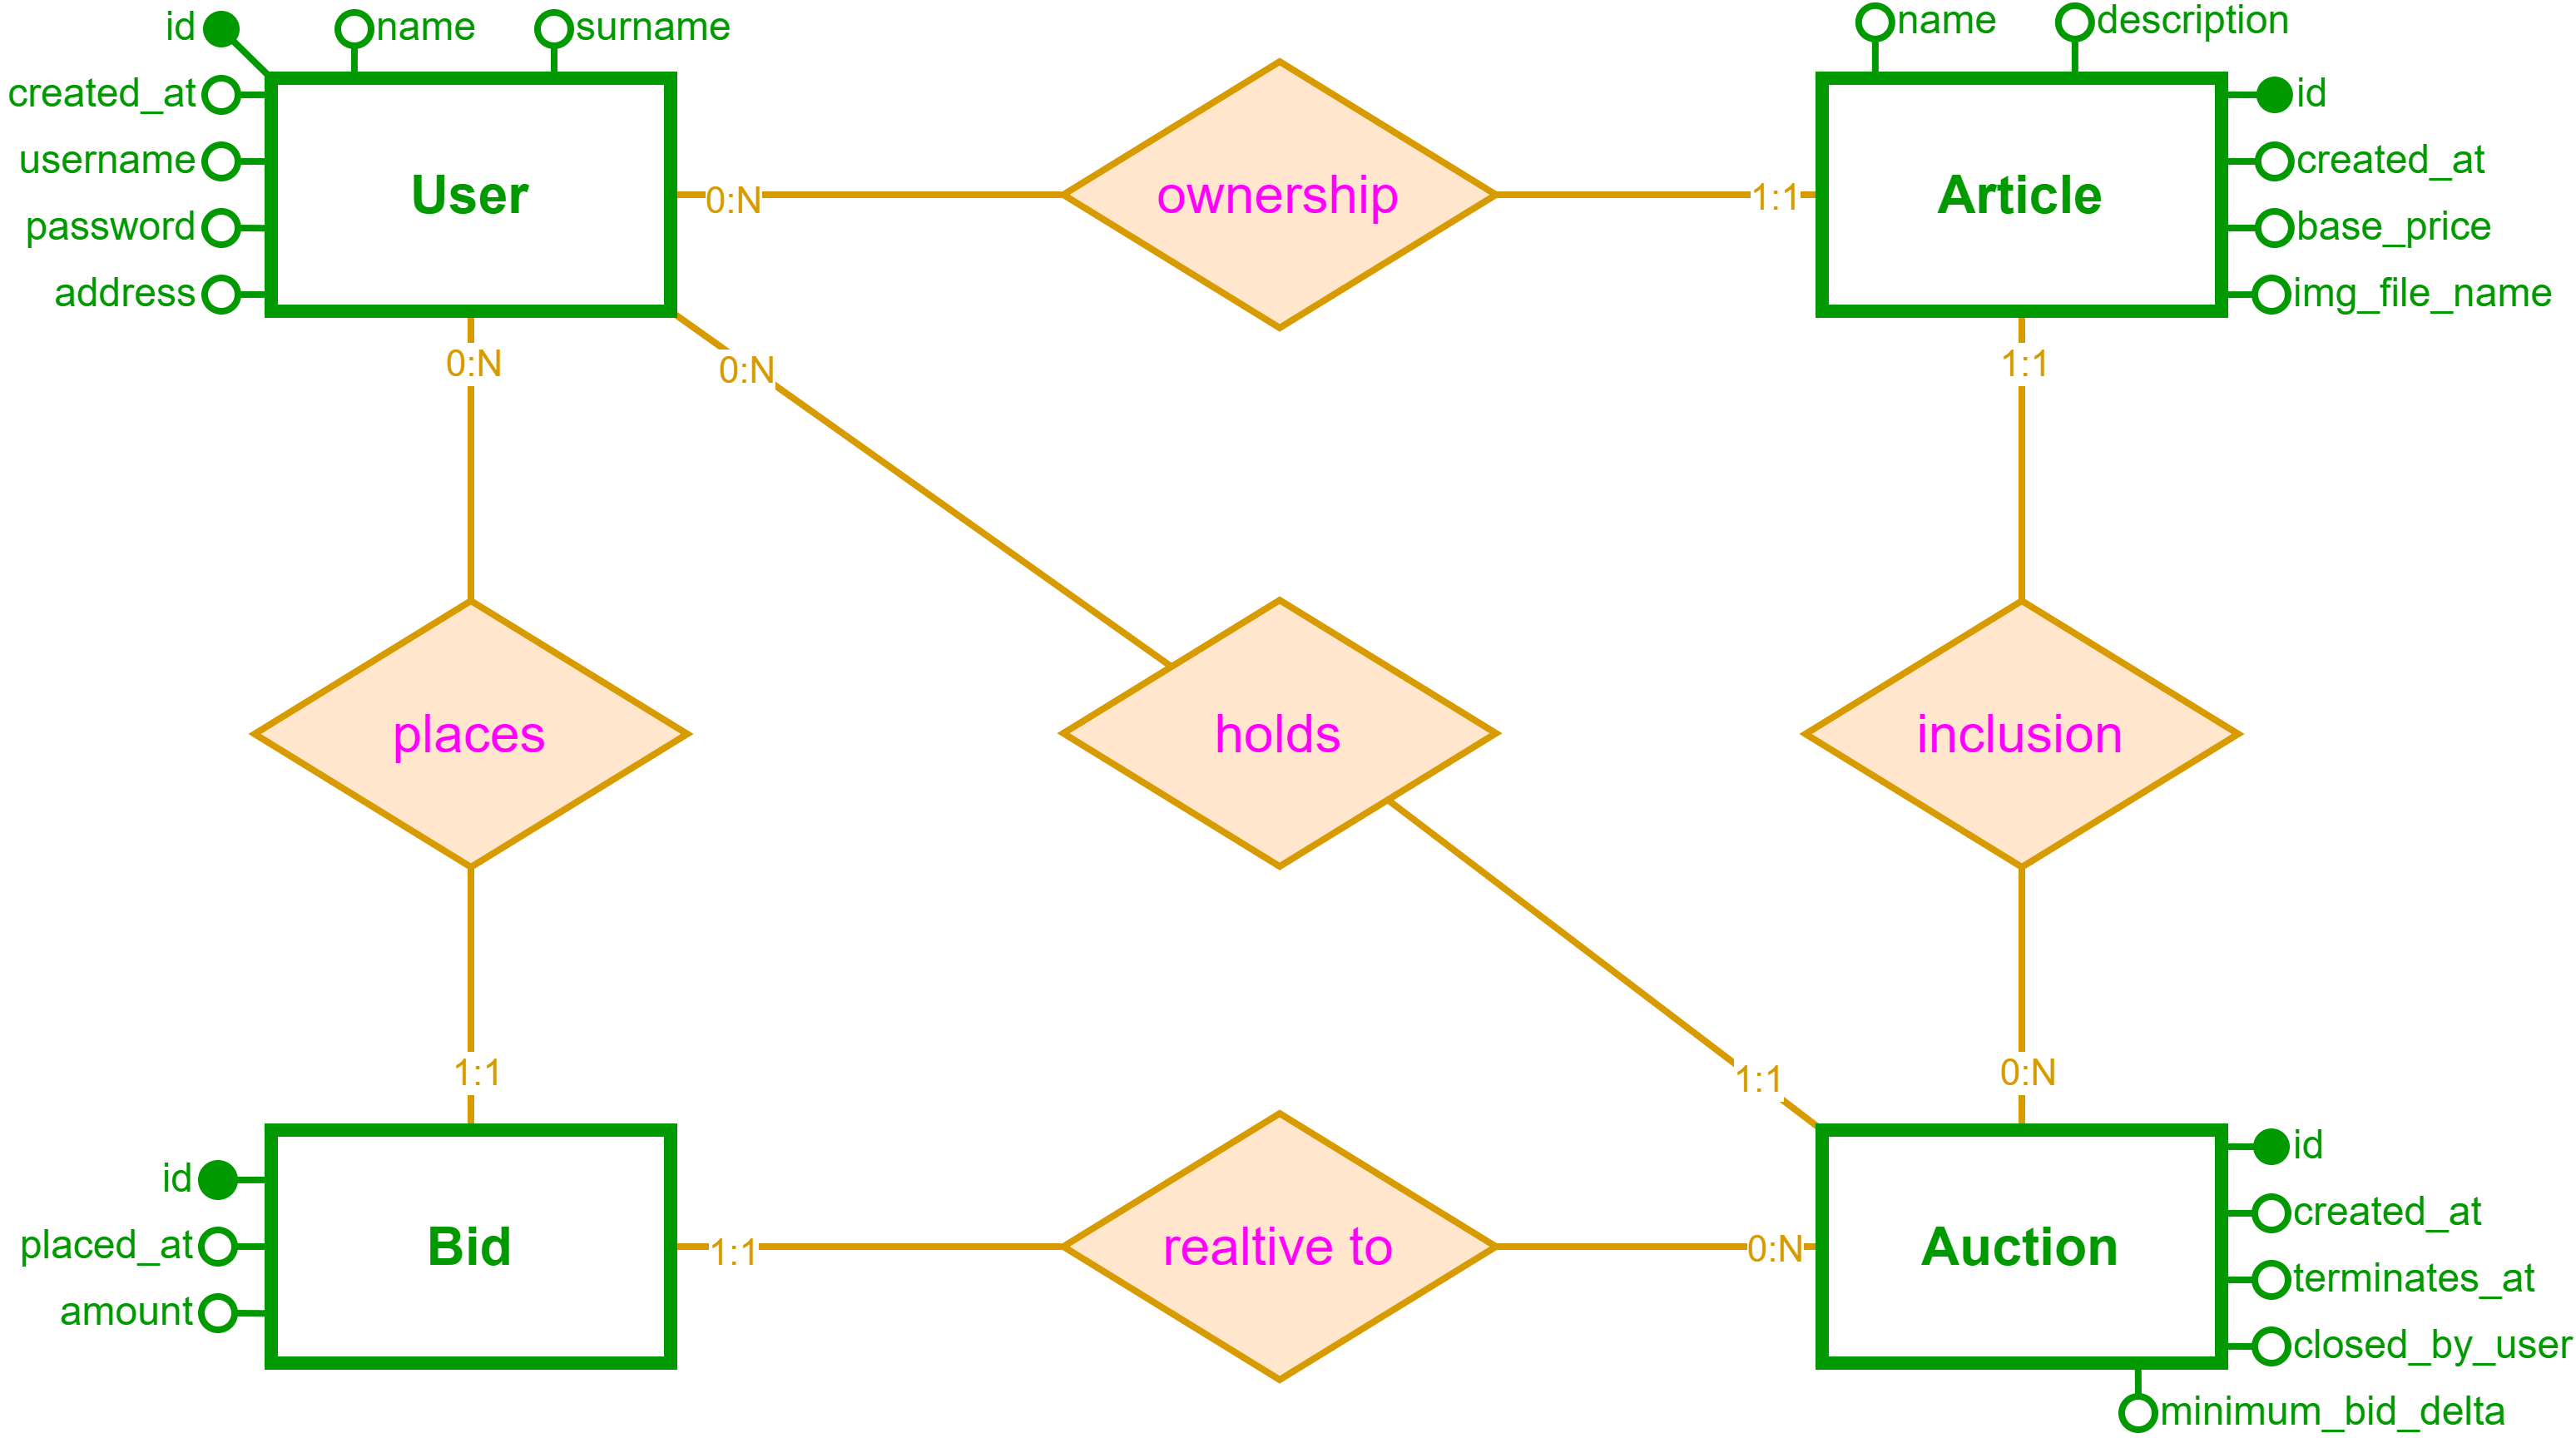
\includegraphics[width=1.2\textwidth]{TIW-ER.png}}
		\end{figure}
		\phantom{.}\\
		Attributes that store the timestamp of when a tuple is inserted, such as \textit{`created\_at`}, are not required for all entities. However, since their value can be automatically generated by the DB during the \textit{INSERT} phase at a negligible cost, it is preferable to include this information in the database as it might always be useful.

		\subsection{SQL Code for Tables}
		The following code, used to create the tables, shows the logical structure of the database.\\
		\subsubsection{User}
		\phantom{.}
		\begin{lstlisting}
			CREATE TABLE IF NOT EXISTS `users` (
			  `id` int(32) unsigned NOT NULL AUTO_INCREMENT,
			  `created_at` timestamp NOT NULL DEFAULT current_timestamp(),
			  `username` varchar(20) NOT NULL,
			  `password` varchar(40) NOT NULL,
			  `name` varchar(32) NOT NULL,
			  `surname` varchar(32) NOT NULL,
			  `address` varchar(50) NOT NULL,
			  PRIMARY KEY (`id`),
			  UNIQUE KEY `username` (`username`)
			);
		\end{lstlisting}
		\phantom{.}\\	

		\subsubsection{Article}
		\phantom{.}
		\begin{lstlisting}
			CREATE TABLE IF NOT EXISTS `articles` (
			  `id` int(32) unsigned NOT NULL AUTO_INCREMENT,
			  `owner_user_id` int(32) unsigned NOT NULL,
			  `created_at` timestamp NOT NULL DEFAULT current_timestamp(),
			  `base_price` decimal(20,2) NOT NULL,
			  `auction_id` int(32) unsigned DEFAULT NULL,
			  `name` varchar(32) NOT NULL,
			  `description` varchar(200) DEFAULT NULL,
			  `img_file_name` varchar(20) DEFAULT NULL,
			  PRIMARY KEY (`id`),
			  KEY `FK_articles_auctions` (`auction_id`),
			  KEY `FK_articles_users` (`owner_user_id`),
			  CONSTRAINT `FK_articles_auctions` FOREIGN KEY (`auction_id`) REFERENCES `auctions` (`id`) ON DELETE NO ACTION ON UPDATE CASCADE,
			  CONSTRAINT `FK_articles_users` FOREIGN KEY (`owner_user_id`) REFERENCES `users` (`id`) ON DELETE NO ACTION ON UPDATE CASCADE,
			  CONSTRAINT `positive_price` CHECK (`base_price` > 0)
			);
		\end{lstlisting}
		\phantom{.}\\

		\subsubsection{Bid}
		\phantom{.}
		\begin{lstlisting}
			CREATE TABLE IF NOT EXISTS `bids` (
			  `id` int(32) unsigned NOT NULL AUTO_INCREMENT,
			  `placed_at` timestamp NOT NULL DEFAULT current_timestamp(),
			  `bidder_user_id` int(32) unsigned NOT NULL,
			  `auction_id` int(32) unsigned NOT NULL,
			  `amount` decimal(20,2) unsigned NOT NULL,
			  PRIMARY KEY (`id`),
			  KEY `FK_bids_auctions` (`auction_id`),
			  KEY `FK_bids_users` (`bidder_user_id`),
			  CONSTRAINT `FK_bids_auctions` FOREIGN KEY (`auction_id`) REFERENCES `auctions` (`id`) ON DELETE NO ACTION ON UPDATE CASCADE,
			  CONSTRAINT `FK_bids_users` FOREIGN KEY (`bidder_user_id`) REFERENCES `users` (`id`) ON DELETE NO ACTION ON UPDATE CASCADE,
			  CONSTRAINT `positive_amount` CHECK (`amount` > 0)
			);
		\end{lstlisting}
		\phantom{.}\\
		
		\subsubsection{Auction}
		\phantom{.}
		\begin{lstlisting}
			CREATE TABLE IF NOT EXISTS `auctions` (
			  `id` int(32) unsigned NOT NULL AUTO_INCREMENT,
			  `creator_user_id` int(32) unsigned NOT NULL DEFAULT 0,
			  `created_at` timestamp NOT NULL DEFAULT current_timestamp(),
			  `terminates_at` timestamp NOT NULL,
			  `closed_by_user` bit(1) NOT NULL DEFAULT b'0',
			  `minimum_bid_wedge` int(32) unsigned NOT NULL,
			  PRIMARY KEY (`id`),
			  KEY `FK_auctions_users` (`creator_user_id`),
			  CONSTRAINT `FK_auctions_users` FOREIGN KEY (`creator_user_id`) REFERENCES `users` (`id`) ON DELETE NO ACTION ON UPDATE CASCADE,
			  CONSTRAINT `terminates_after_Created` CHECK (`terminates_at` > `created_at`),
			  CONSTRAINT `positive_bid_delta` CHECK (`minimum_bid_wedge` > 0)
			);
		\end{lstlisting}		
		

		\subsection{Trigger}
			In addition to the constraints on individual attributes and those imposed by the presence of \textit{foreign keys}, triggers are added (both \textit{AFTER INSERT} and \textit{AFTER UPDATE} on the appropriate tables) that execute a query and raise an SQL exception when non-conforming elements are found, causing the operation to fail. The following conditions are verified.\\
				\subsubsection{Article owner matches auction creator} For each item in an auction, the item\'s owner must match the auction\'s creator.
				\begin{lstlisting}
					DELIMITER //
					CREATE TRIGGER `new_article_belonging_to_auction_owner` AFTER INSERT ON `articles` FOR EACH ROW BEGIN
						IF EXISTS (
							SELECT * FROM auctions AS au
							JOIN articles AS ar
							ON ar.auction_id = au.id
							WHERE ar.owner_user_id != au.creator_user_id
							) THEN
								SIGNAL SQLSTATE '45000'
									SET MESSAGE_TEXT = 'New articles must belong to the auction owner';
						END IF;
					END//
					DELIMITER ;
				\end{lstlisting}
				\phantom{.}\\
				
				\subsubsection{Bid respects min bid delta} For each bid, the amount must be at least \textit{minimum\_bid\_delta} greater than the highest of the previous bids (where a bid is considered previous by using the \textit{placed\_at} field).
				\begin{lstlisting}
					DELIMITER //
					CREATE TRIGGER `new_bid_lower_than_delta` AFTER INSERT ON `bids` FOR EACH ROW BEGIN
						IF EXISTS (
							SELECT * FROM bids AS b1
							JOIN auctions AS a
							ON a.id = b1.auction_id
							WHERE b1.amount - a.minimum_bid_wedge < (
								SELECT max(amount) FROM bids AS b2
								WHERE b2.placed_at < b1.placed_at AND
									b2.auction_id = b1.auction_id )
							) THEN
								SIGNAL SQLSTATE '45000'
									SET MESSAGE_TEXT = 'New bids must respect minimum wedge';
						END IF;
					END//
					DELIMITER ;
				\end{lstlisting}
				\phantom{.}\\

				\subsubsection{No bids after termination} Bids cannot be placed if \textit{CURRENT\_TIMESTAMP()} is greater than the auction termination timestamp.
				\begin{lstlisting}
					DELIMITER //
					CREATE TRIGGER `new_bid_after_termination` AFTER INSERT ON `bids` FOR EACH ROW BEGIN
						IF EXISTS(
							SELECT * FROM auctions AS a
							WHERE a.id = NEW.auction_id AND
								a.terminates_at < CURRENT_TIMESTAMP()
						) THEN
							SIGNAL SQLSTATE '45000'
								SET MESSAGE_TEXT = 'New bids cannot be placed after auction termination';
						END IF;
					END//
					DELIMITER ;
				\end{lstlisting}
				\phantom{.}\\
				
				\subsubsection{Auction without articles} Every auction must have at least one article. This trigger must be temporarily disabled during the auction creation transaction, and the same \textit{AFTER UPDATE} check is present on the articles table. Since the DBMS in use does not allow disabling triggers, a variable is required.
				\begin{lstlisting}
					DELIMITER //
						CREATE TRIGGER `new_auction_without_articles` AFTER INSERT ON `auctions` FOR EACH ROW BEGIN
							IF (@AUCTION_TRIGGER_DISABLED IS NULL OR @AUCTION_TRIGGER_DISABLED!=1) AND EXISTS (
								SELECT id FROM auctions
								EXCEPT
								SELECT au.id FROM auctions AS au
								JOIN articles AS ar
								ON au.id = ar.auction_id
							) THEN
								SIGNAL SQLSTATE '45000'
									SET MESSAGE_TEXT = 'Each auction must have at least one article';
						END IF;
					END//
					DELIMITER ;
				\end{lstlisting}
		\section[PureHTML - Application Design]{Application Design for the Pure HTML Version}
			\subsection{Servlet Structure}
			\phantom{.}\\
				\noindent \makebox[\textwidth]{
				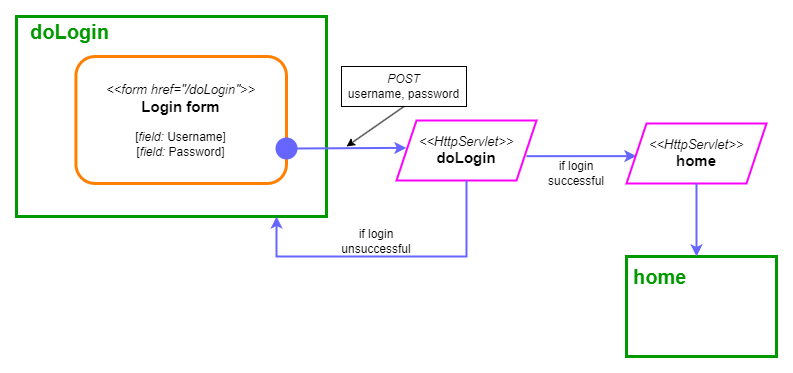
\includegraphics[width=1.1\textwidth]{Servlets/TIW-doLogin.png}}
			\phantom{.}
				\noindent \makebox[\textwidth]{
				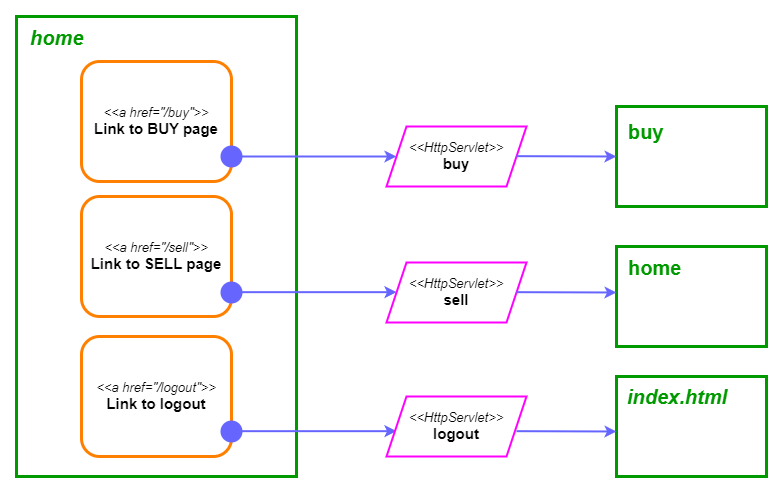
\includegraphics[width=1.1\textwidth]{Servlets/TIW-home.png}}
			\newpage
			\phantom{.}
				\noindent \makebox[\textwidth]{
				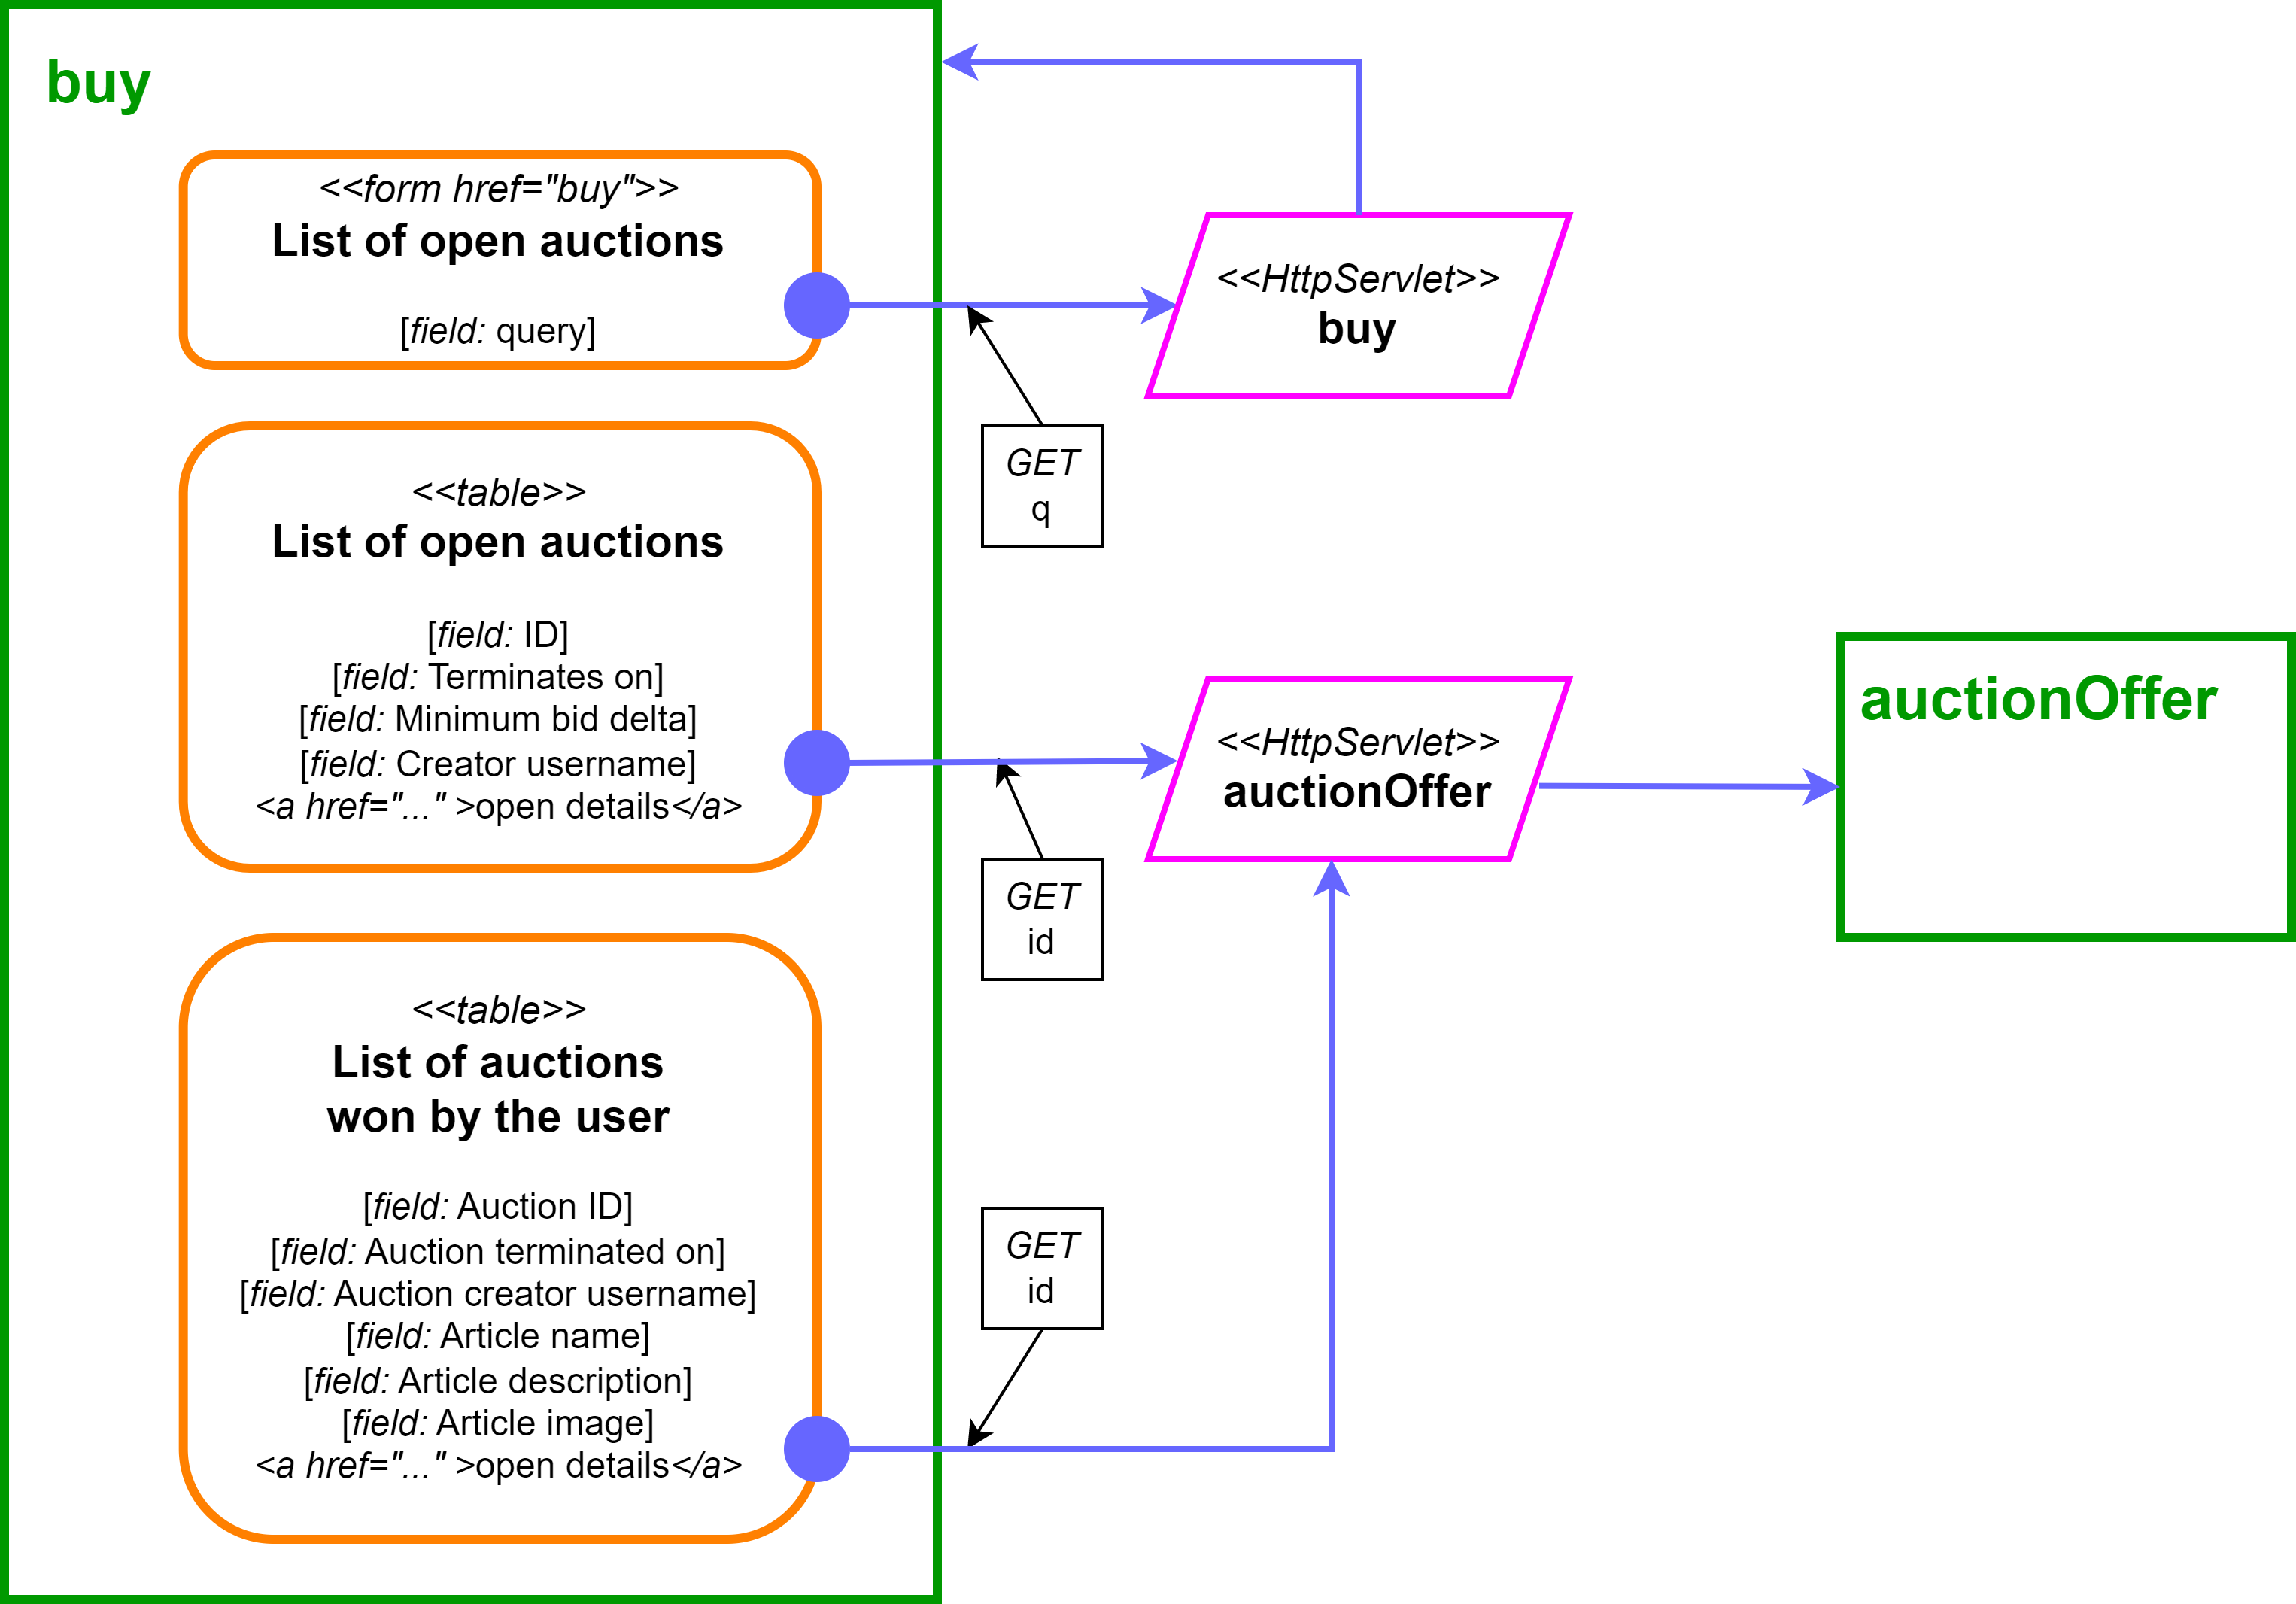
\includegraphics[width=1\textwidth]{Servlets/TIW-buy.png}}
			\phantom{.}
				\noindent \makebox[\textwidth]{
				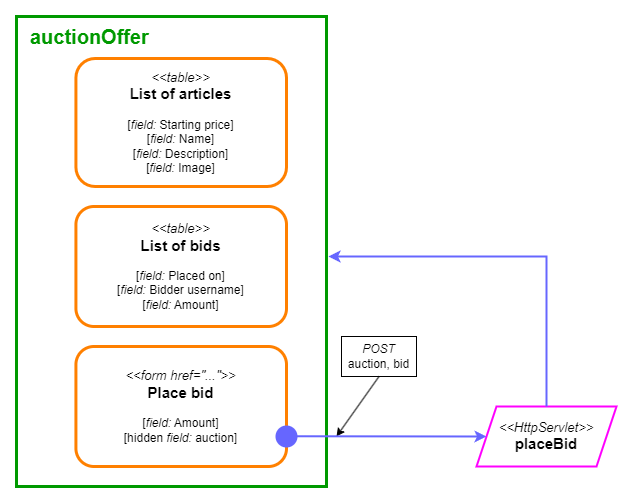
\includegraphics[width=1\textwidth]{Servlets/TIW-auctionOffer.png}}
			\newpage
			\phantom{.}
				\noindent \makebox[\textwidth]{
				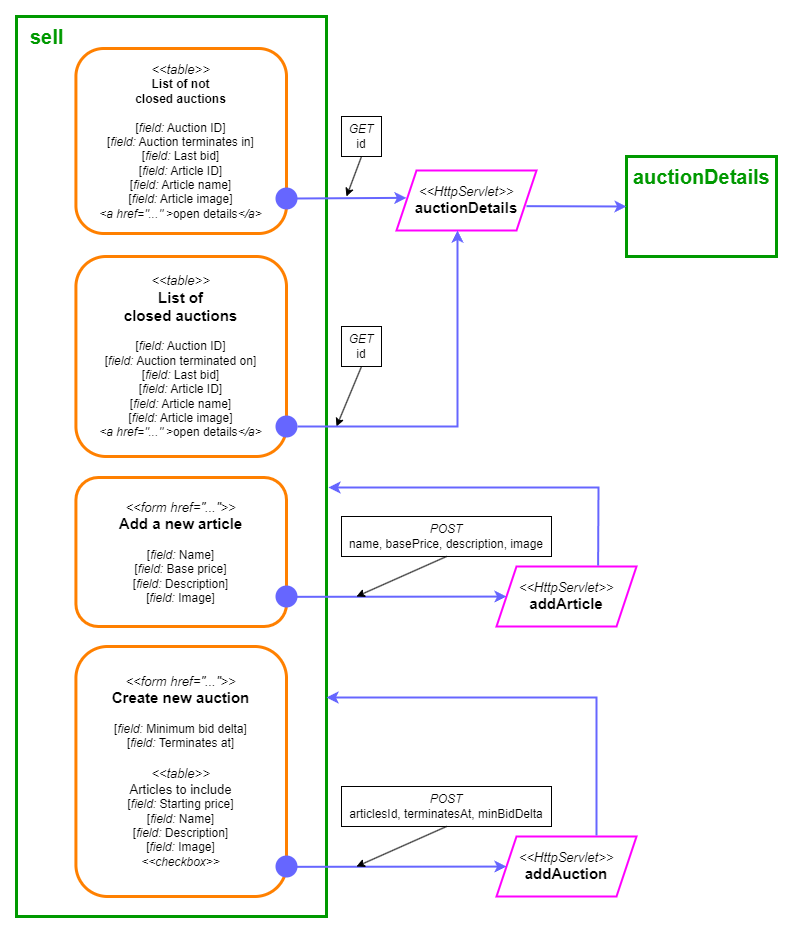
\includegraphics[width=0.95\textwidth]{Servlets/TIW-sell.png}}
			\phantom{.}
				\noindent \makebox[\textwidth]{
				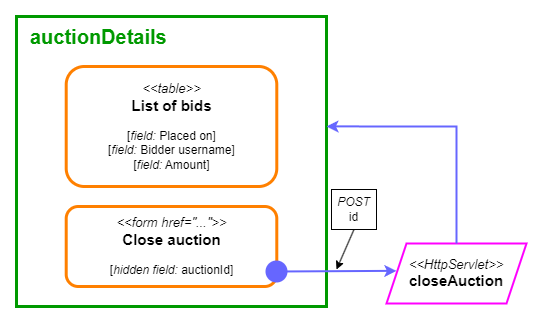
\includegraphics[width=0.65\textwidth]{Servlets/TIW-auctionDetails.png}}
			\phantom{.}
			\newpage
		\subsection{Navigation Elements}
			To improve the usability of the application, a navigation menu is added to all pages, allowing users to reach the home, buy, and sell pages, and to log out. This element is positioned on the side using appropriate CSS definitions, and to include the HTML text, the \textit{th:insert} functionality of Thymeleaf is used. This way, the same HTML code for displaying common elements is automatically inserted on all pages.
			\begin{figure}[h]
				\noindent \makebox[\textwidth]{
				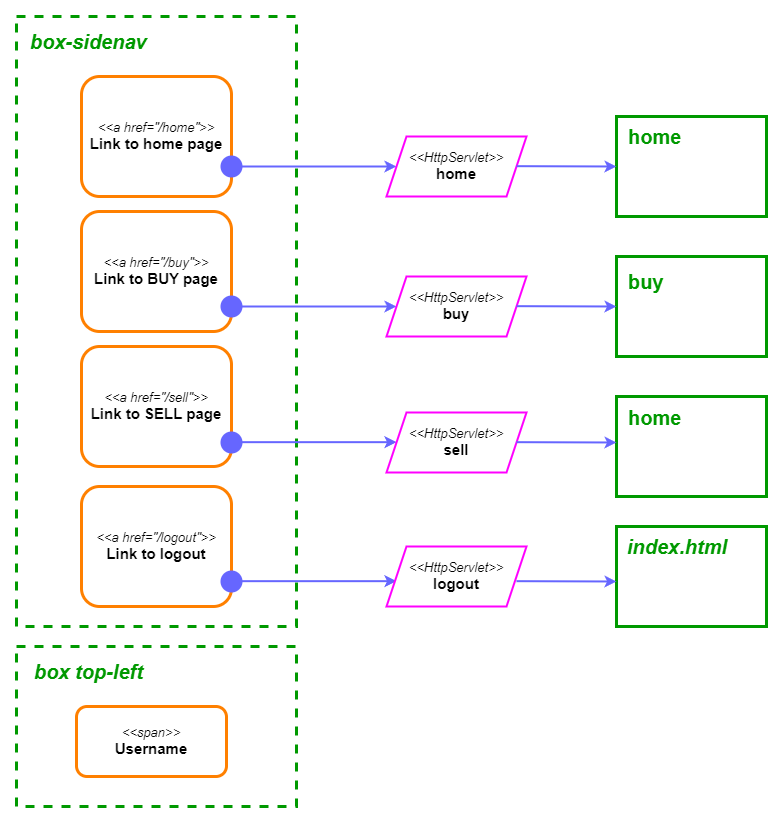
\includegraphics[width=1\textwidth]{Servlets/TIW-fragment.png}}
			\end{figure}
			\phantom{.}
		\subsection{Access Control}
			All servlets (except for doLogin and logout) require that the \textit{user} attribute in the session contains an object of type User. This requirement is both practical (the data of that object are needed) and functional (only authenticated users can use the application). To ensure this, a loginChecker servlet of type \textit{Filter} is used. This implements a function that redirects the user to the login page if they are not authenticated.
		\section[PureHTML - Components]{Components for the Pure HTML Version}
			\subsection{Database Access}\label{accessodb}
			To manage database connections, a class called ConnectionHandler has been implemented, with servlets using the \textit{getConnection} and \textit{returnConnection} methods. This class ensures that:
			\begin{itemize}
				\item there is no excessive number of open connections to the database,
				\item no connection stays open for too long without being used,
				\item servlets (when possible) obtain a connection from those that are ready (not yet closed) rather than creating a new one.
			\end{itemize}
			To achieve this, a consumer-producer pattern typical of multithreading programming is used, along with an asynchronous \textit{Runnable} that manages the list of open connections.
			By using this utility class, the servlets do not need to open database connections during initialization and store them. For this reason, the functionality of DAO objects has been implemented through static methods in the Bean classes.
			\subsection{Data Beans}\label{databeans}
			\begin{itemize}
				\item \textbf{User}
				\item \textbf{Article}
				\item \textbf{Bid}
				\item \textbf{Auction}, with the addition of the subclasses \textbf{AuctionClosed} and \textbf{AuctionWithArticles}
			\end{itemize}
			\subsection{DAO Functionality}\label{dao}
			To ensure greater robustness and facilitate debugging of the following functions, automatic tests have been implemented using the junit framework integrated with maven. This allows the correctness of the interaction with the database to be verified during the compilation phase. Although the work done is far from a "test-driven development" paradigm, also due to the stateful nature of the operations being tested, the simple tests performed ensure the correct functioning of a portion of the code.
			\subsubsection{User}
			\begin{itemize}
				\item loadWithCreds(username, password)
				\item loadWithId(id)
				\item loadWithUsername(username)
			\end{itemize}
			\phantom{.}\\
			\subsubsection{Article}
			\begin{itemize}
				\item getArticlesByAuction(auction\_id)
				\item getArticlesByUser(user\_id)
				\item createArticle(owner\_user\_id, base\_price, name, description, imagePart)
				\item checkOwner(user\_id, articles\_id)
			\end{itemize}
			\phantom{.}\\
			\subsubsection{Bid}
			\begin{itemize}
				\item getBidsPerAuction(auction\_id)
				\item getBidsPerUser(user)
				\item placeBid(bidder\_user\_id, auction\_id, amount)
			\end{itemize}
			\phantom{.}\\
			\subsubsection{Auction}
			\begin{itemize}
				\item getAuctionFromId(id)
				\item getAuctions()
				\item getAuctionsPerUser(user\_id)
				\item getAuctionsWonByUser(user\_id)
				\item getAuctionsWithSearch(expression)
				\item getMultipleAuctionWithArticles(auctionList)
				\item closeAuction(auction\_id)
				\item createAuction(creator\_user\_id, terminates\_at, minimum\_bid\_delta, articles\_id)
			\end{itemize}
		\subsection{Servlets}
			\subsubsection{Controllers}
				\begin{itemize}
					\item doLogin
					\item home
					\item buy
					\item auctionOffer
					\item placeBid
					\item sell
					\item auctionDetails
					\item addArticle
					\item addAuction
					\item closeAuction
					\item logout
				\end{itemize}
				\phantom{.}\\
			\subsubsection{Filters}
				\begin{itemize}
					\item loginChecker
				\end{itemize}
				\phantom{.}\\
			\subsection{Thymeleaf Template}
				\begin{itemize}
					\item index
					\item home
					\item buy
					\item auctionOffer
					\item sell
					\item auctionDetails
					\item header, this is a fragment
				\end{itemize}
		\section[PureHTML - Events and Sequence Diagrams]{Events and Sequence Diagrams for the Pure HTML Version}
			\subsubsection{A user logs in}
			\phantom{.}\\
			\noindent \makebox[\textwidth]{
				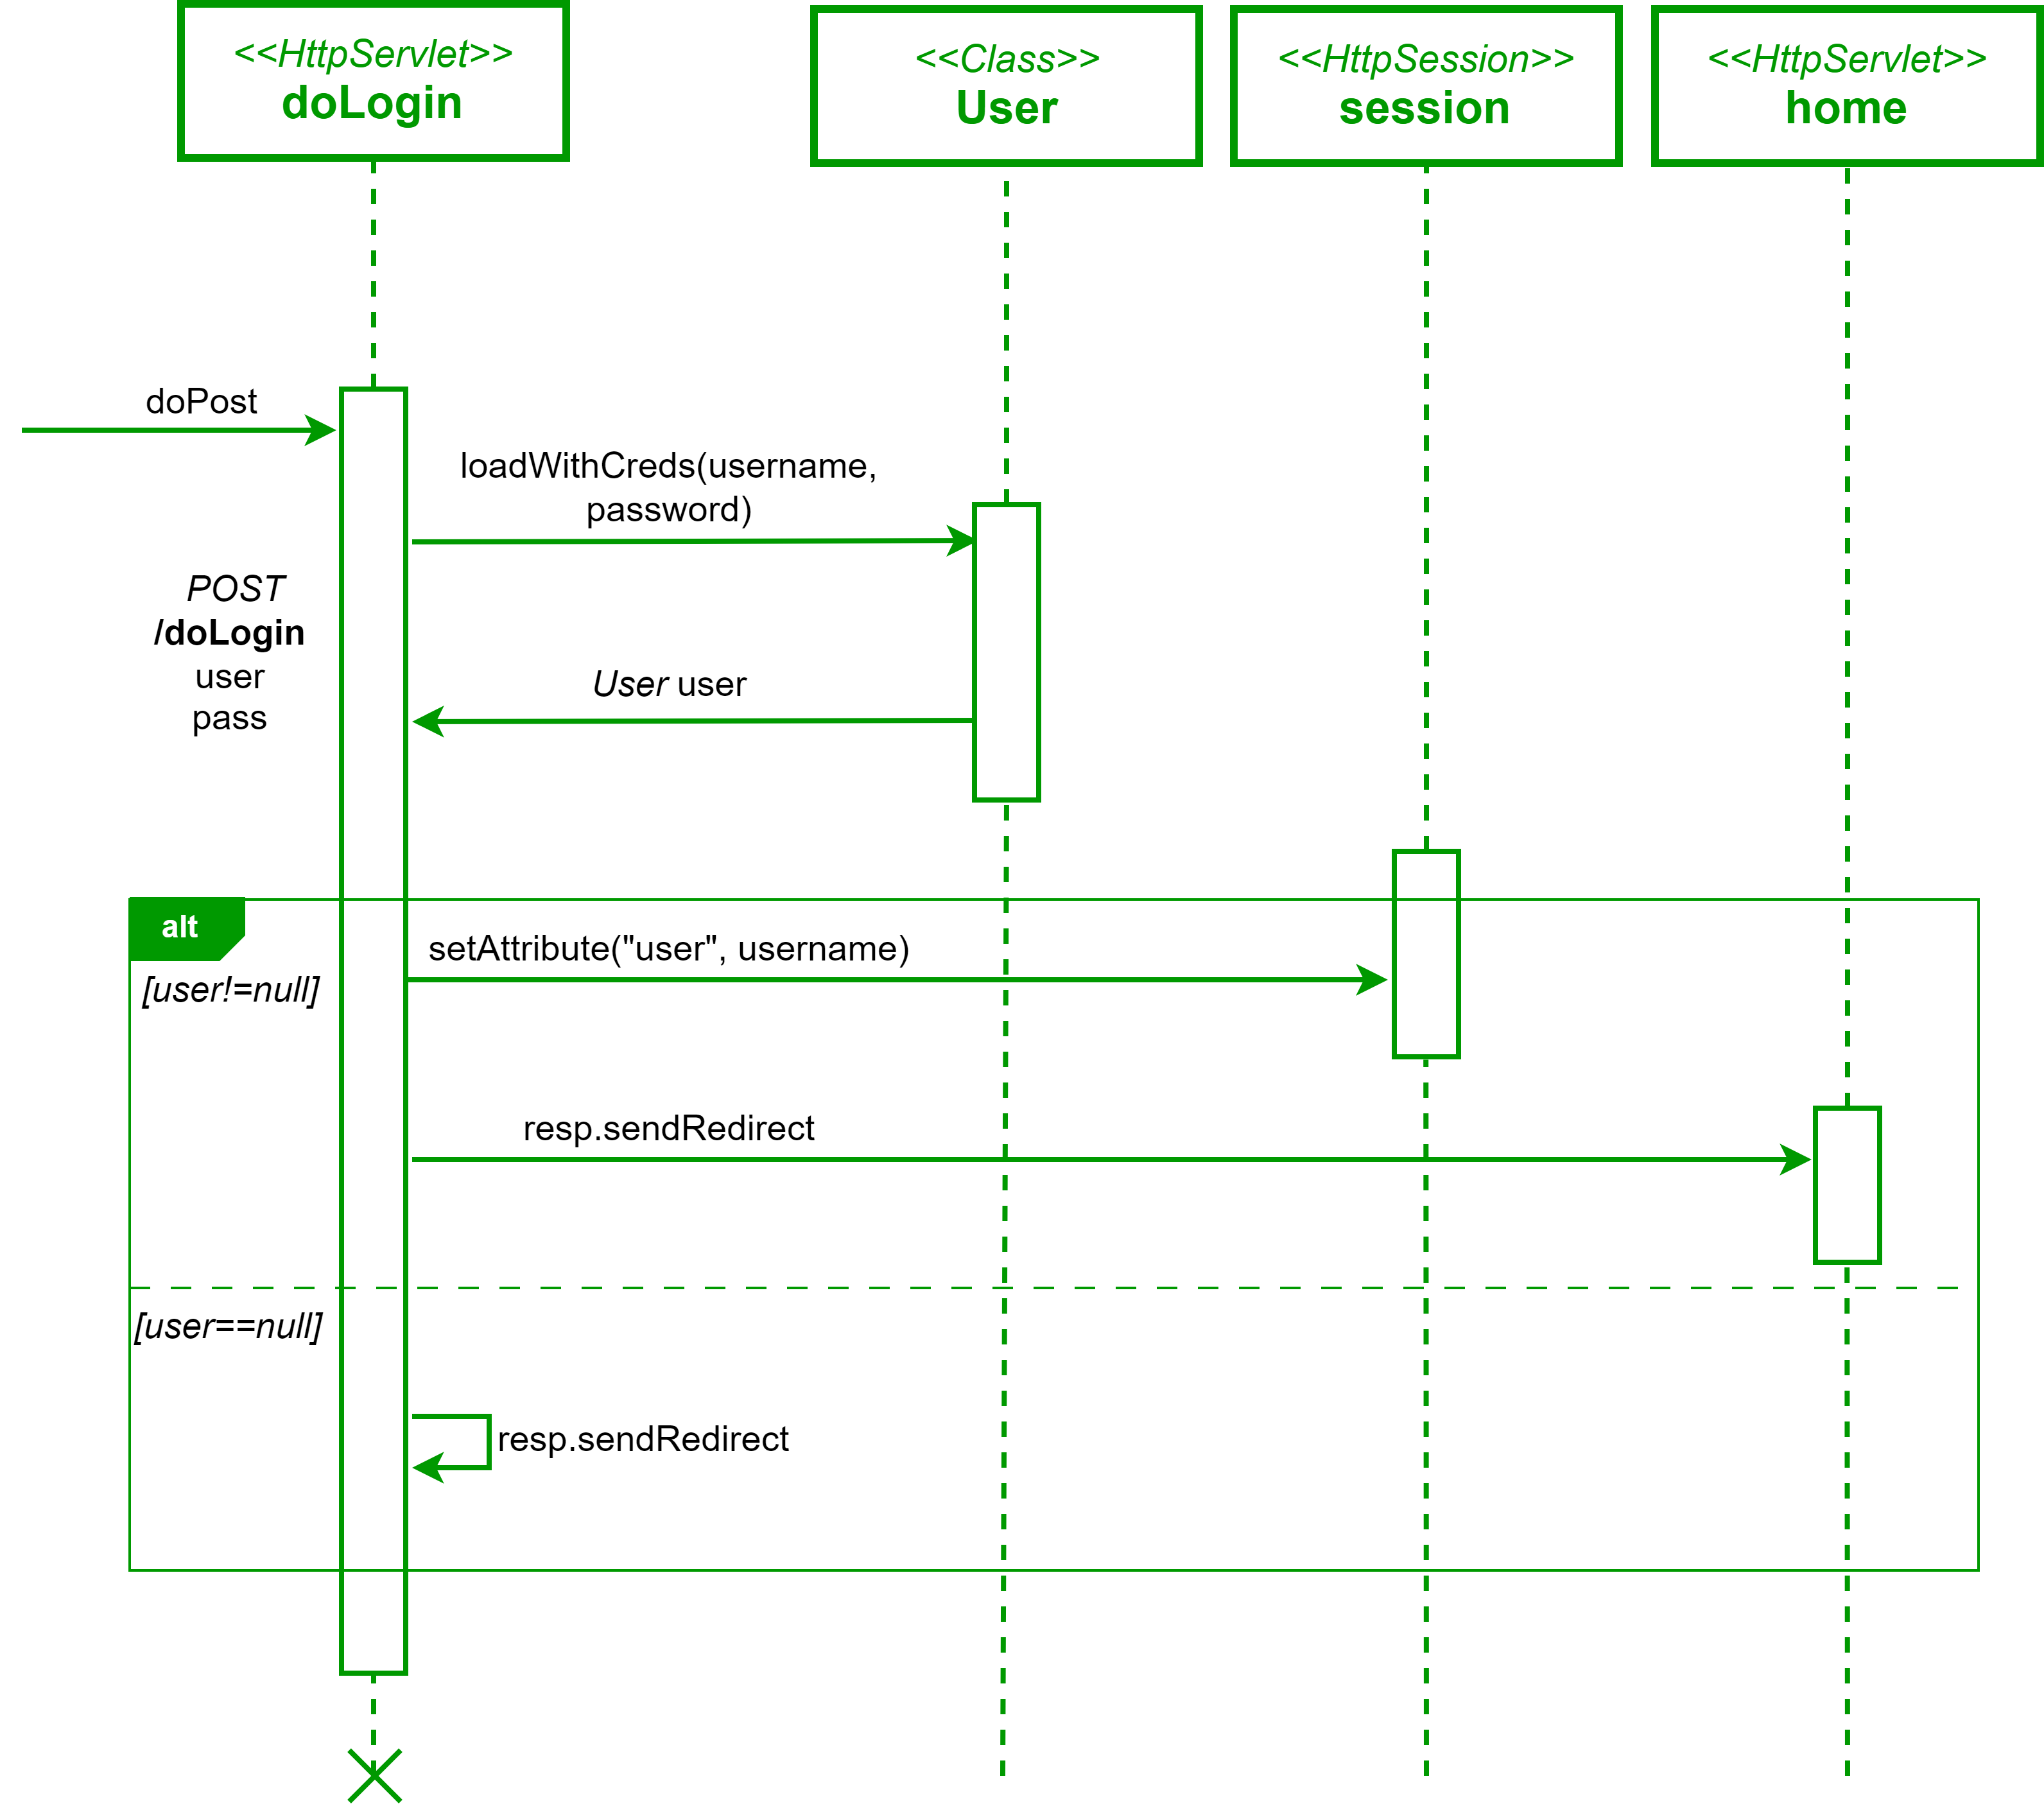
\includegraphics[width=1.2\textwidth]{SequenceDiagrams/TIW-login.png}}
			\phantom{.}\\
			\newpage
			
			\subsubsection{A user requests the BUY page}
			\phantom{.}\\
			\noindent \makebox[\textwidth]{
				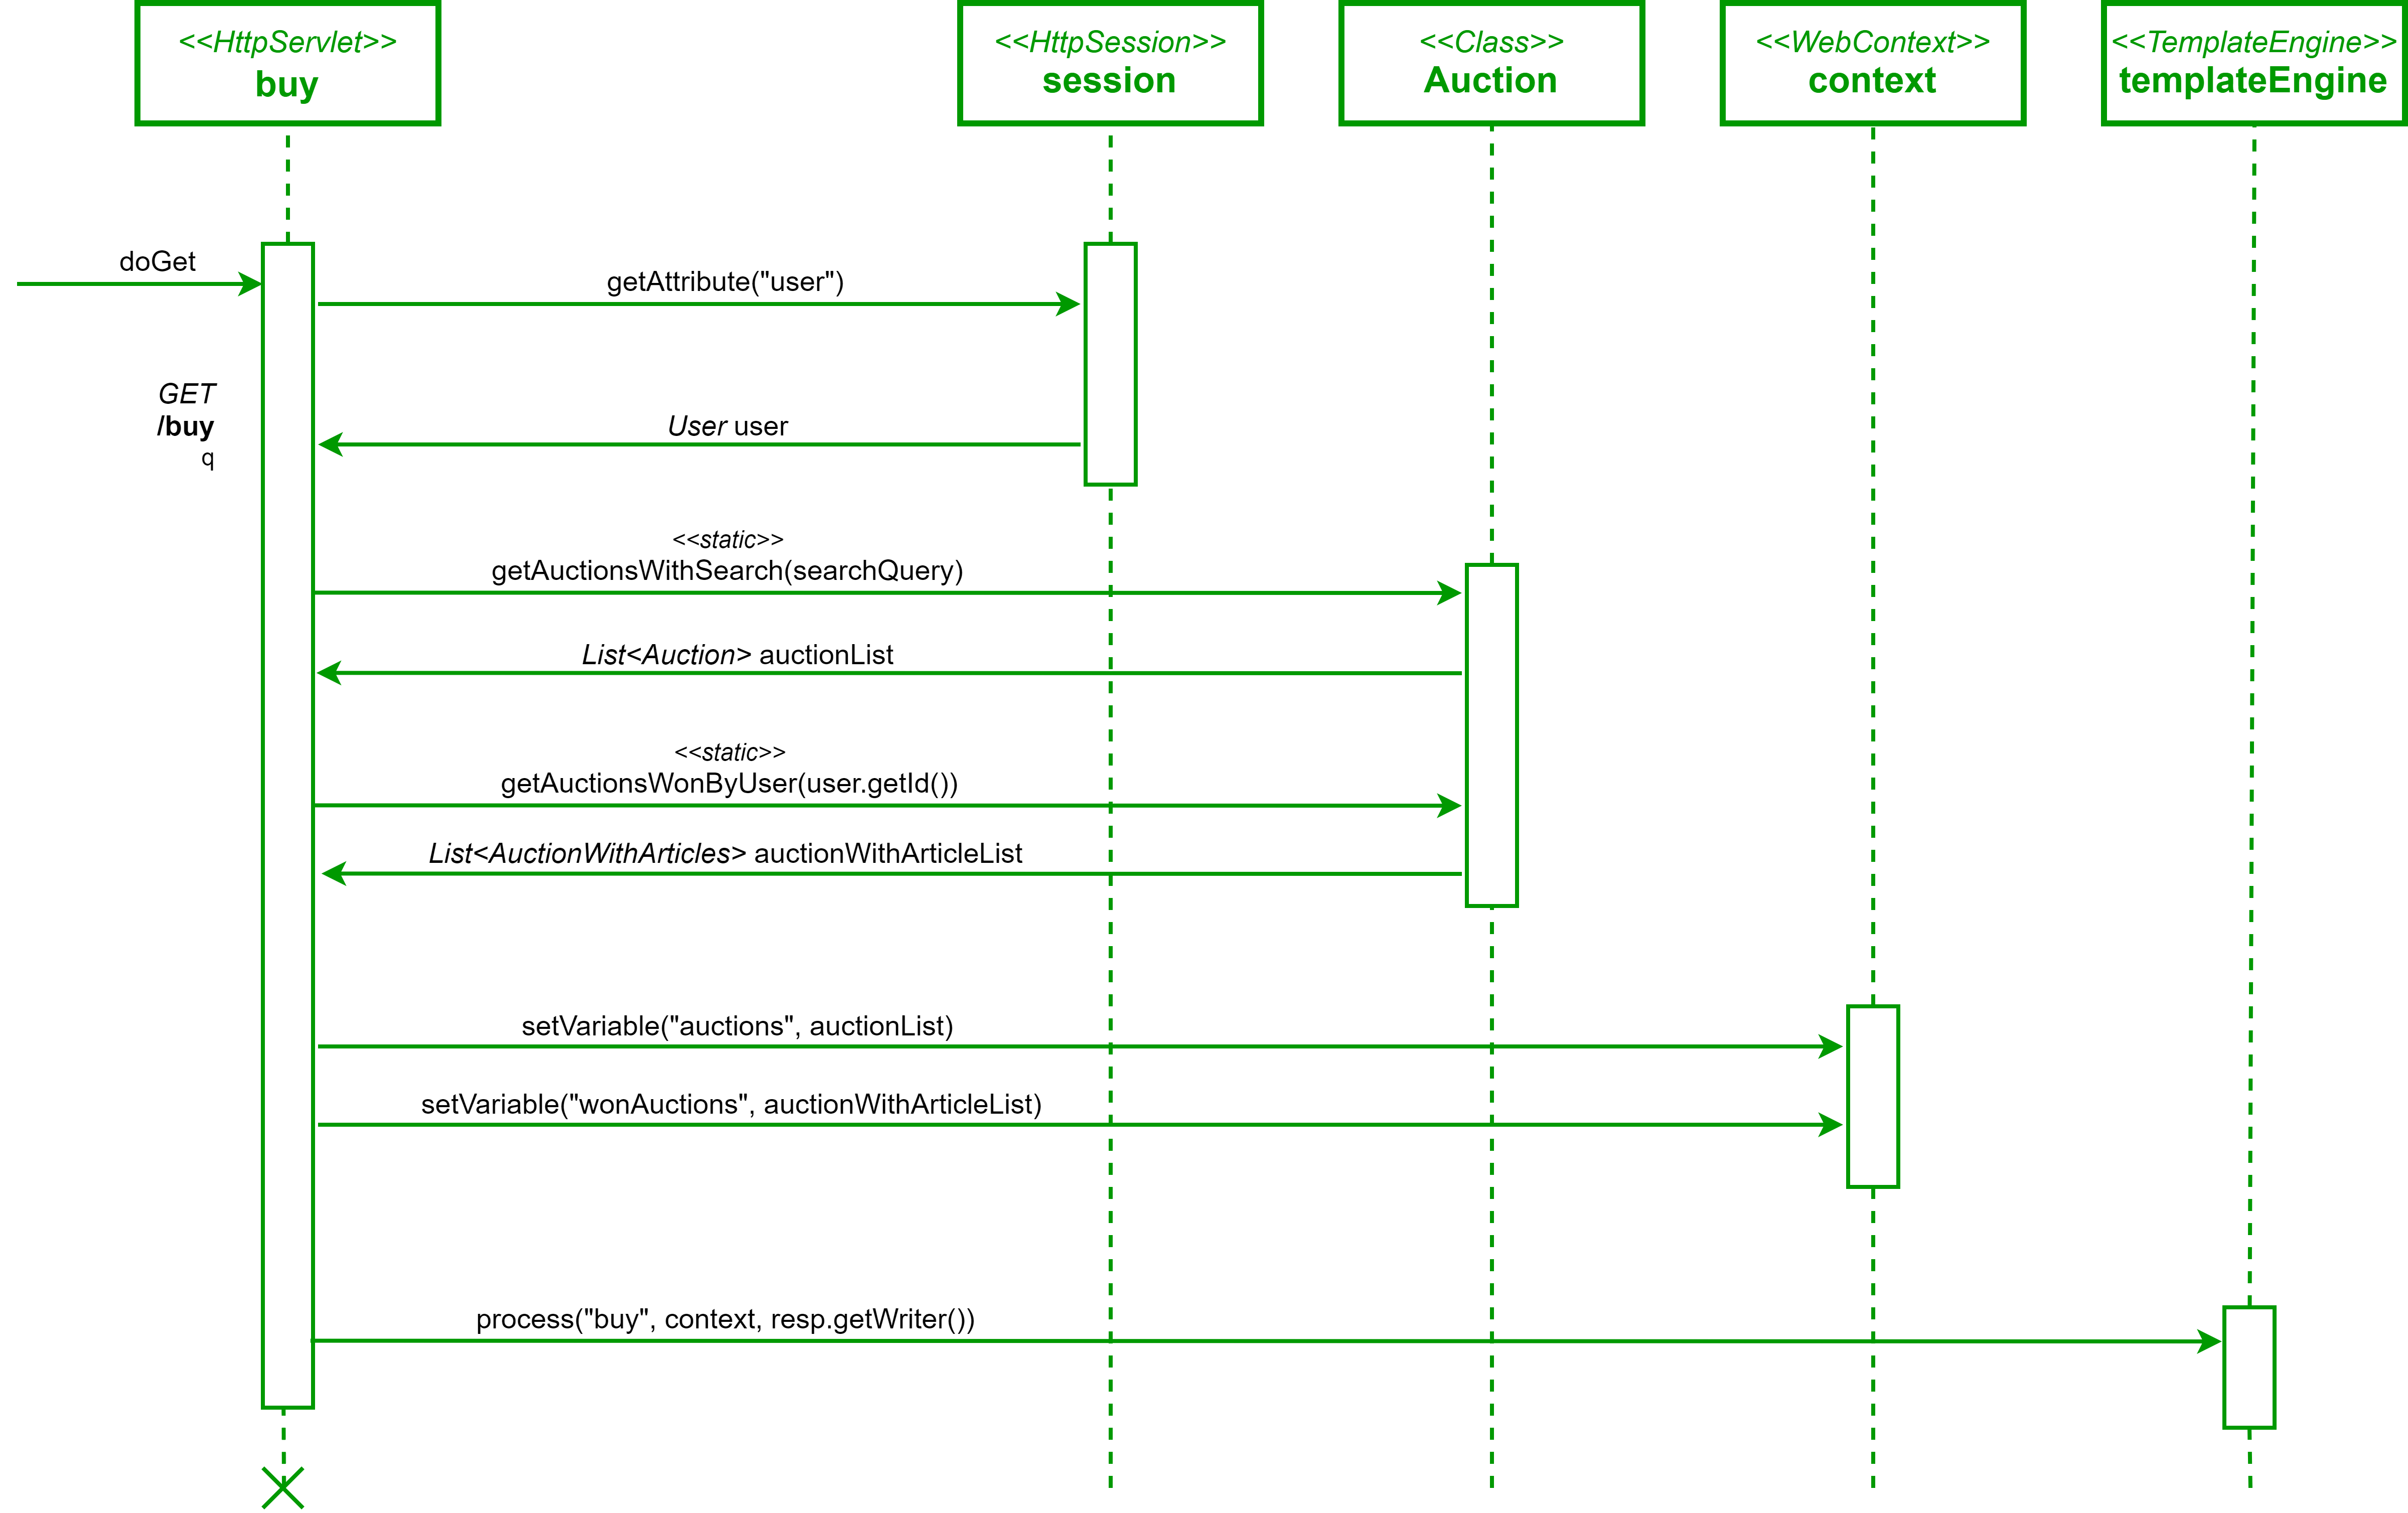
\includegraphics[width=1.1\textwidth]{SequenceDiagrams/TIW-buy.png}}
			\phantom{.}\\
			\subsubsection{A user requests the details page of an auction}
			\phantom{.}\\
			\noindent \makebox[\textwidth]{
				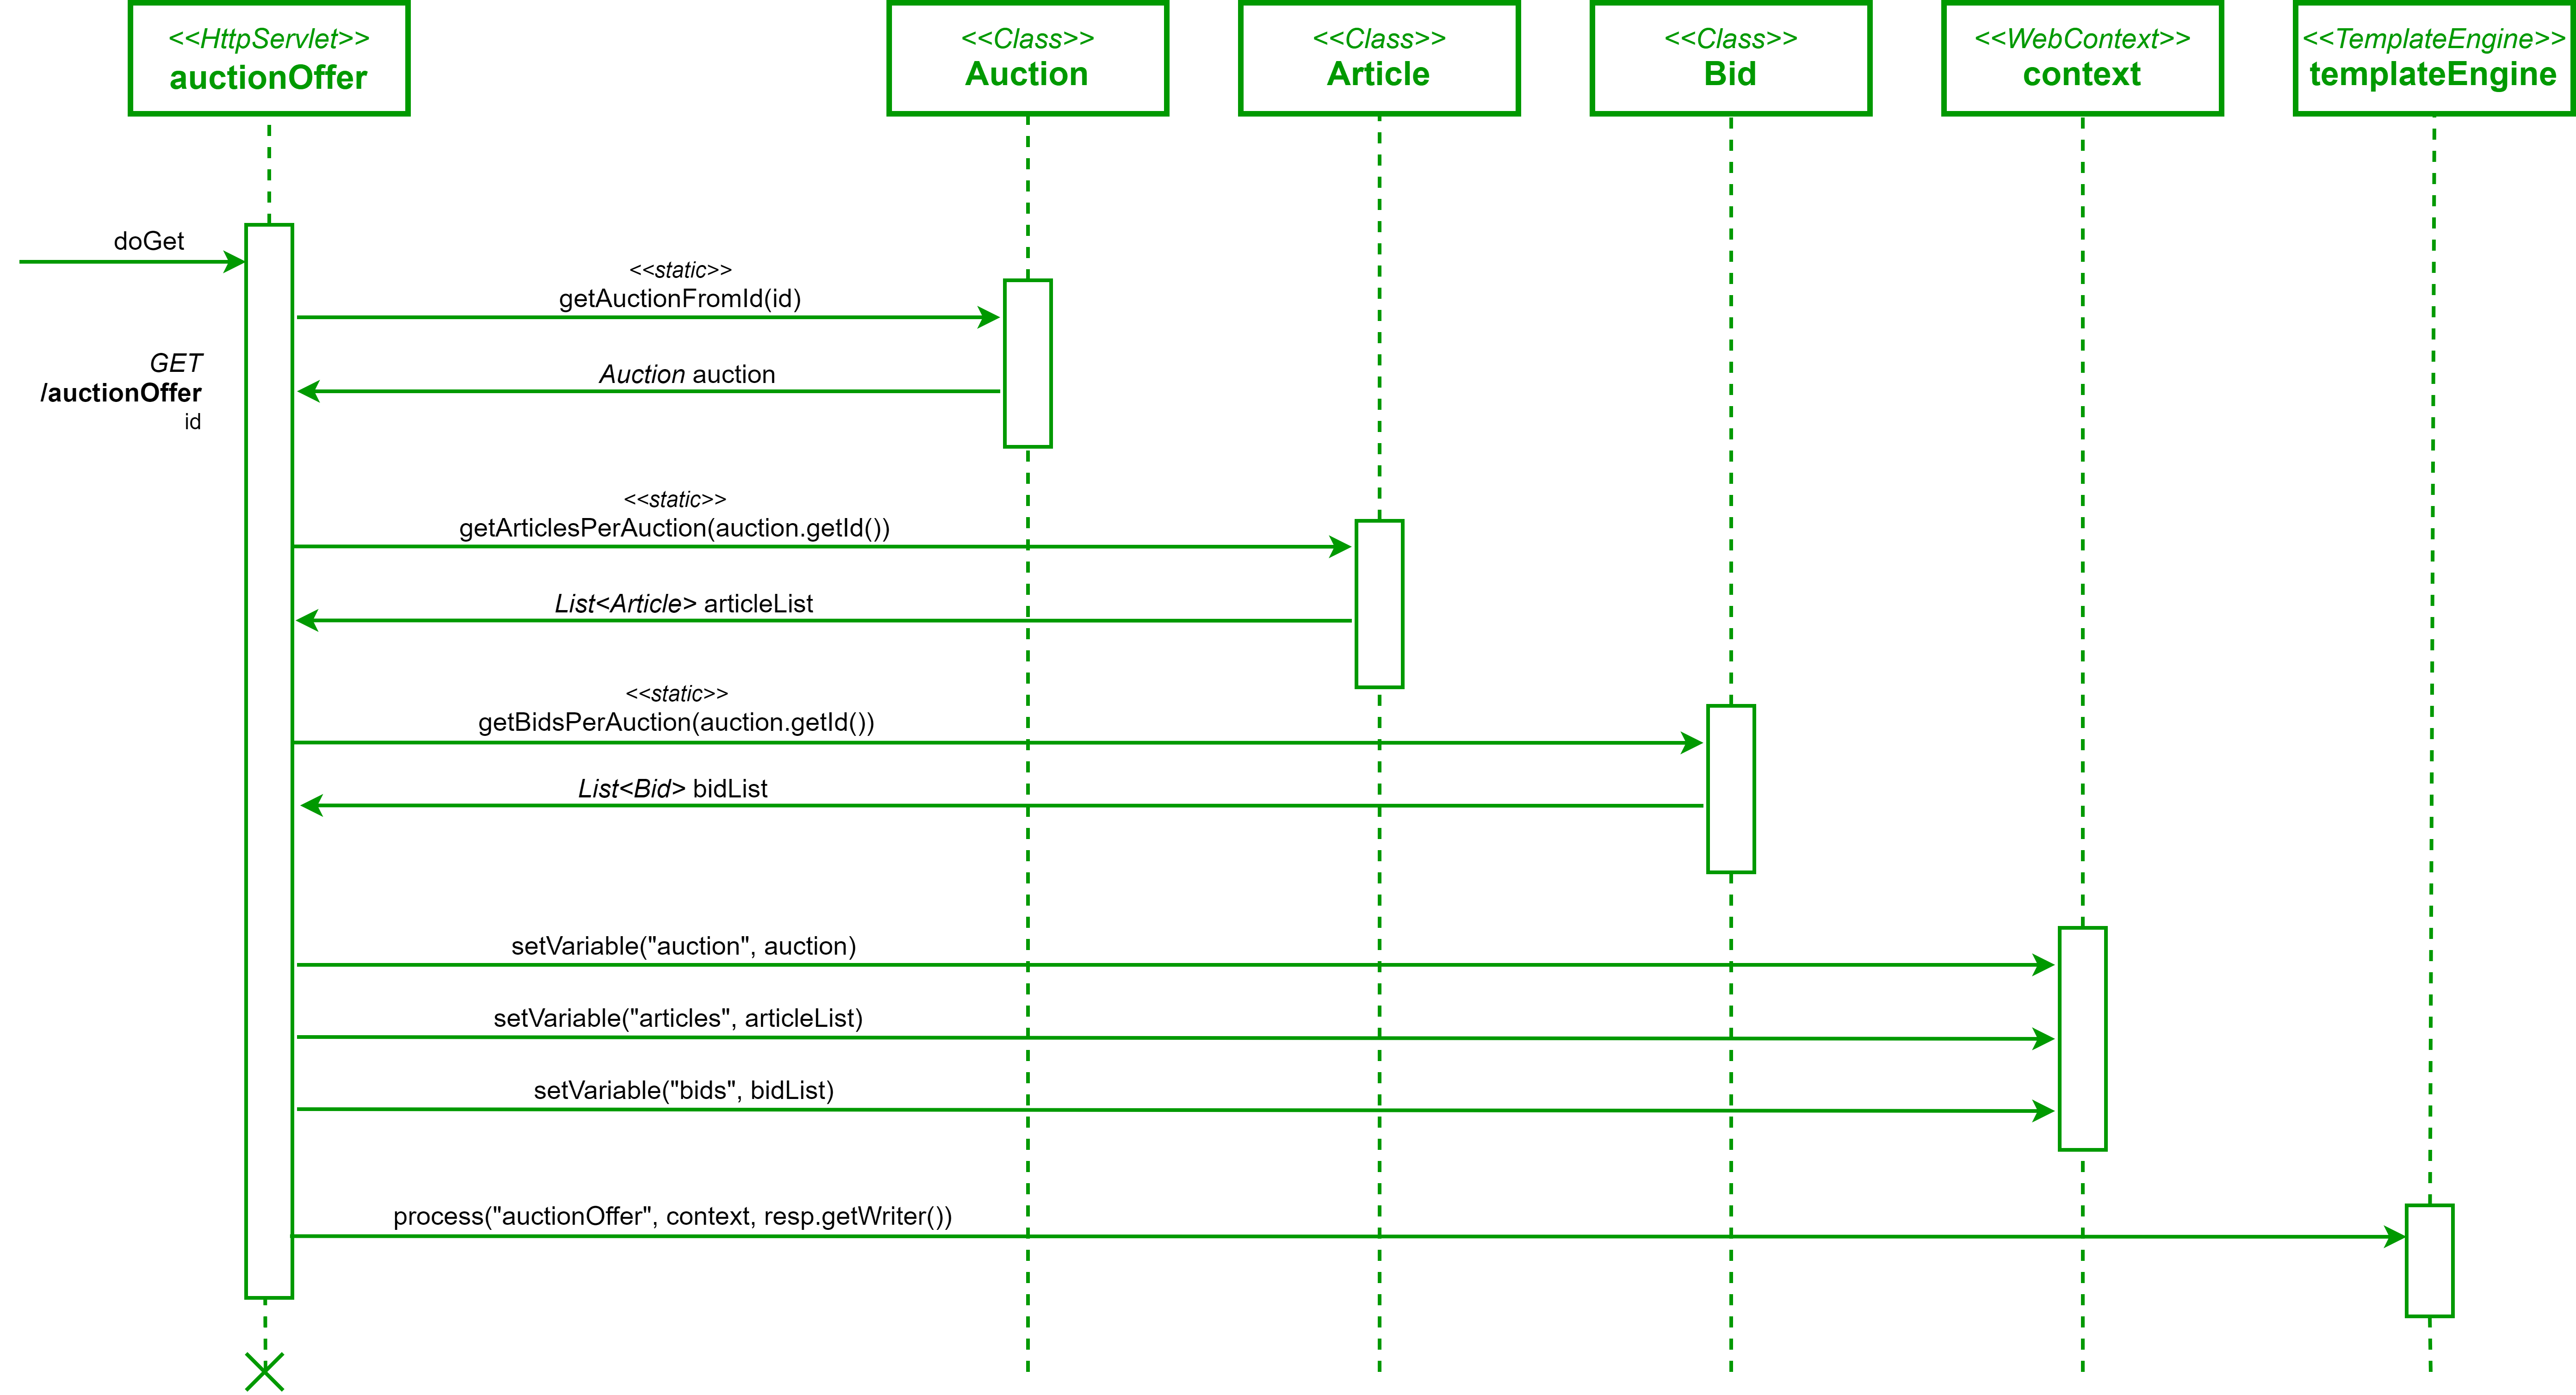
\includegraphics[width=1.12\textwidth]{SequenceDiagrams/TIW-auctionOffer.png}}	
			\phantom{.}\\
			\newpage
			\subsubsection{A user places a new bid}
			\phantom{.}\\
			\noindent \makebox[\textwidth]{
				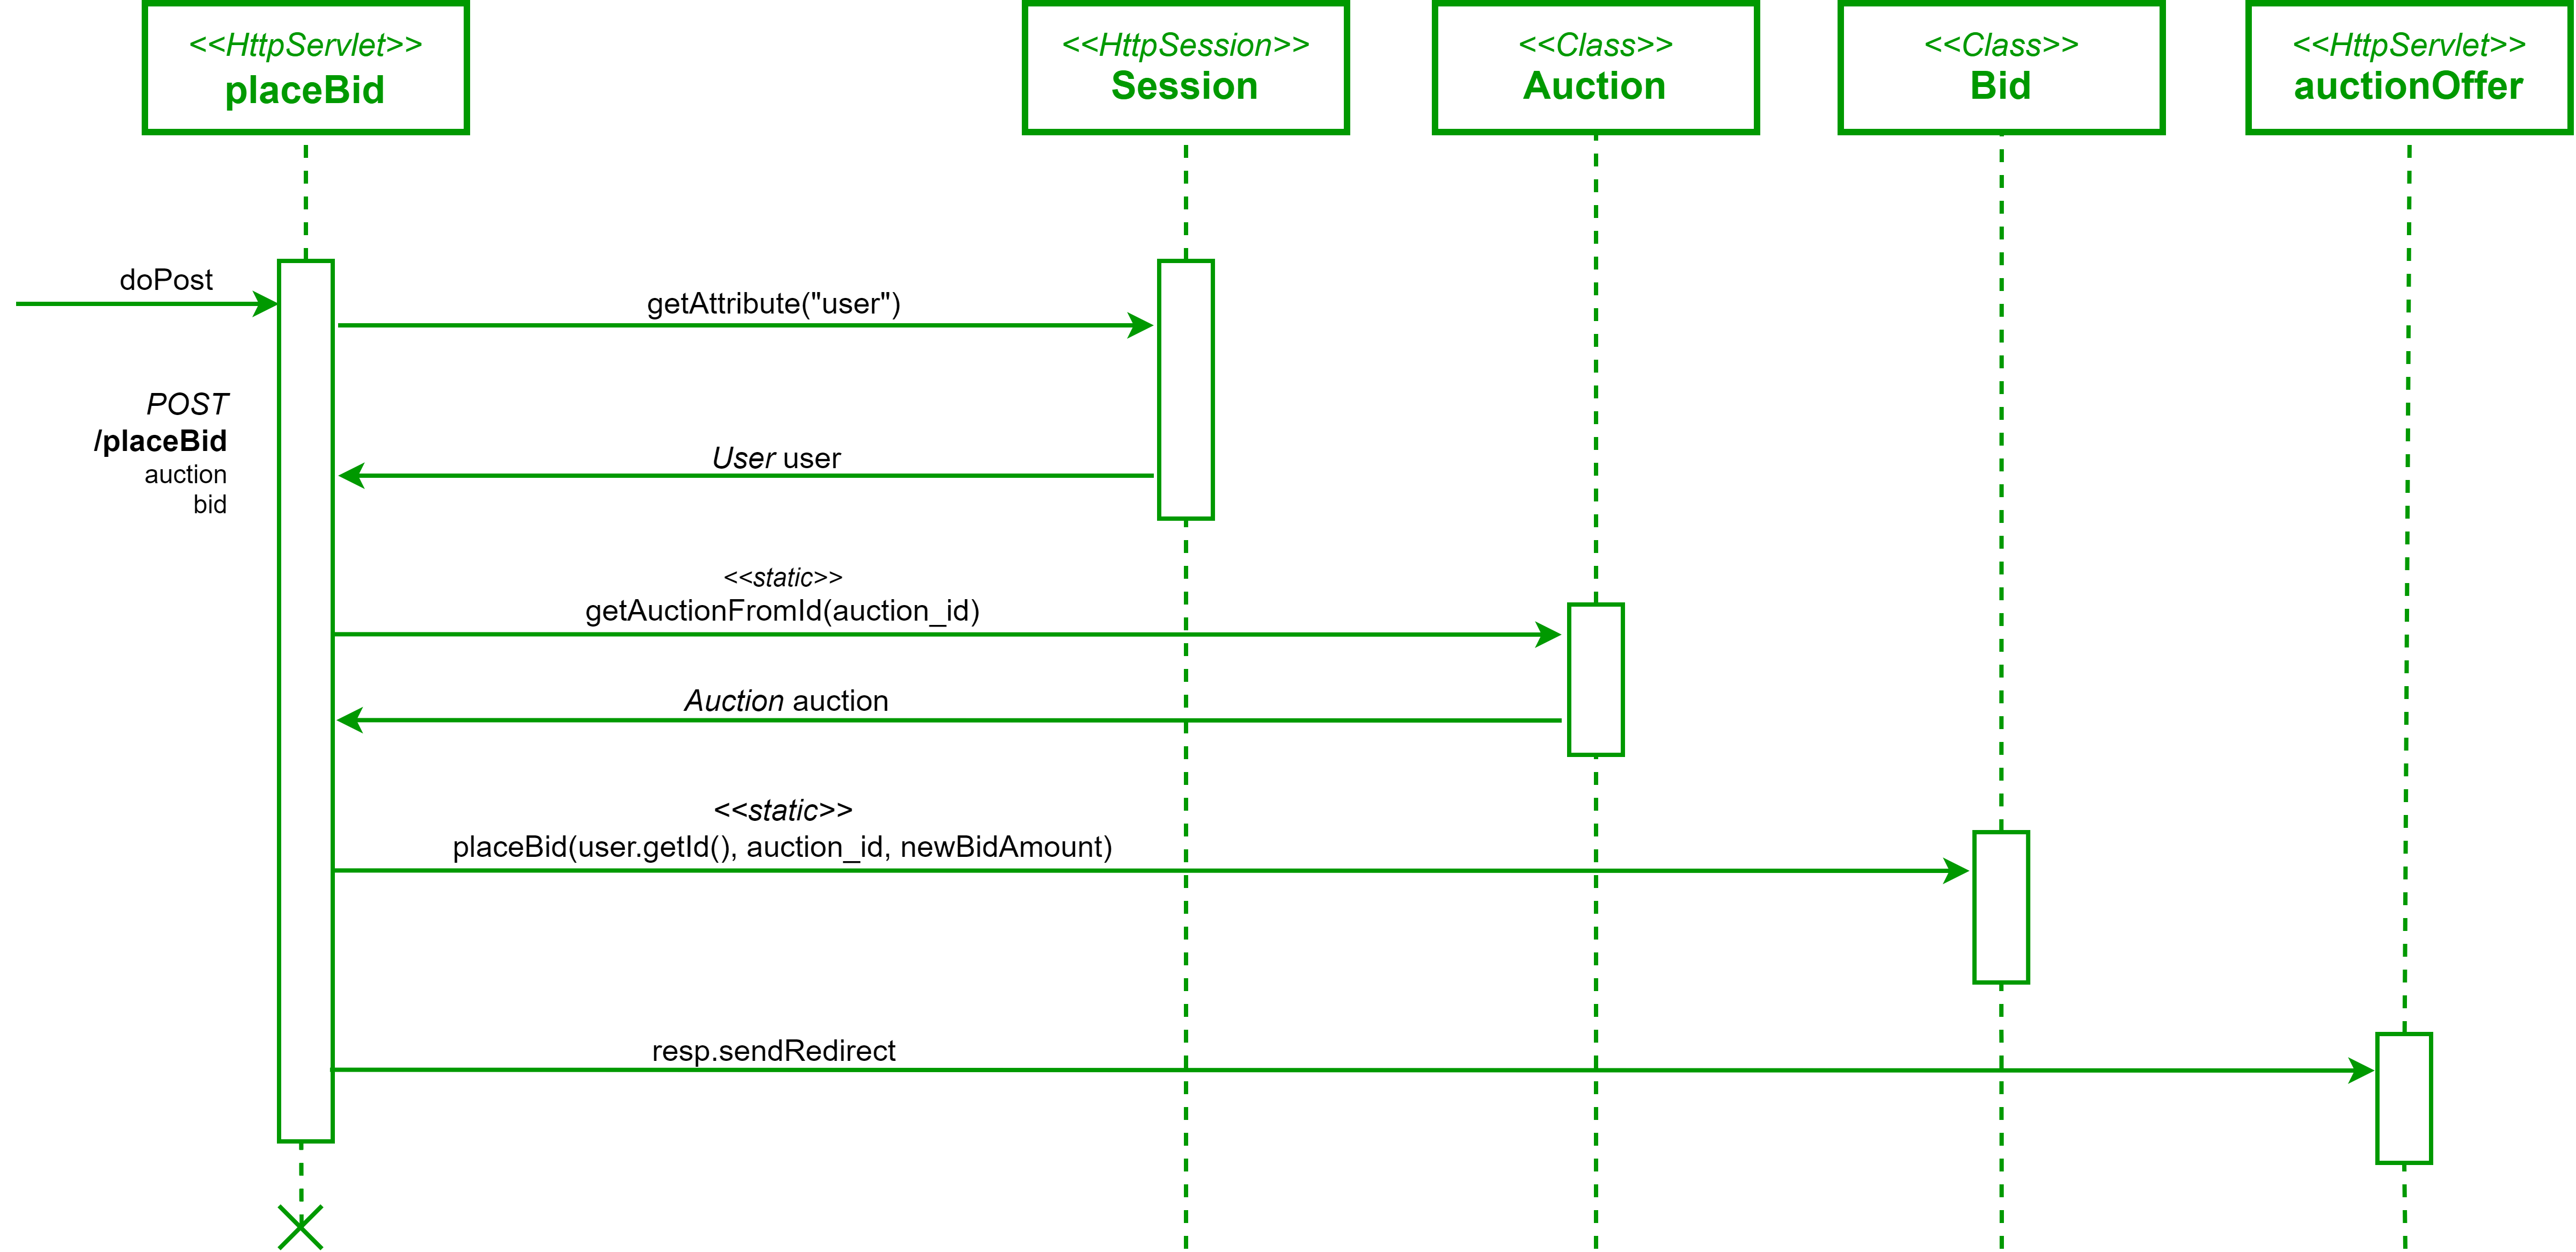
\includegraphics[width=1.15\textwidth]{SequenceDiagrams/TIW-placeBid.png}}
			\phantom{.}\\
			
			\subsubsection{A user requests the SELL page}
			\phantom{.}\\
			\noindent \makebox[\textwidth]{
				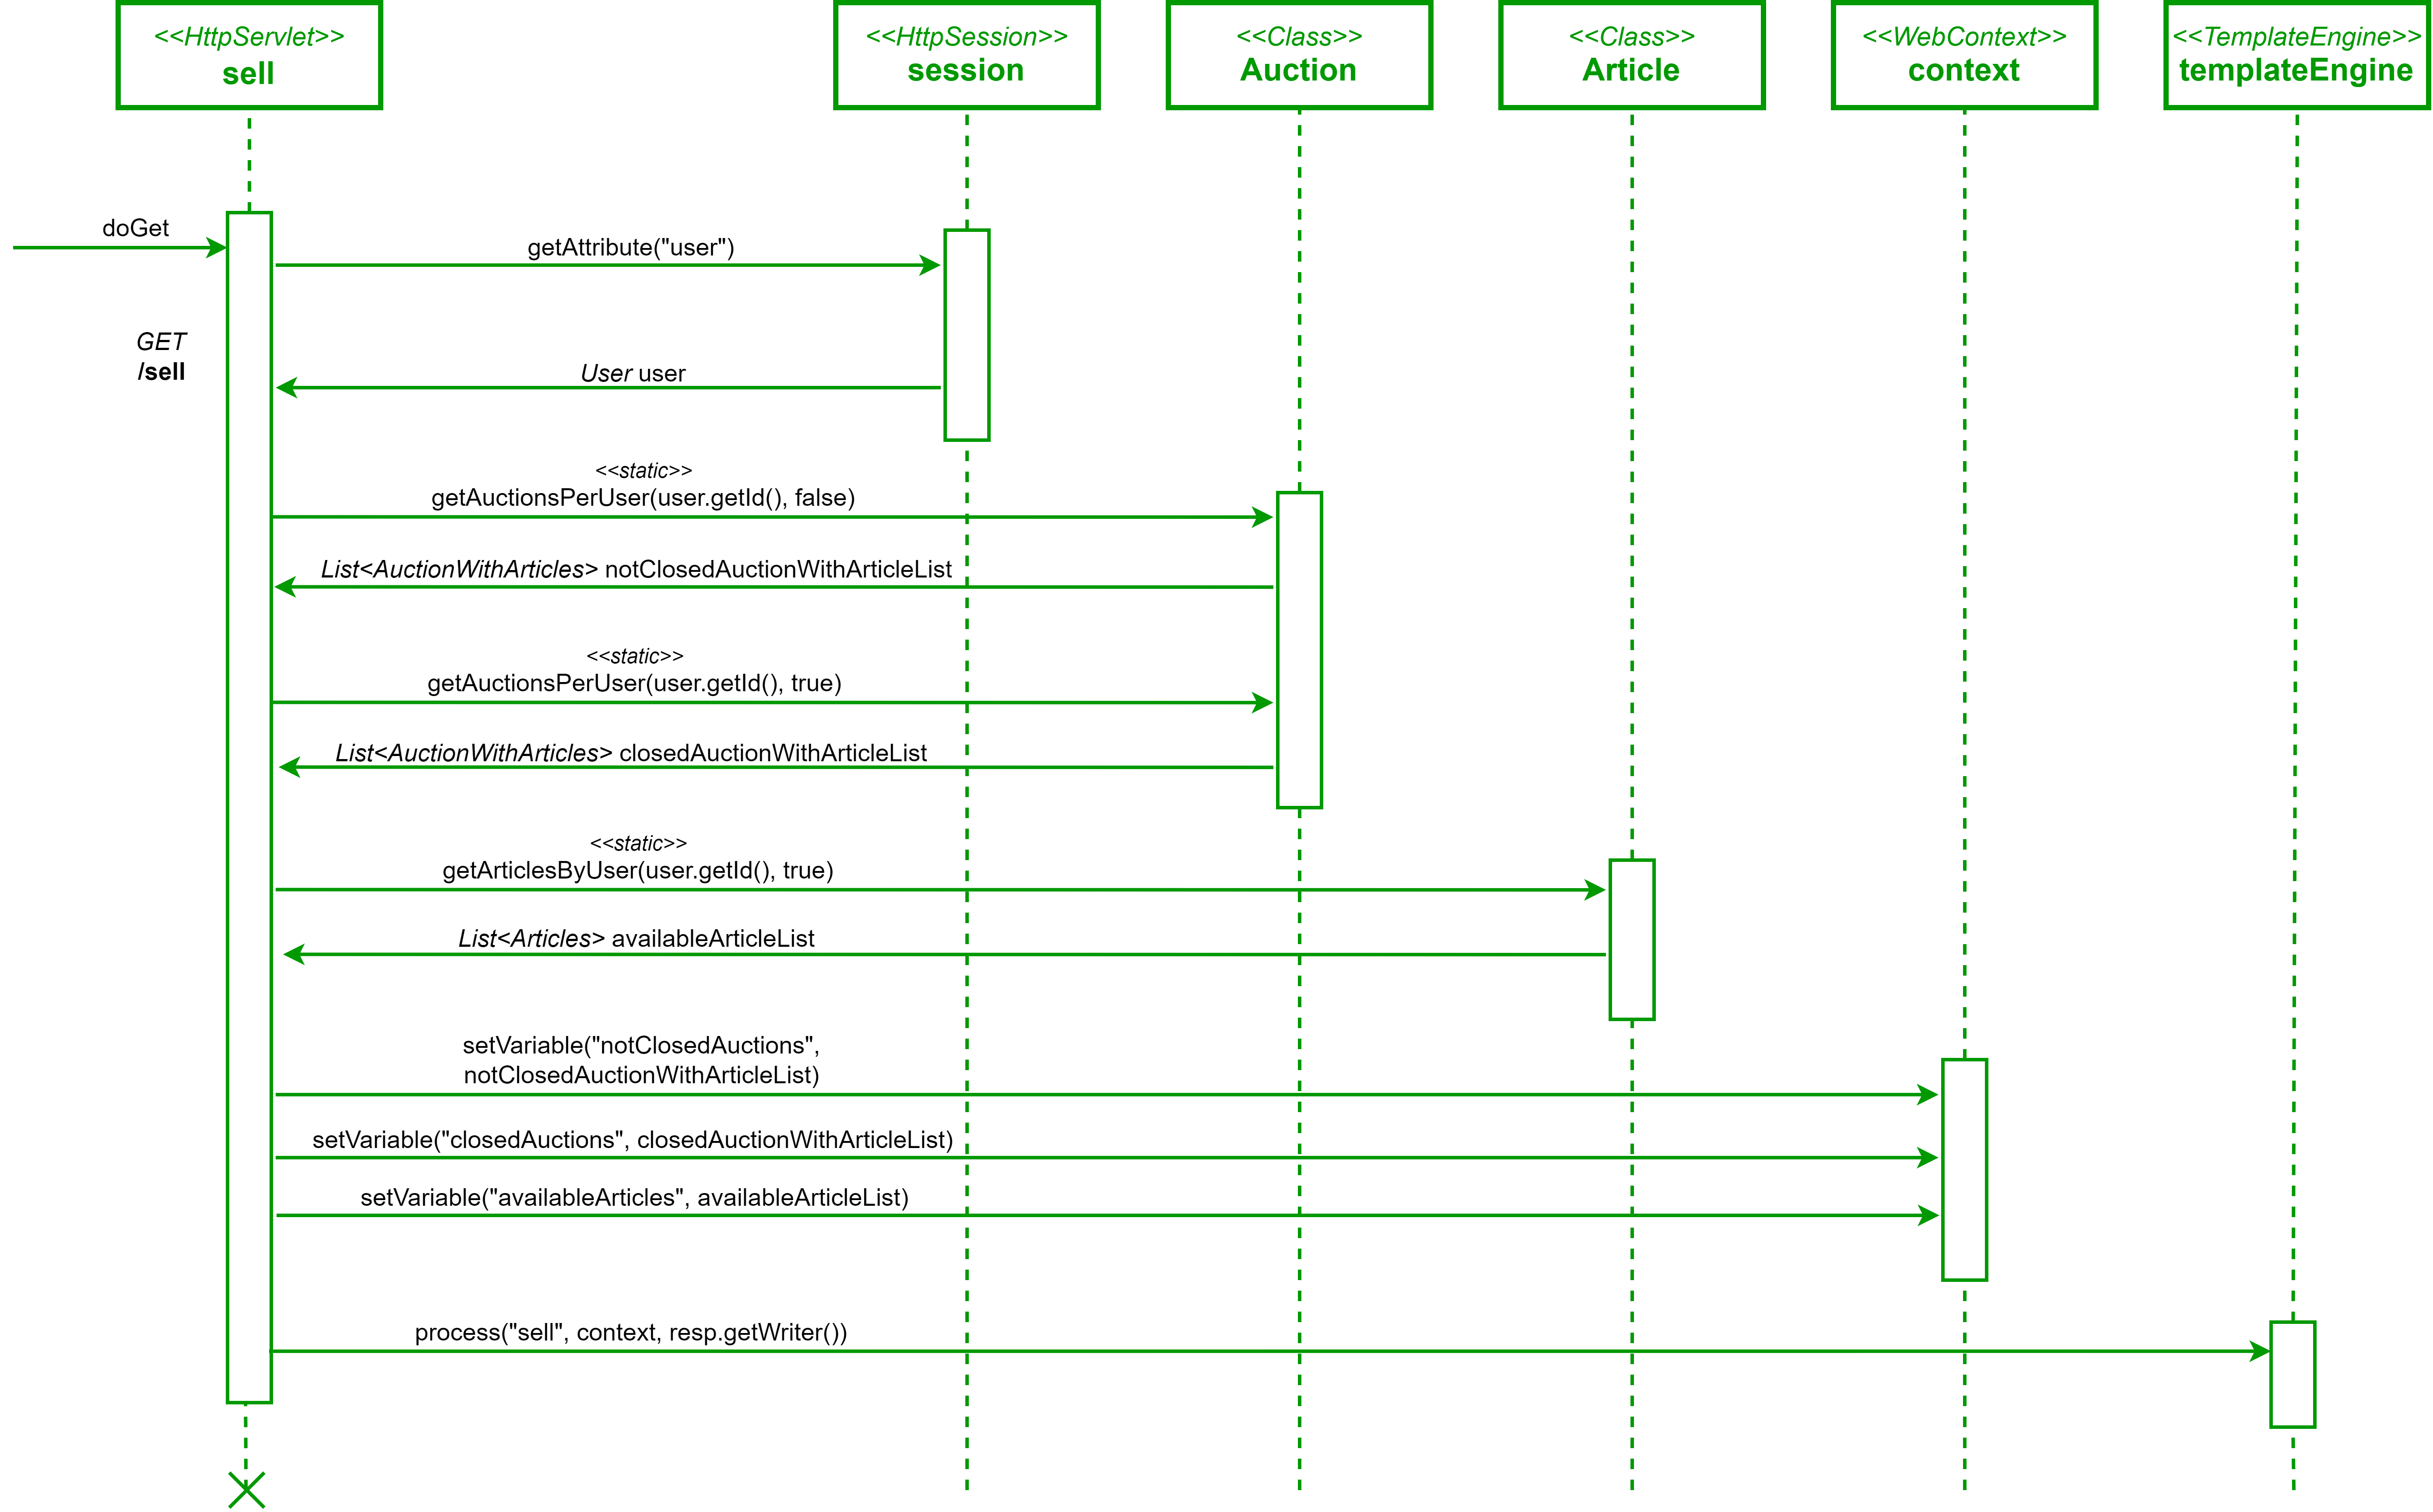
\includegraphics[width=1.2\textwidth]{SequenceDiagrams/TIW-sell.png}}	
			\phantom{.}\\
			\newpage
			\subsubsection{A user (the owner) requests the details page of their auction}
			\phantom{.}\\
			\noindent \makebox[\textwidth]{
				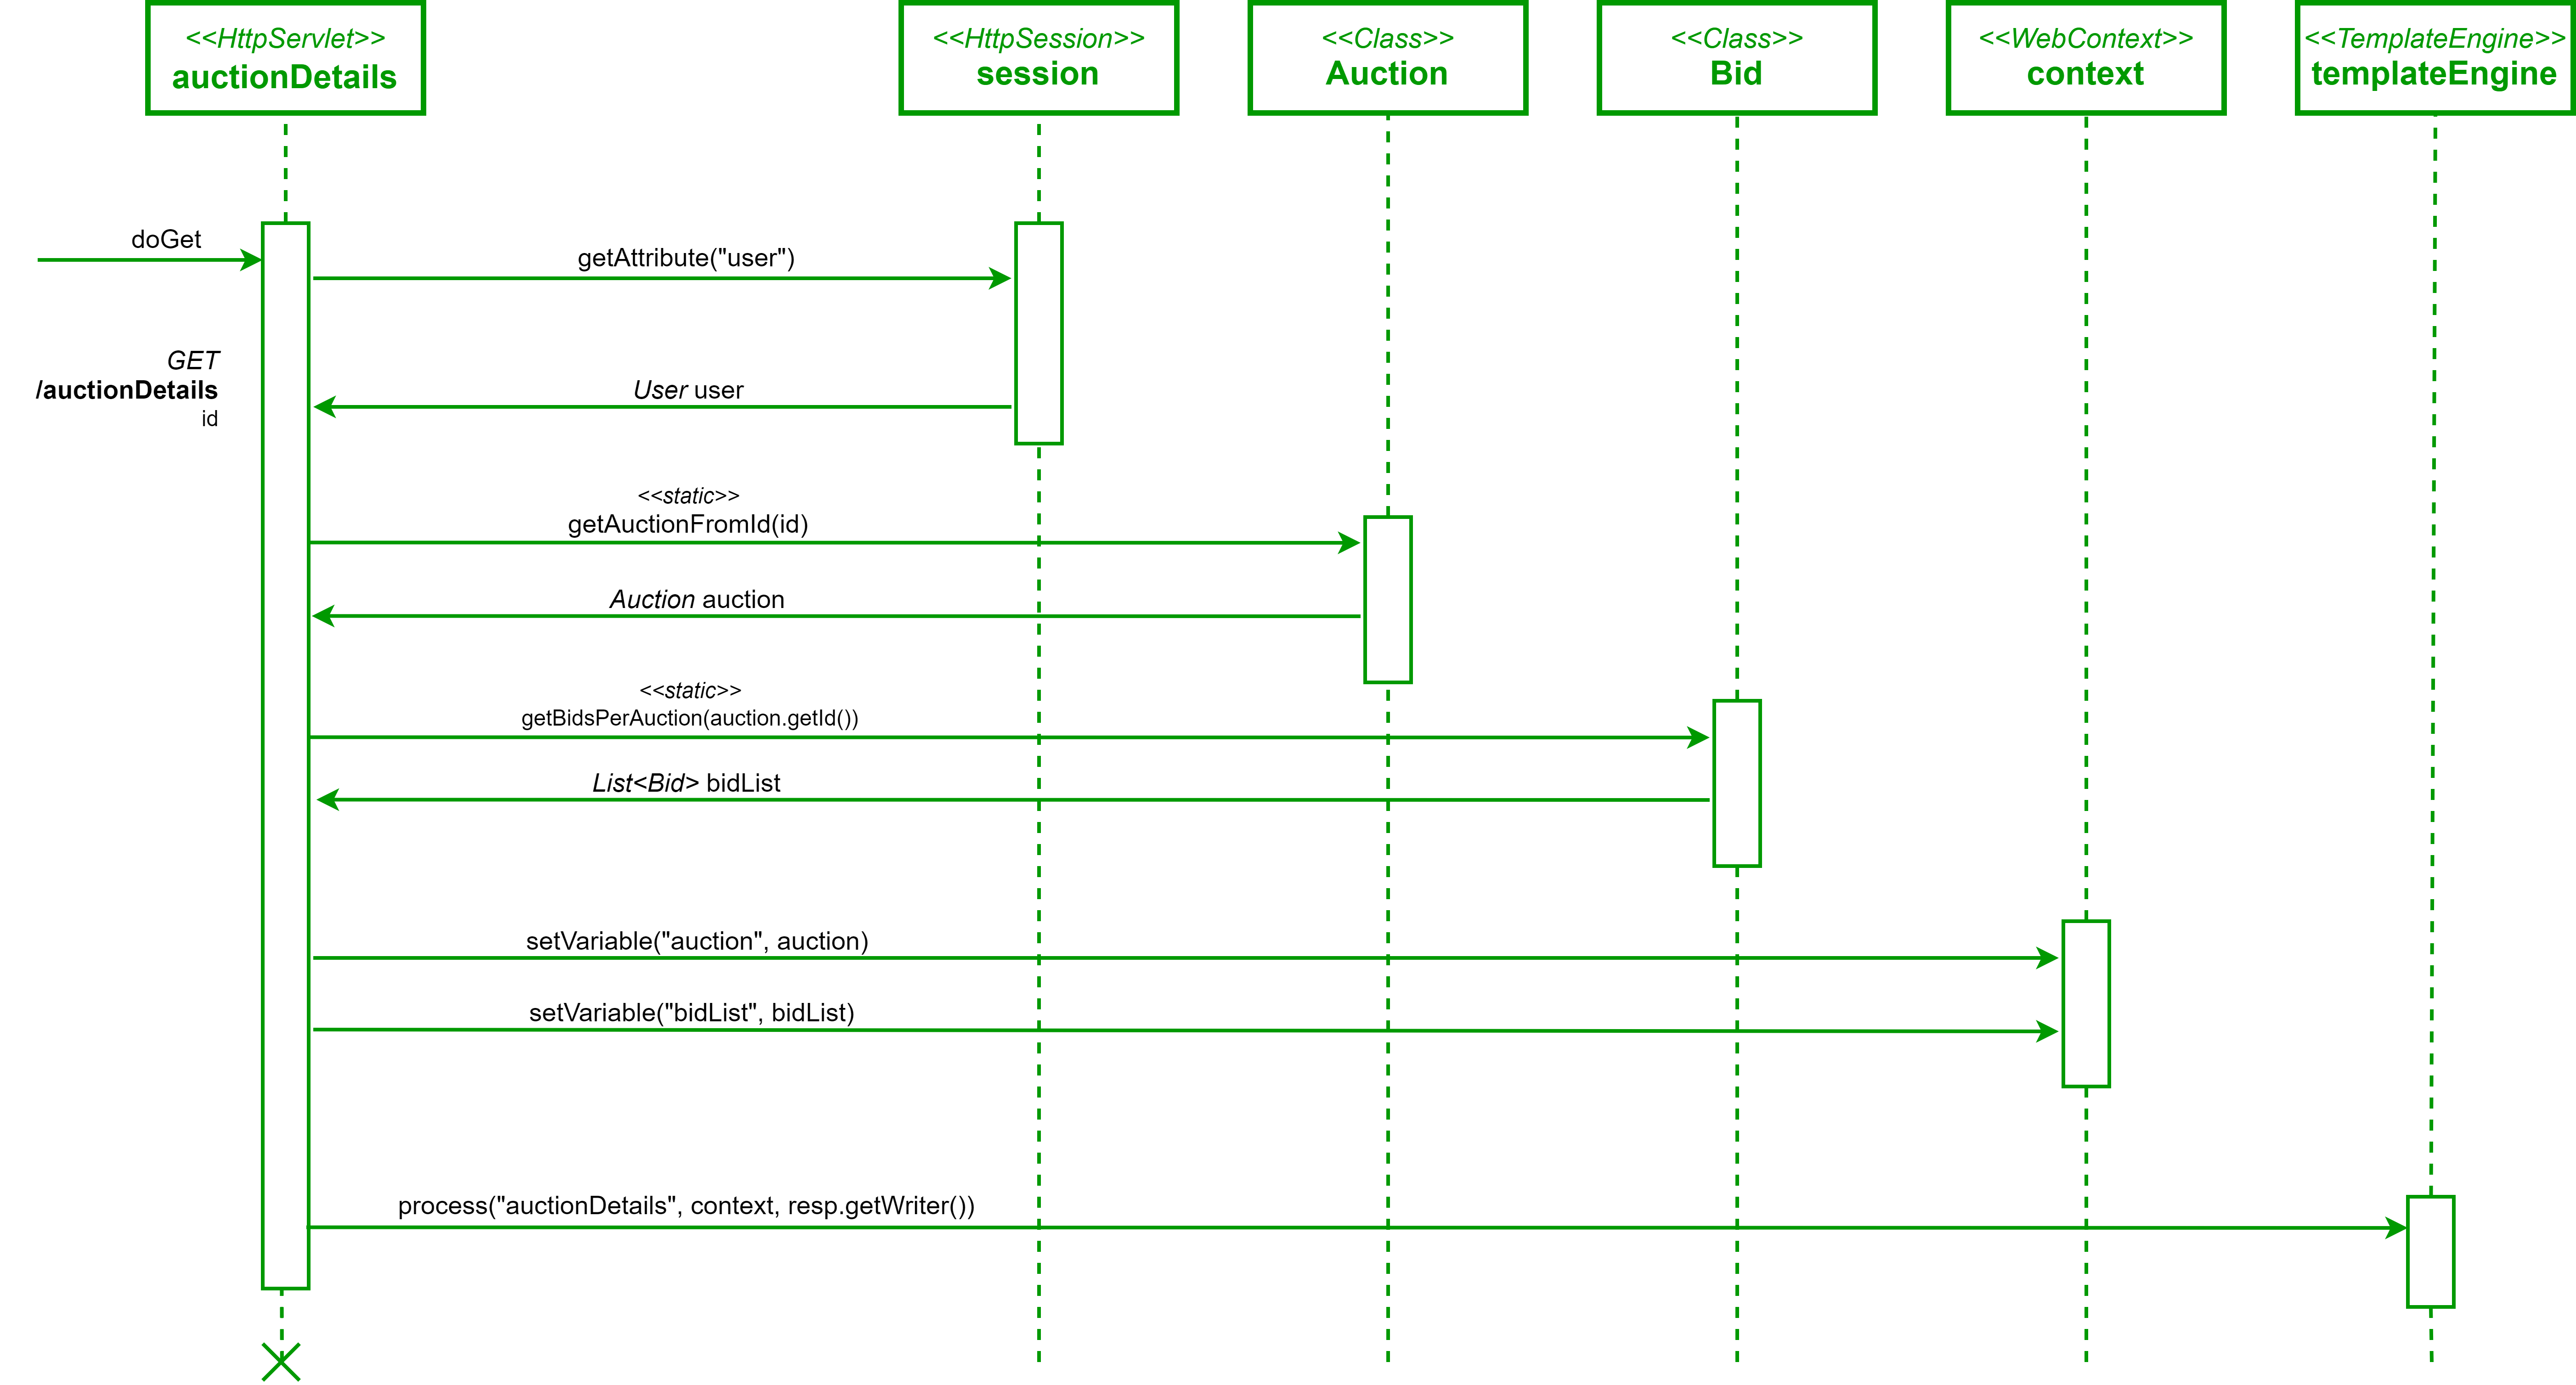
\includegraphics[width=1.3\textwidth]{SequenceDiagrams/TIW-auctionDetails.png}}	
			\phantom{.}\\
			\subsubsection{A user uploads a new article}
			\phantom{.}\\
			\noindent \makebox[\textwidth]{
				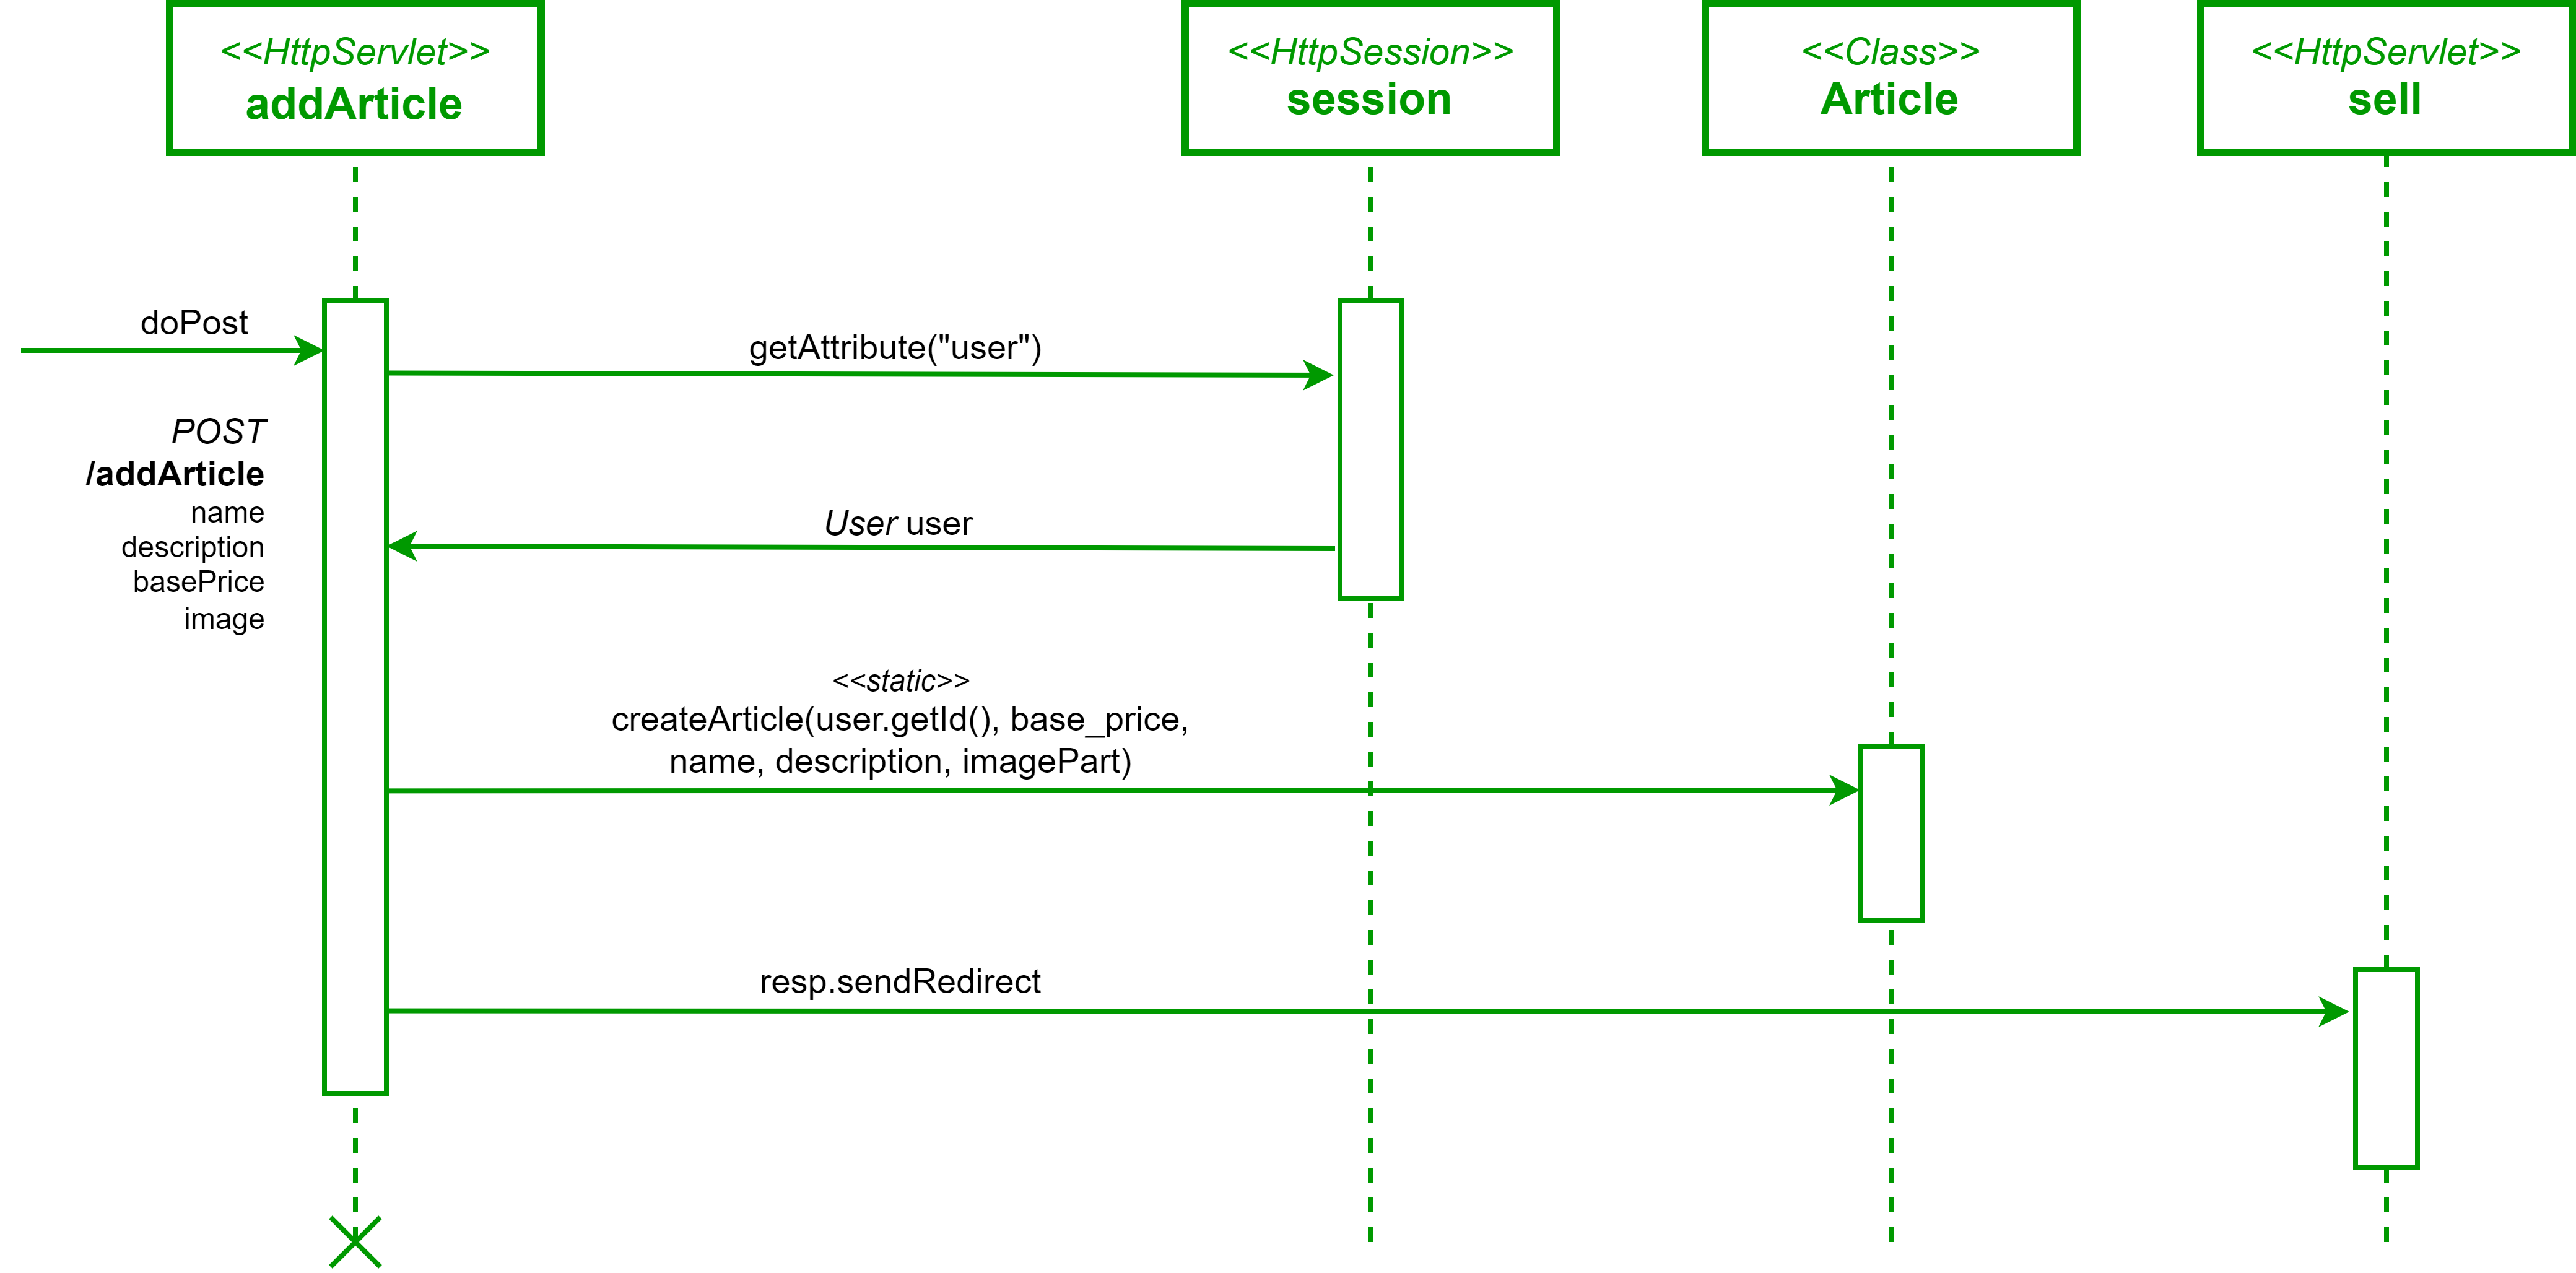
\includegraphics[width=1.1\textwidth]{SequenceDiagrams/TIW-addArticle.png}}	
			\phantom{.}\\
			\newpage
			\subsubsection{A user creates a new auction}
			\phantom{.}\\
			\noindent \makebox[\textwidth]{
				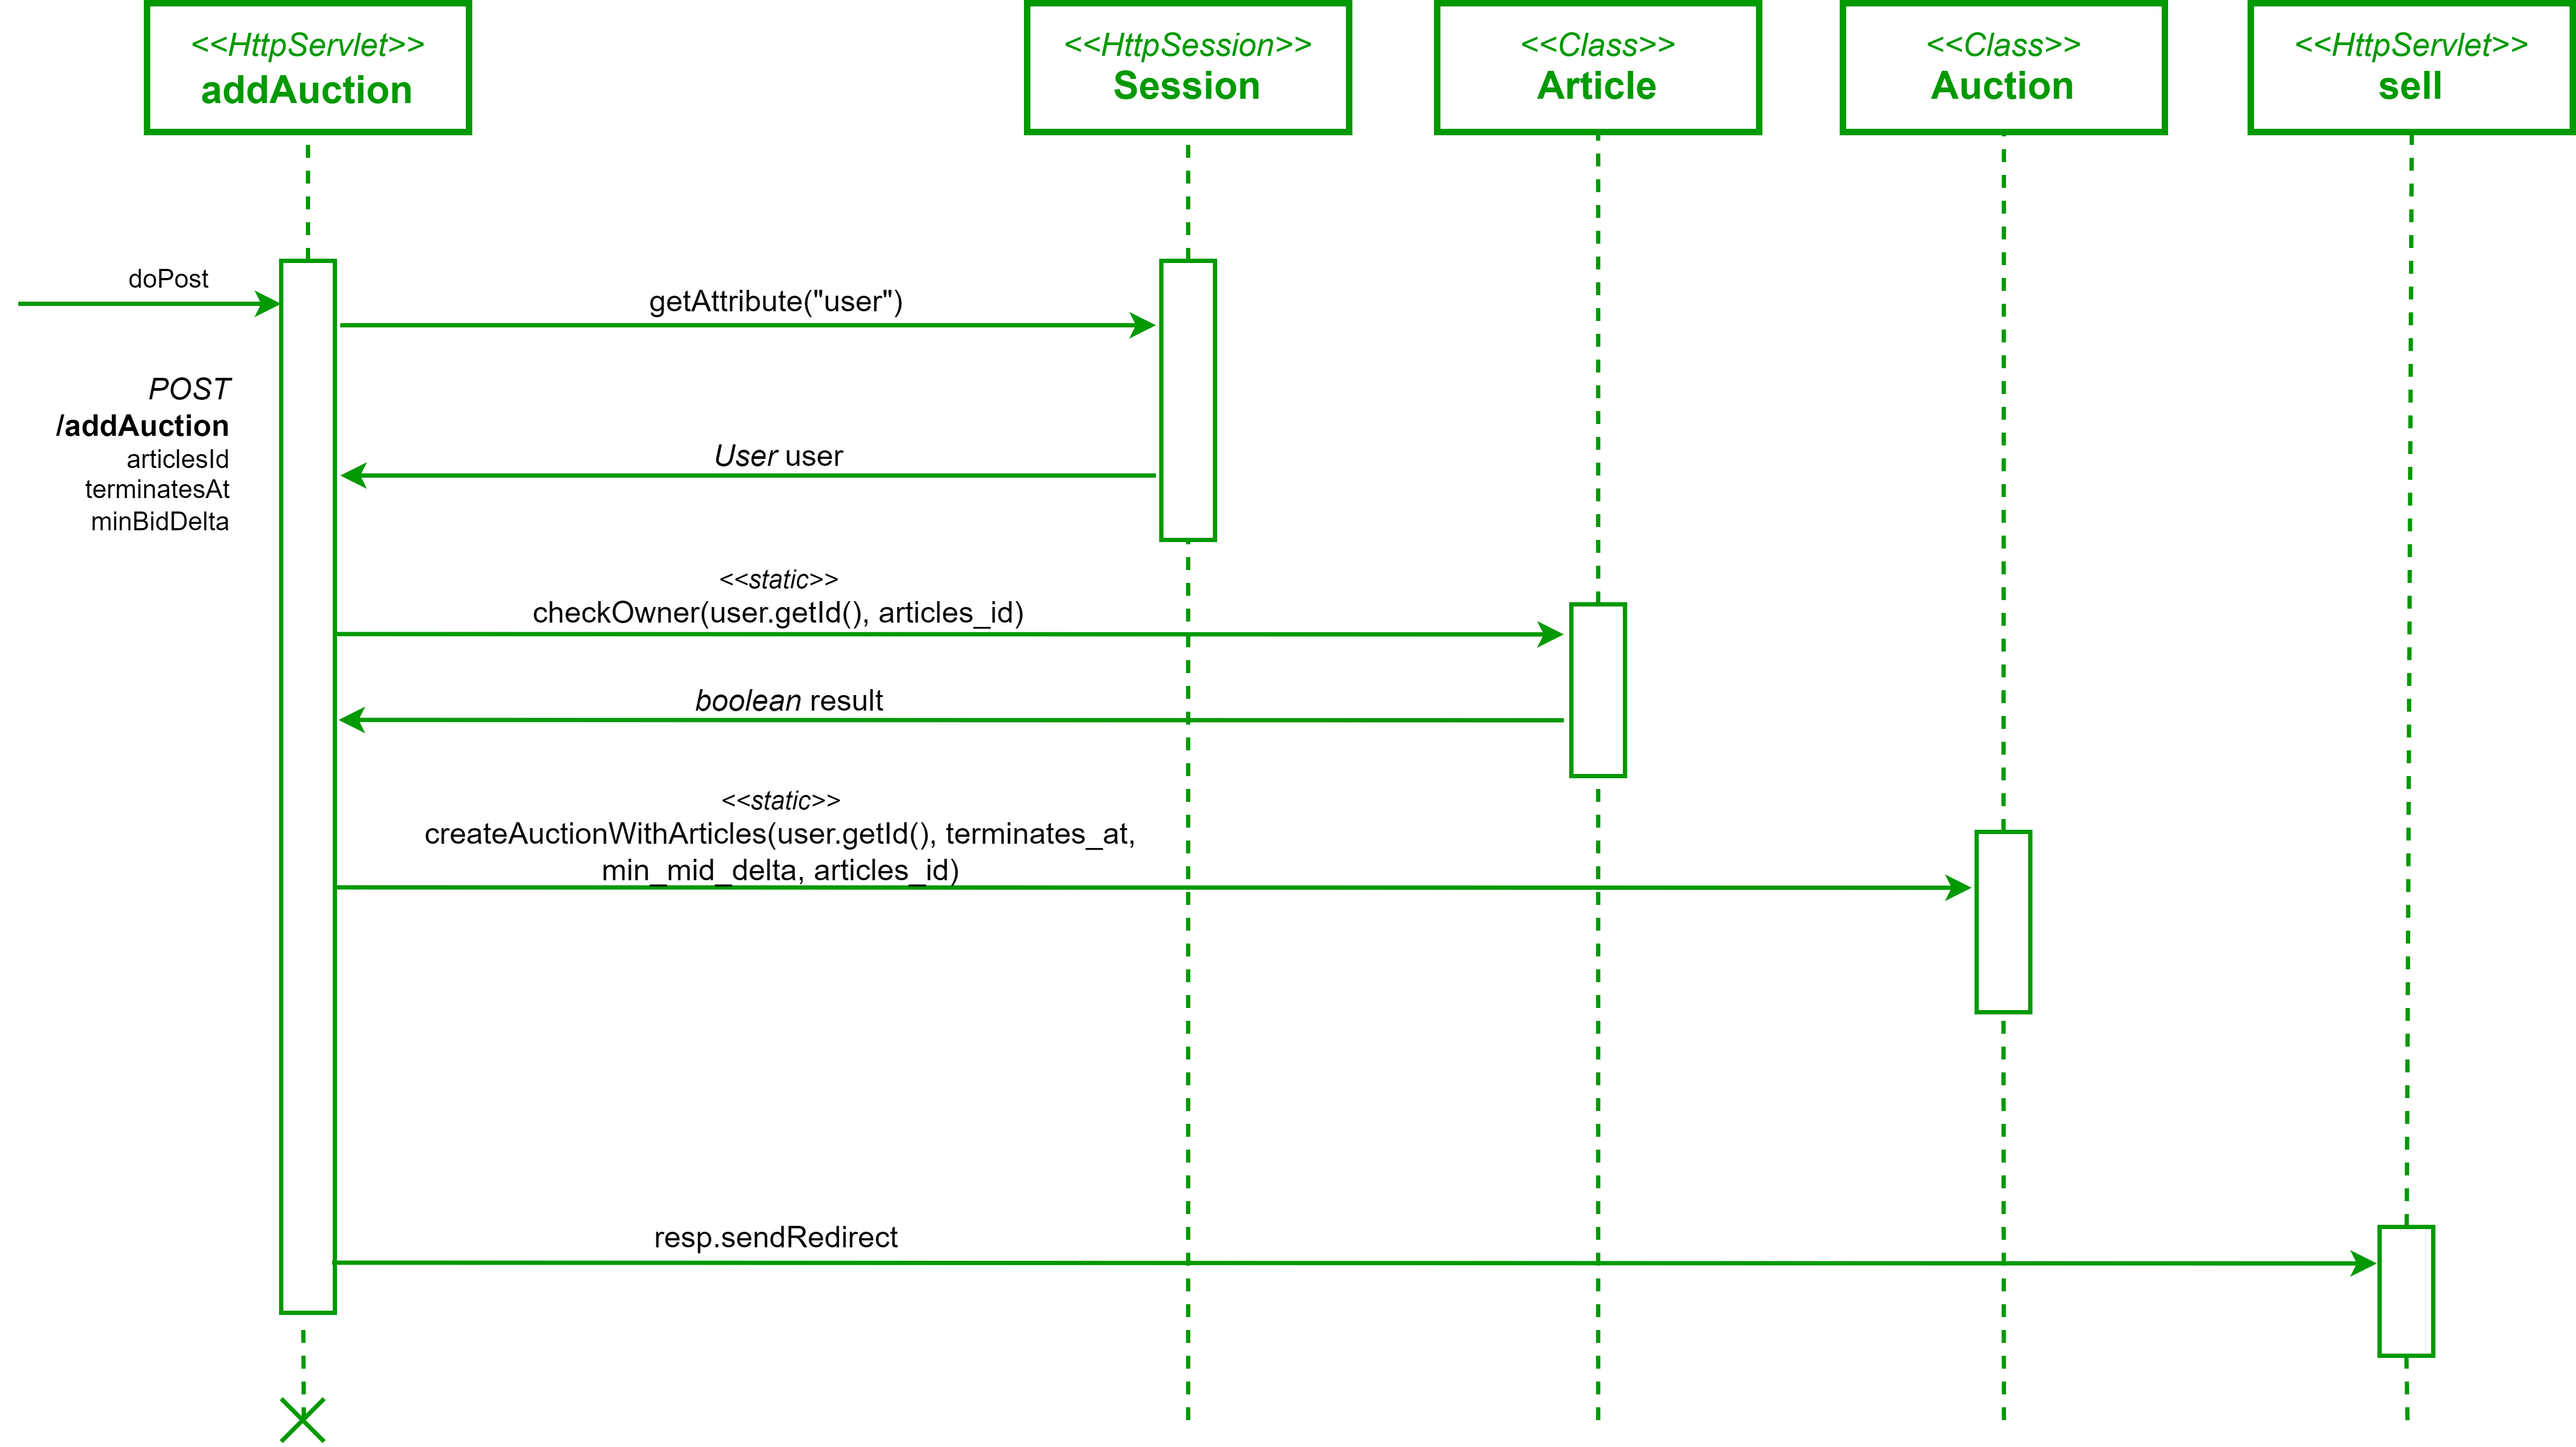
\includegraphics[width=1.3\textwidth]{SequenceDiagrams/TIW-addAuction.png}}	
			\phantom{.}\\
			\subsubsection{A user (the owner) closes a finished auction}
			\phantom{.}\\
			\noindent \makebox[\textwidth]{
				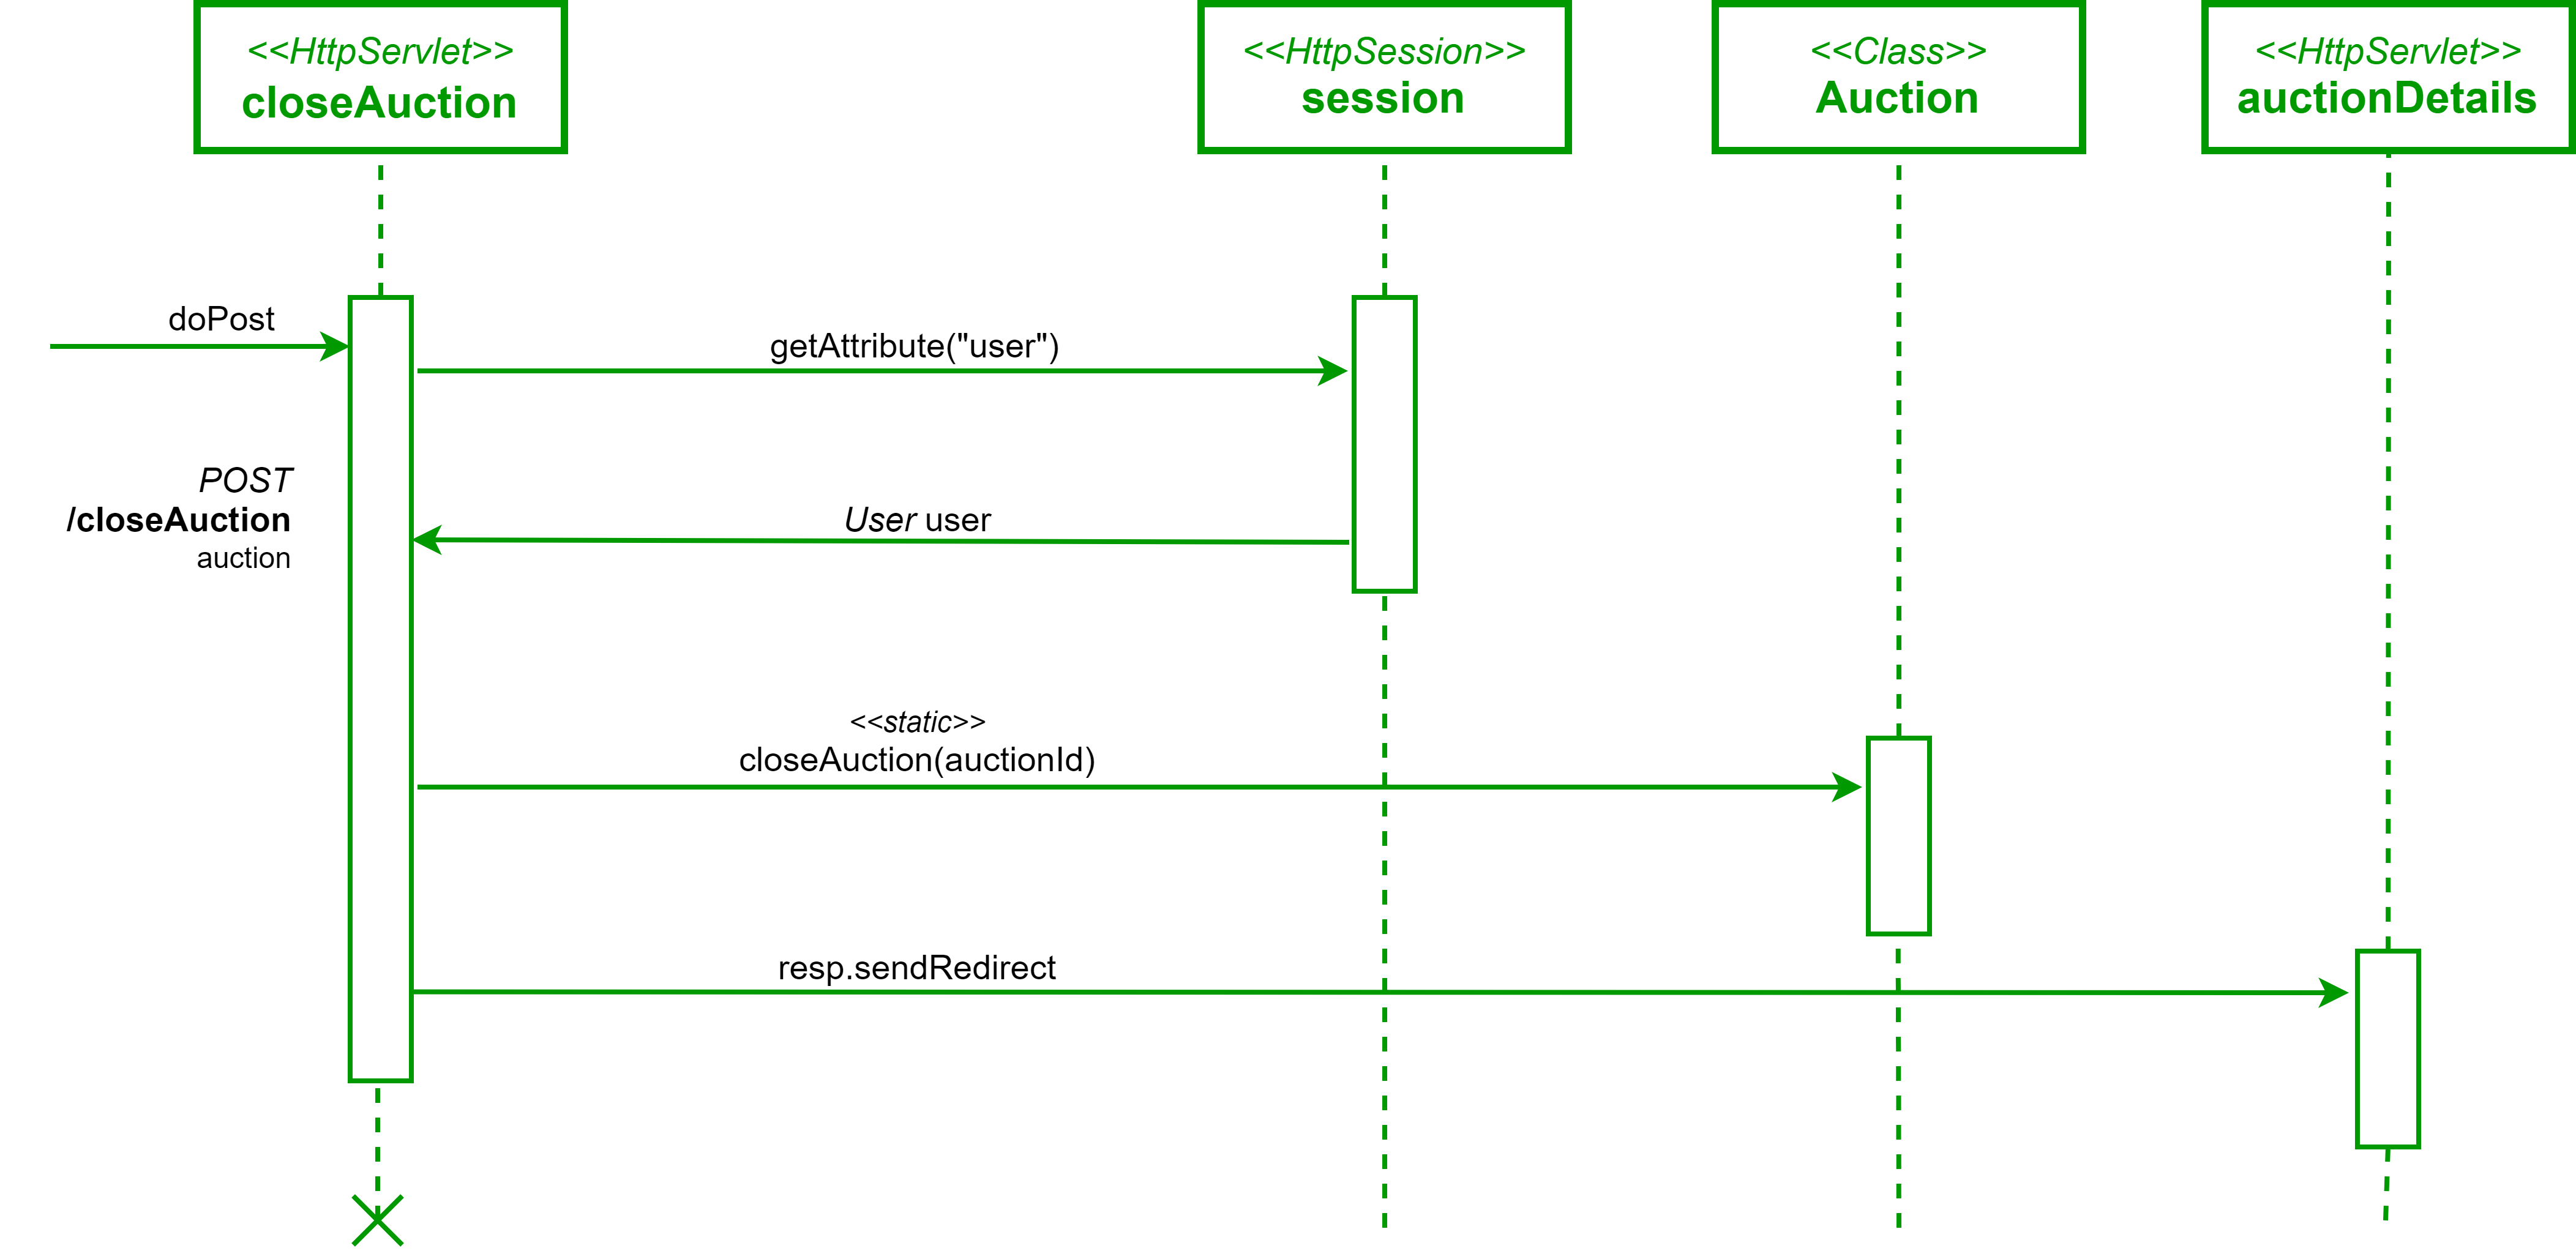
\includegraphics[width=1.1\textwidth]{SequenceDiagrams/TIW-closeAuction.png}}					
			\phantom{.}\\
			\newpage			
		\section[RIA - Application Design]{Application Design for the JavaScript Version}
			\subsection{Page Structure}
				\noindent \makebox[\textwidth]{
					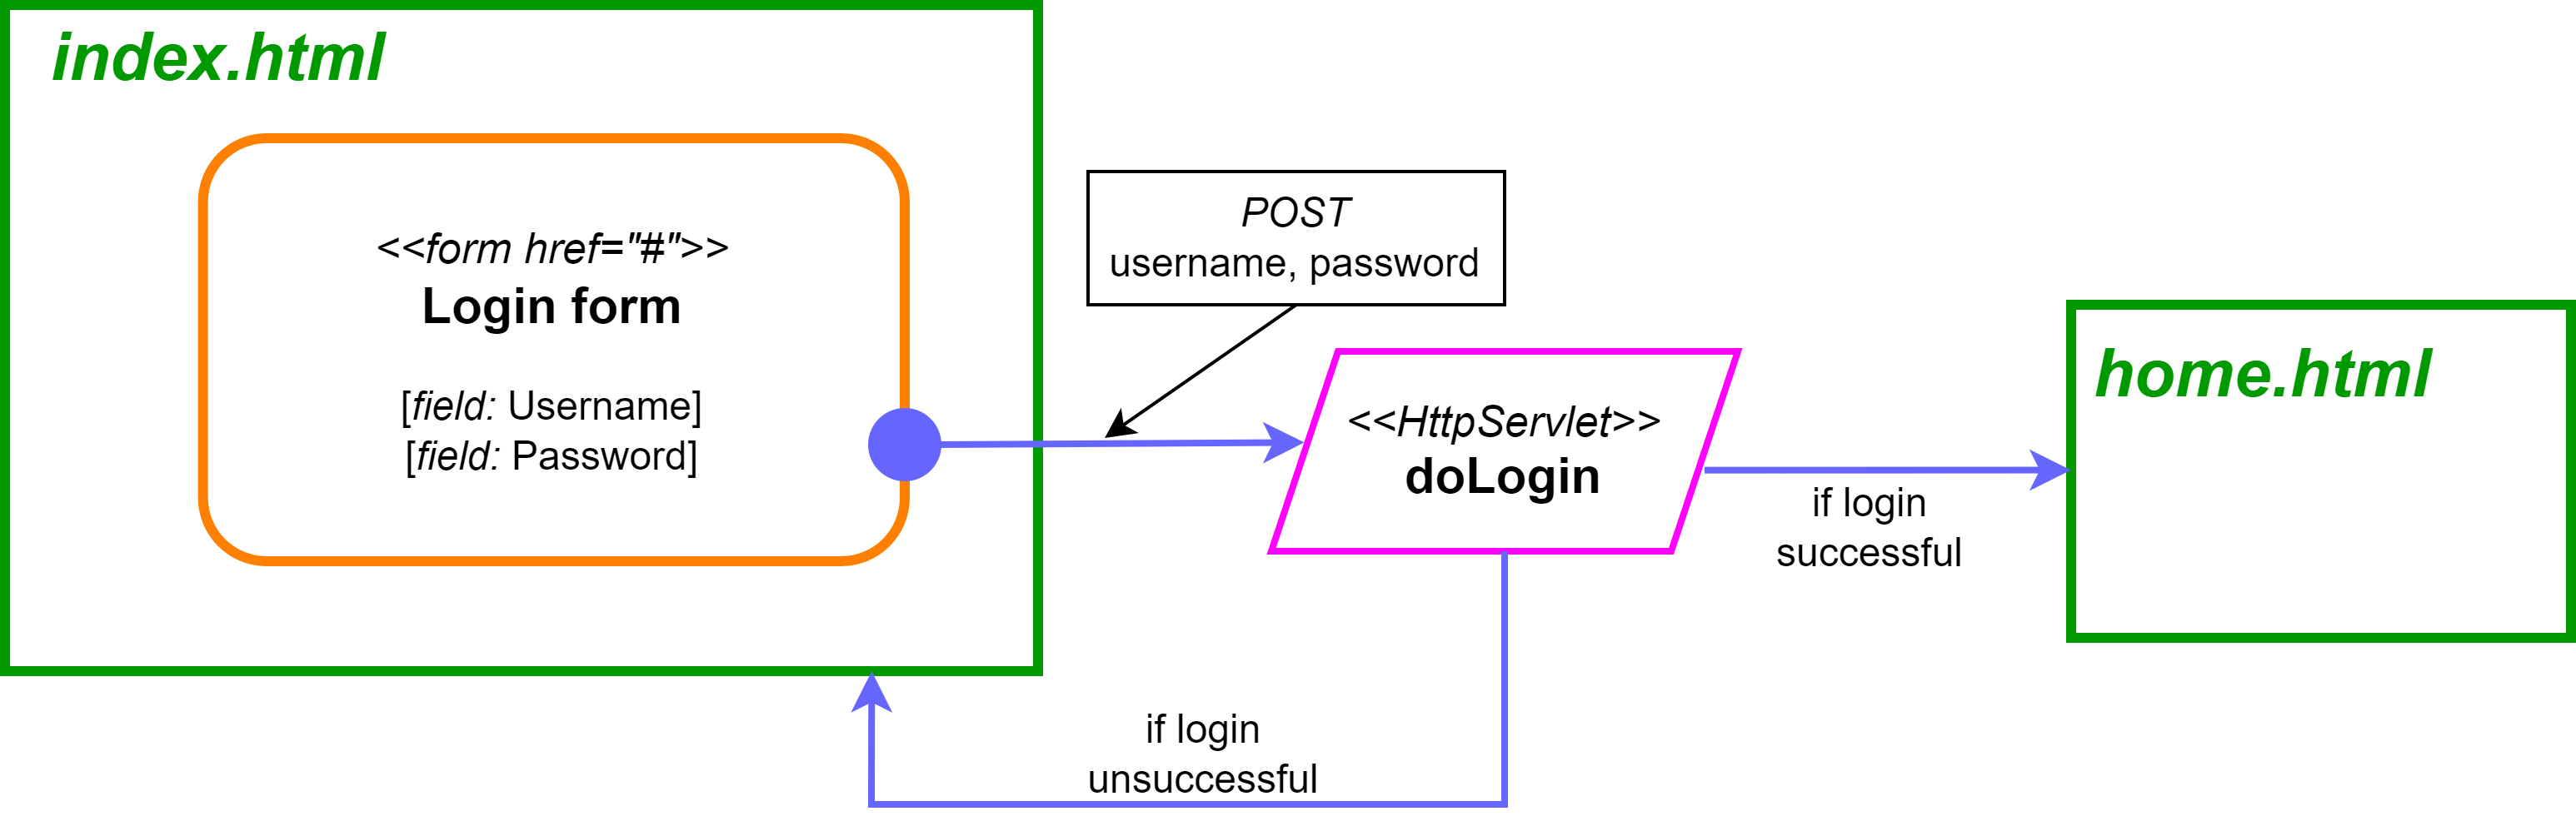
\includegraphics[width=1\textwidth]{RIA-design/TIWRIA-login.png}}
				\phantom{.}\\
				\noindent \makebox[\textwidth]{
					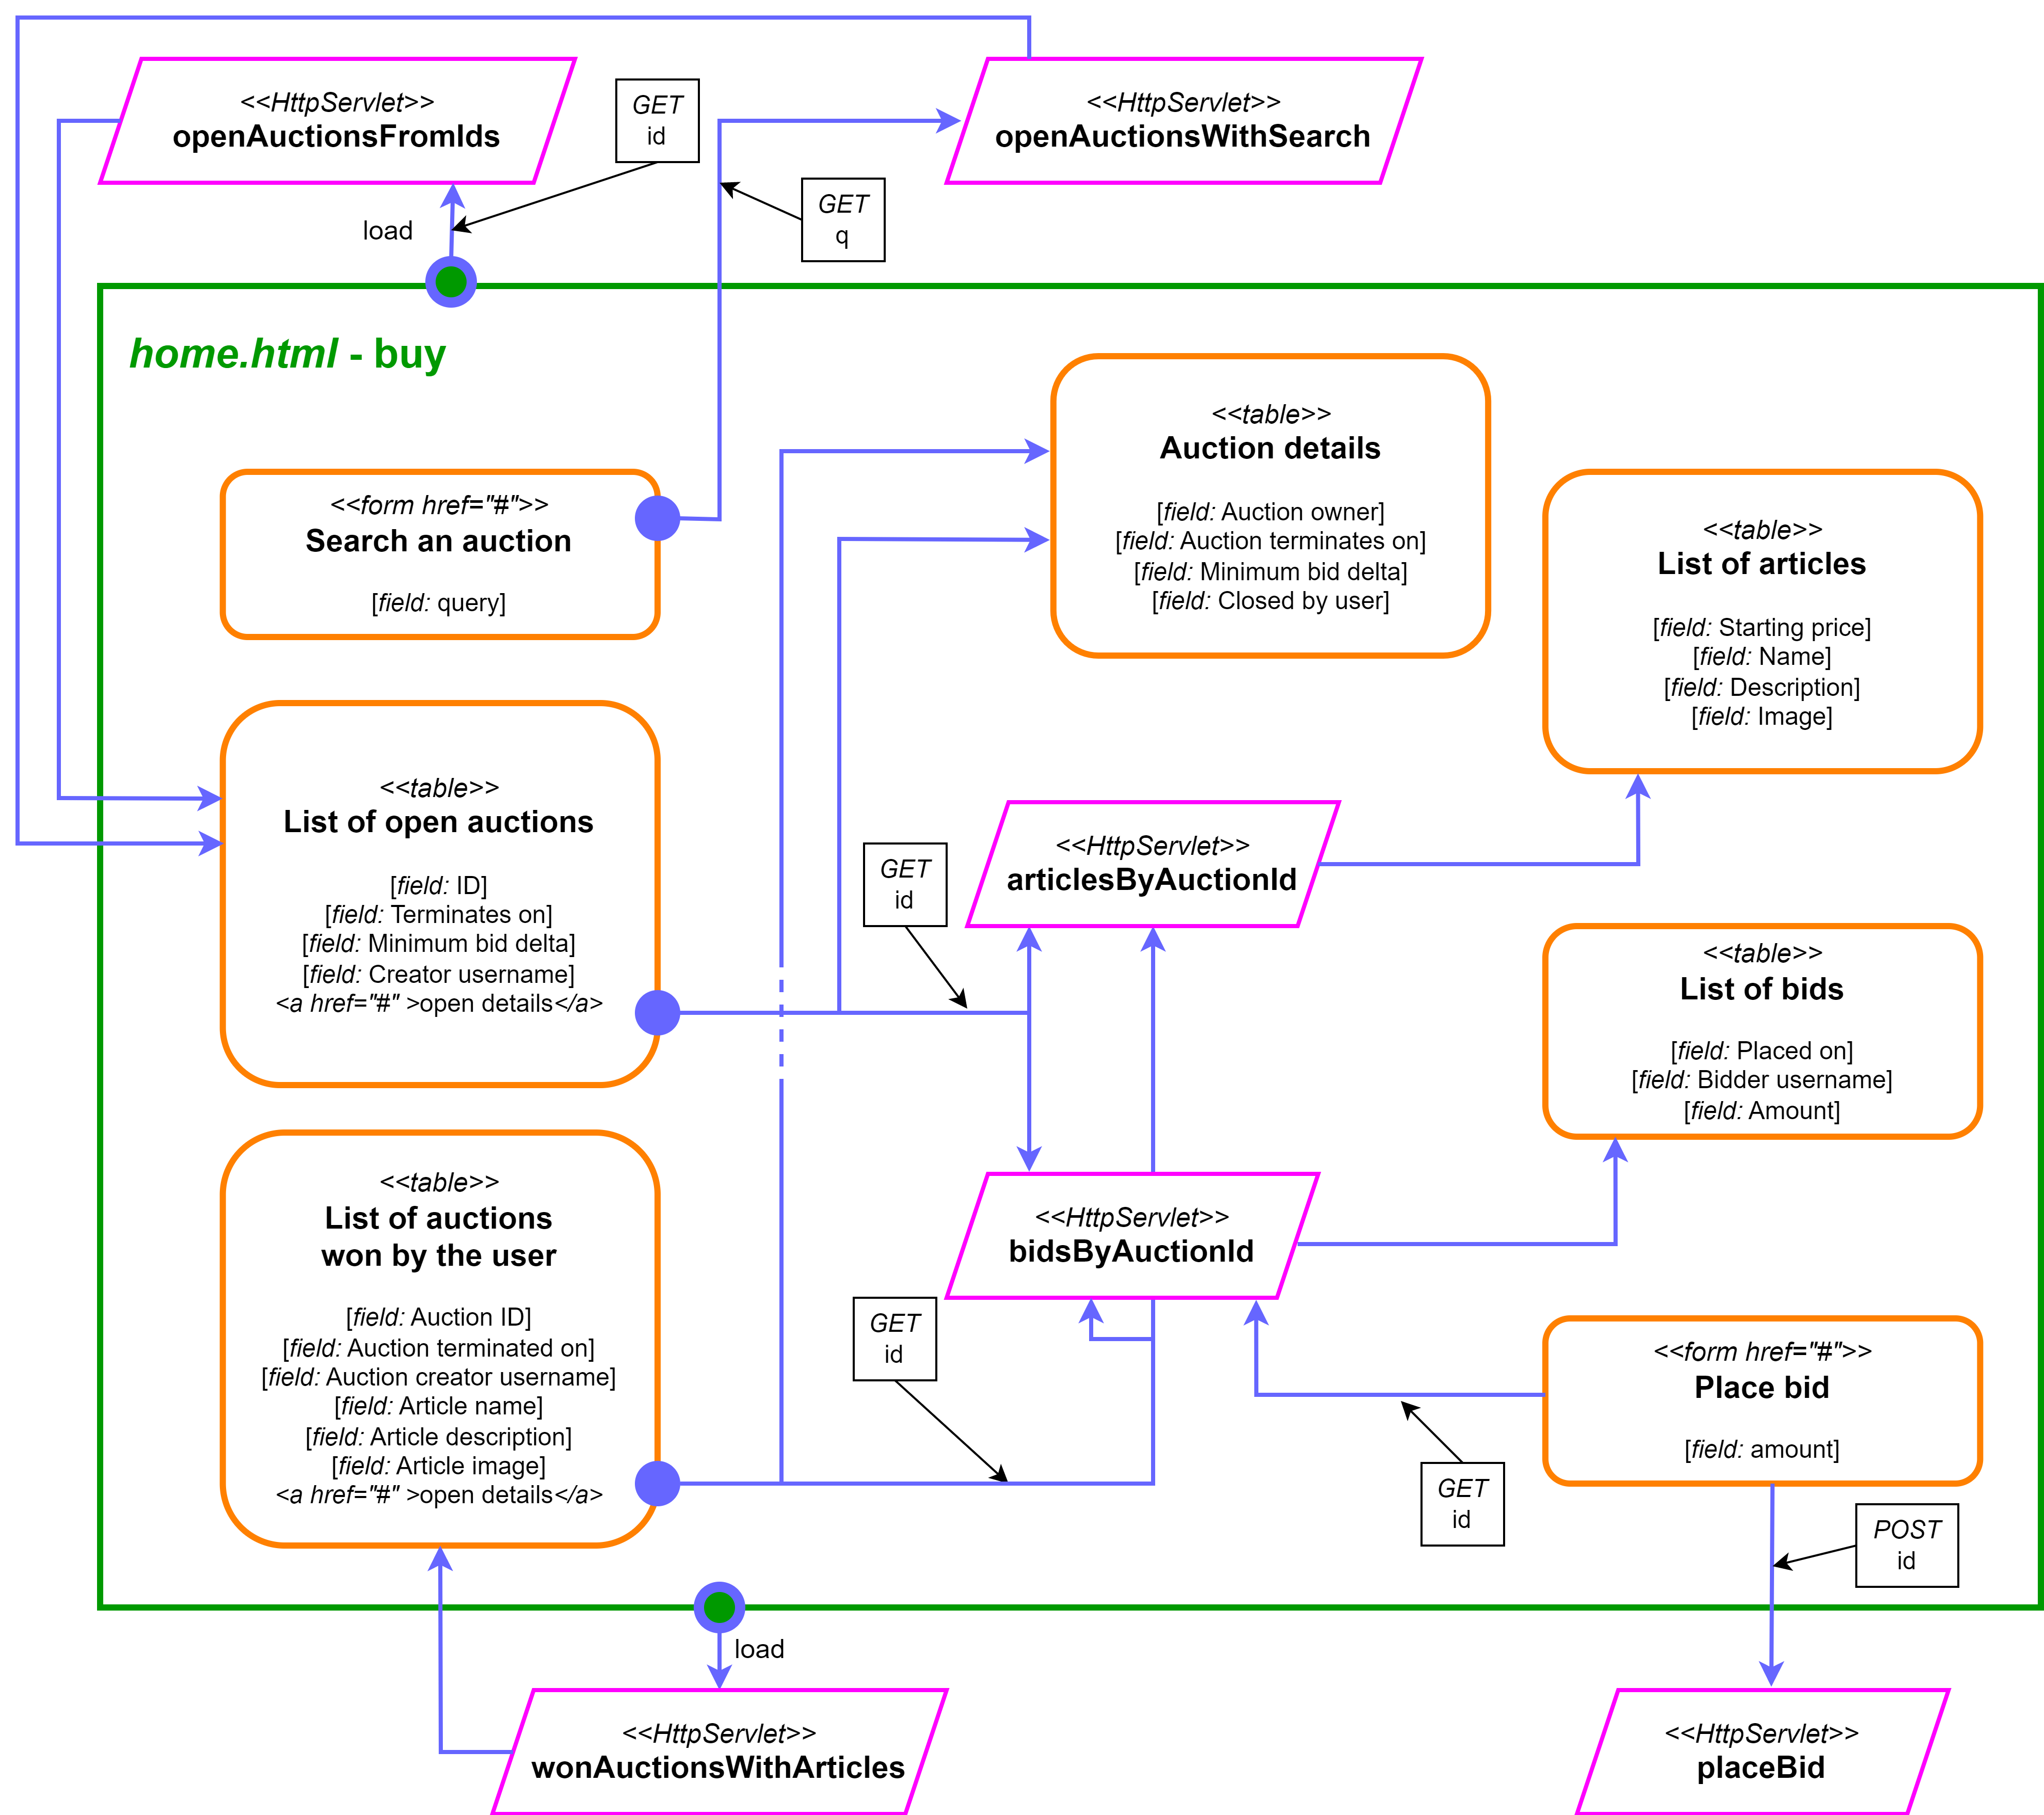
\includegraphics[width=1.2\textwidth]{RIA-design/TIWRIA-buy.png}}
				\newpage
				\noindent \makebox[\textwidth]{
					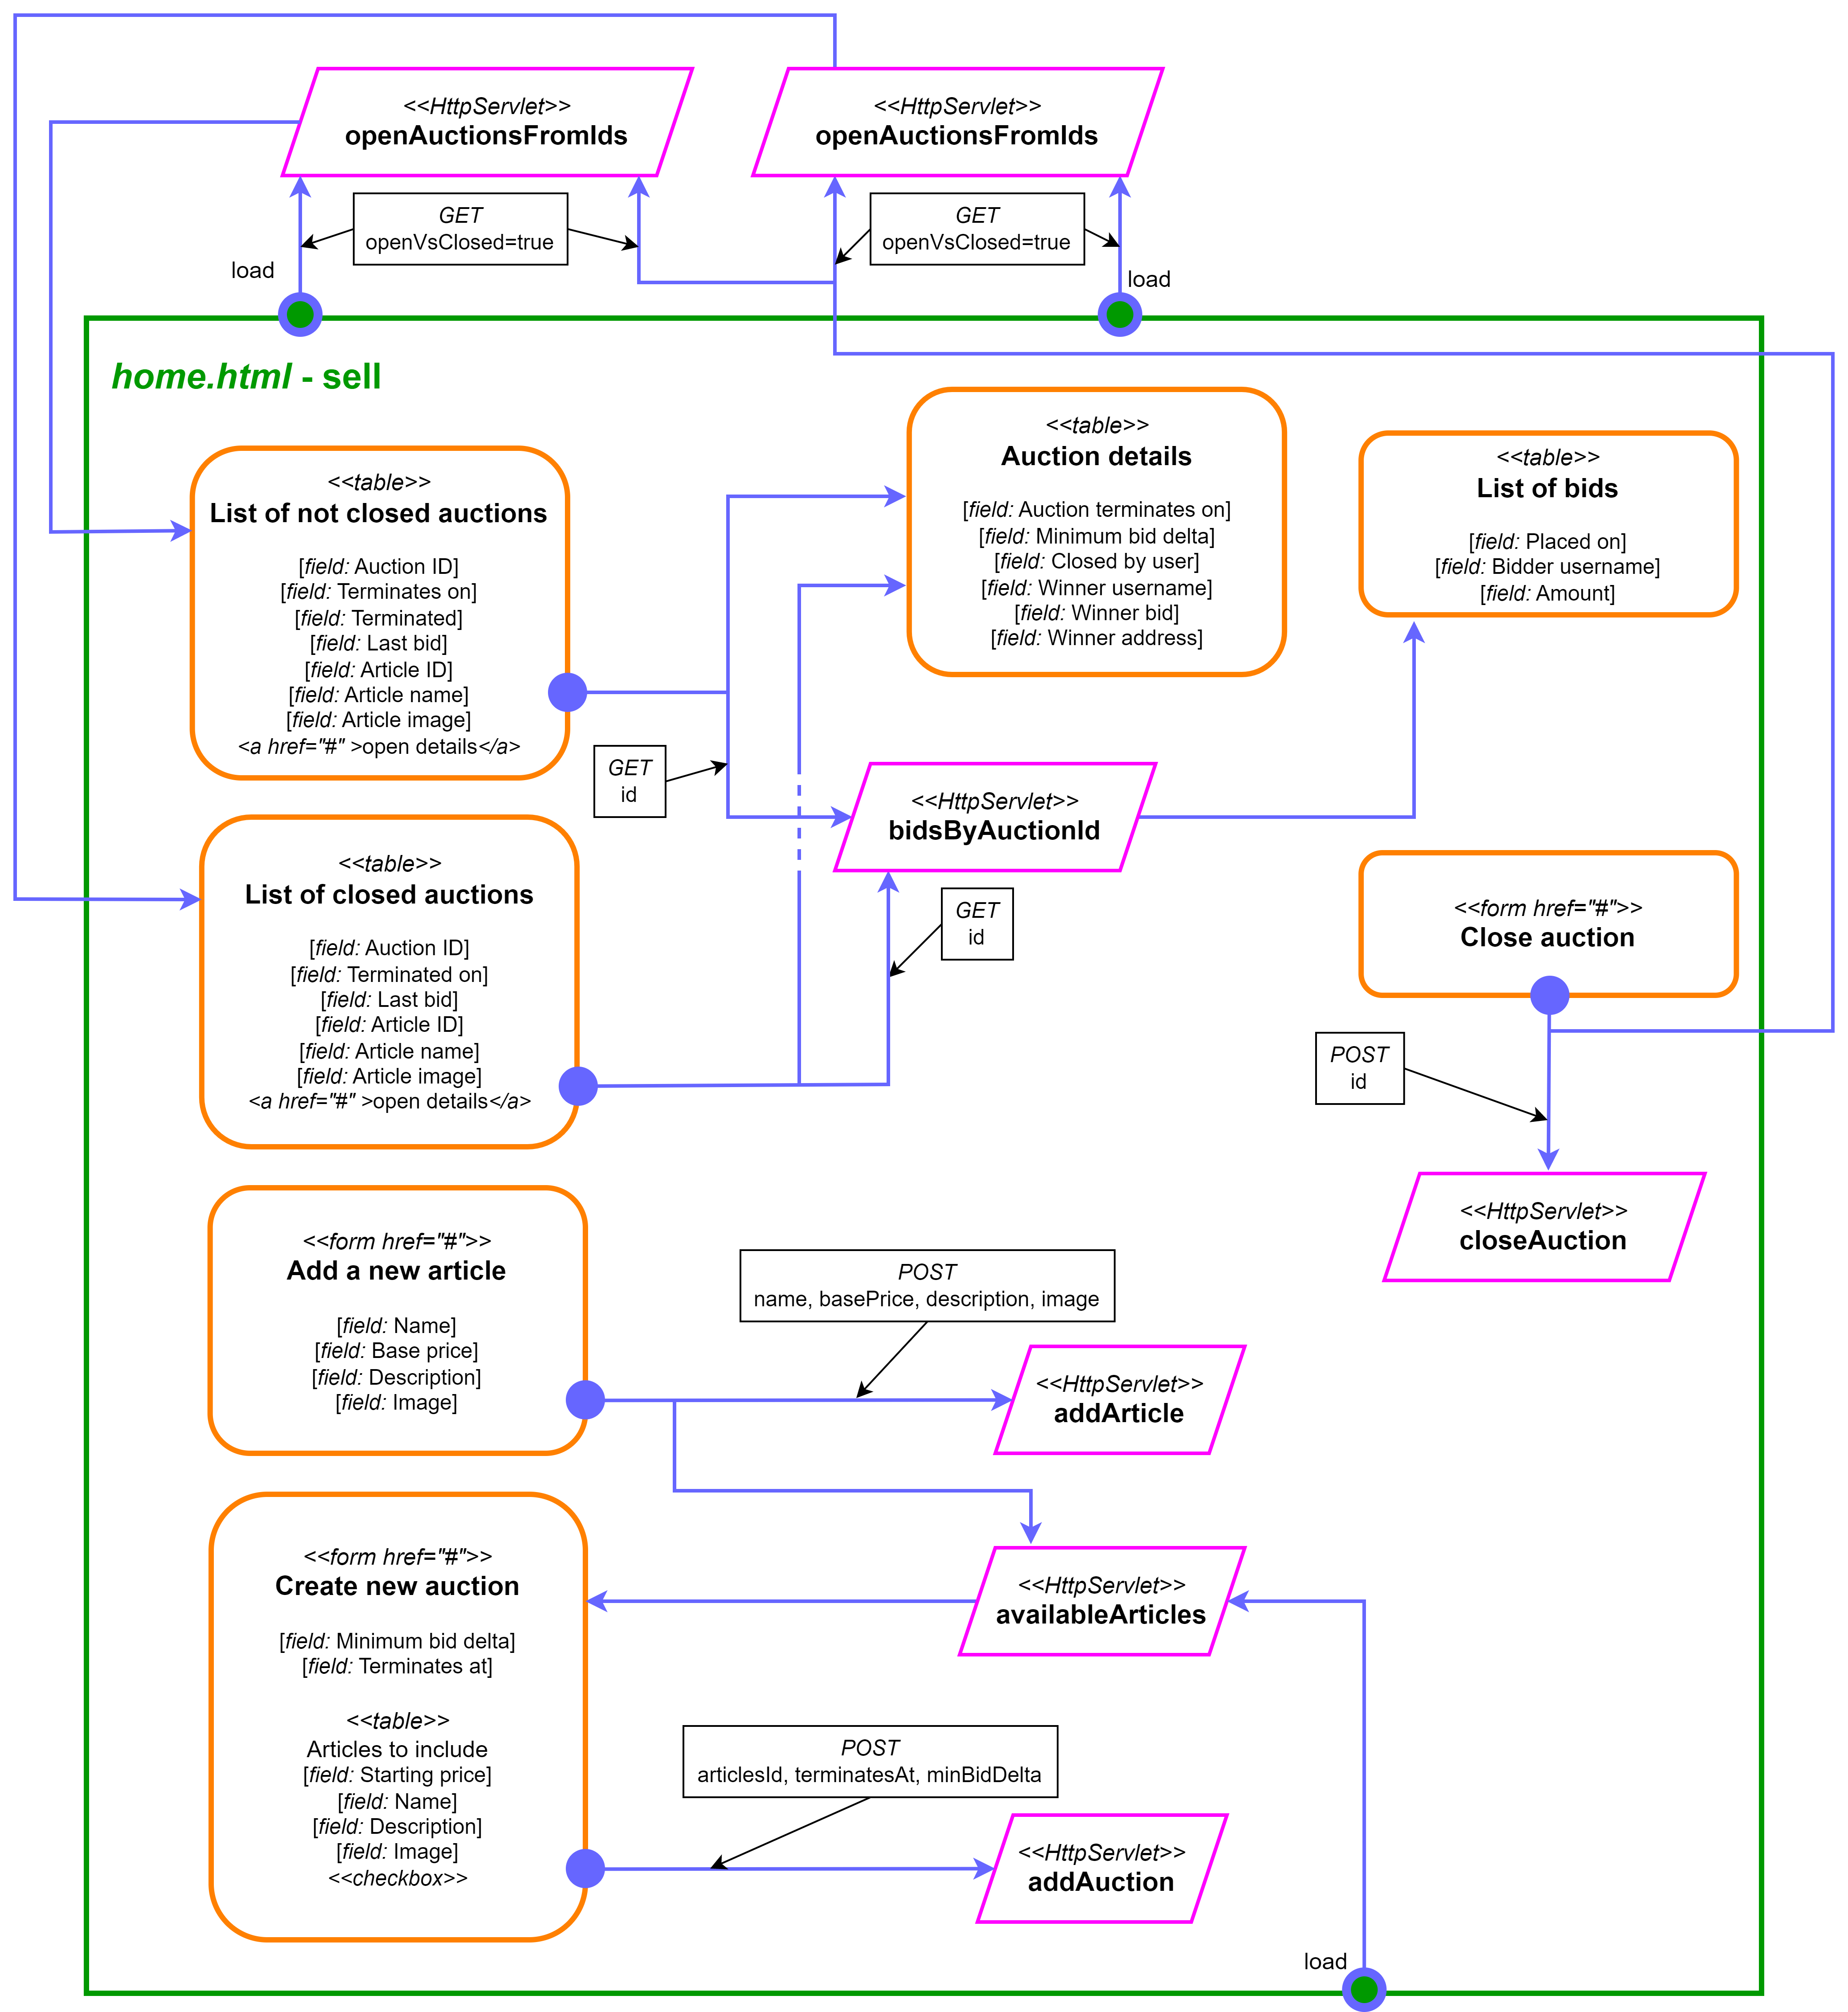
\includegraphics[width=1.2\textwidth]{RIA-design/TIWRIA-sell.png}}
				\newpage
				
			\subsection{Navigation Elements}
				The navigation menu allows the user to log out and choose between the buying and selling functionalities. This element is positioned to the side using appropriate CSS definitions.
				\begin{figure}[h]
					\noindent \makebox[\textwidth]{
						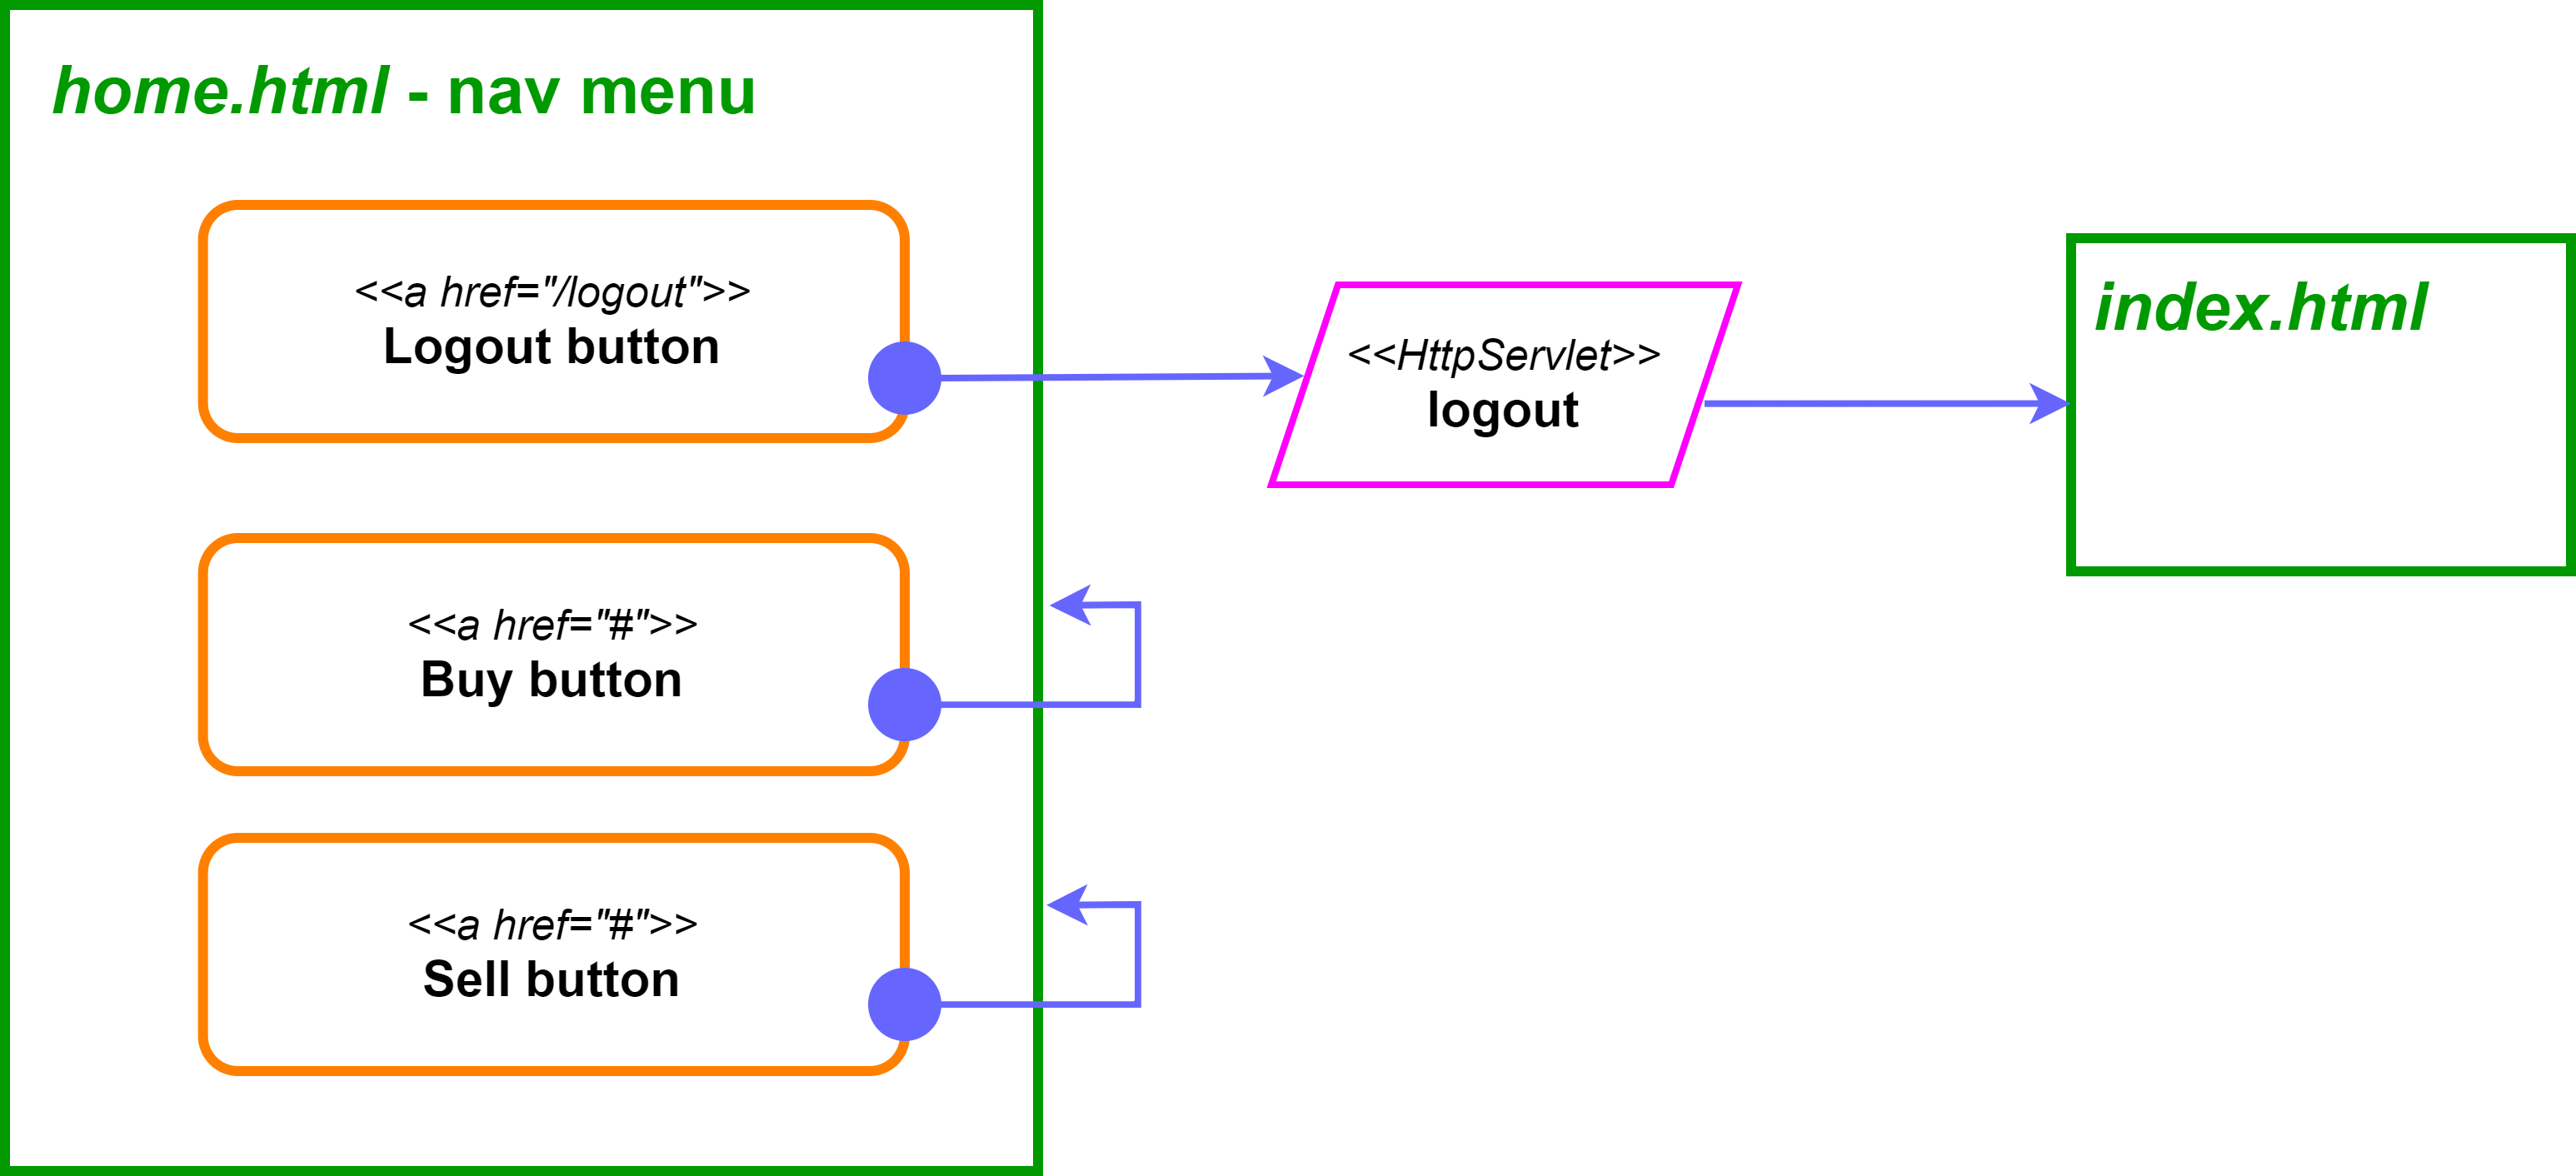
\includegraphics[width=1\textwidth]{RIA-design/TIWRIA-home.png}}
				\end{figure}
				\phantom{.}

			\subsection{Access Control and Error Handling}
				All servlets (except for `doLogin` and `logout`) require that the `user` attribute in the session contains an object of type `User`: this requirement is both practical (the data of that object is necessary) and functional (only authenticated users can use the application). To ensure this, a `loginChecker` servlet of type \textit{Filter} is used. This implements a function that returns an error code \textit{403-Forbidden} if the user is not authenticated. With this information, JavaScript utility functions for making connections check the response status and redirect the user to the login page if unauthorized.\\
				When the data sent to the server is incorrect, a \textit{status code 400} is returned. The callback functions handle this by extracting the error message from the response and displaying it to the user in the appropriate \textit{div} elements.

		\section[RIA - Events, Actions, and Controllers]{Events, Actions, and Controllers for the JavaScript Version}
			\subsection{Events and Actions}
				\begin{NiceTabular}{ | l | l || l | l | }
					\CodeBefore
					\rowcolors[gray]{3}{0.9}{1}
					\Body
					\Hline
					\Block{1-2}{Client Side} &&\Block{1-2}{Server Side} & \\
		 			Event & Action & Event & Action \\
					\Hline\Hline
					\Block{}{index.html\\> login form\\> submit} & \Block{}{Character validation\\> redirect} & \textit{POST} (user, pass) & \Block{}{Credential validation\\> load user} \\
					\Hline
					\Block{}{home.html\\> nav menu\\> click buy} & \Block{}{Load buy items} & \Block{}{\textit{GET} (ids),\\\textit{GET}} & \Block{}{Load open auctions,\\load won auctions\\with articles} \\
					\Block{}{home.html\\> nav menu\\> click sell} & \Block{}{Load sell items} & \textit{GET} & \Block{}{Load auctions\\with articles} \\
					\Block{}{home.html\\> nav menu\\> click logout} & Reset username & \textit{GET} & Close session \\
					\Hline
					\Block{}{home.html buy\\> search form\\> submit} & \Block{}{Update open auctions} & \textit{GET} (query)& \Block{}{Load auctions\\with search} \\
					\Block{}{home.html buy\\> open auctions list\\> click open details} & \Block{}{Update detail} & \textit{GET} (id) & \Block{}{Load articles,\\load bids} \\
					\Block{}{home.html buy\\> won auctions list\\> click open details} & \Block{}{Update detail} & \textit{GET} (id) & \Block{}{Load articles,\\load bids} \\
					\Block{}{home.html buy\\> auction detail\\> submit bid} & Update bids & \Block{}{\textit{POST} (auction,\\bid),\\\textit{GET}} & \Block{}{Update bids\\> load bids} \\
					\Hline					
					\Block{}{home.html sell\\> non-closed auctions list\\> click open details} & \Block{}{Update detail\\with close form} & \textit{GET} (id) & \Block{}{Load bids} \\
					\Block{}{home.html sell\\> closed auctions list\\> click open details} & \Block{}{Update detail} & \textit{GET} (id) & \Block{}{Load bids} \\
					\Block{}{home.html sell\\> add article form\\> submit} & \Block{}{Update available articles list} & \Block{}{\textit{POST}\\(name, desc,\\price, image)} & \Block{}{Add article\\> load available \\articles} \\
					\Block{}{home.html sell\\> create auction form\\> submit} & \Block{}{Update available articles,\\update non-closed auctions} & \Block{}{\textit{POST} (raise,\\date, article list),\\\textit{GET},\\\textit{GET}} & \Block{}{Create auction\\> load articles,\\load closed and \\non-closed auctions} \\
					\Block{}{home.html sell\\> close auction form\\> submit} & Update auctions & \Block{}{\textit{POST} (id),\\\textit{GET},\\\textit{GET}} & \Block{}{Close auction\\> load closed and \\non-closed auctions} \\
					\Hline
				\end{NiceTabular}
				\newpage
				
			\subsection{Events and Controllers}
				\begin{NiceTabular}{ | l | l || l | l | }
					\CodeBefore
					\rowcolors[gray]{3}{0.9}{1}
					\Body
					\Hline
					\Block[c]{1-2}{Client Side} &&\Block{1-2}{Server Side} & \\
					Event & Controller & Event & Controller \\
					\Hline\Hline
					\Block{}{index.html\\> login form\\> submit} & \Block{}{handleEvent\\> makeCall\\> update} & \textit{POST} (user, pass) & doLogin \\
					\Hline
					\Block{}{home.html\\> nav menu\\> click buy} & \Block{}{loadBuy\\> makeCall\\> initBuy} & \Block{}{\textit{GET} (ids),\\\textit{GET}} & \Block{}{auctionsFromIds,\\wonAuctionsWithArticles} \\
					\Block{}{home.html\\> nav menu\\> click sell} & \Block{}{loadSell\\> makeCall\\> initSell} & \textit{GET} & \Block{}{auctionsForOwner,\\availableArticles} \\
					\Block{}{home.html\\> nav menu\\> click logout} & logout & \textit{GET} & logout \\
					\Hline
					\Block{}{home.html buy\\> search form\\> submit} & \Block{}{show\\> makeCall\\> update} & \textit{GET} (query)& openAuctionsWithSearch \\
					\Block{}{home.html buy\\> open auctions list\\> click open details} & \Block{}{show\\> makeCall\\> update} & \textit{GET} (id) & \Block{}{articlesByAuctionId,\\bidsByAuctionId} \\
					\Block{}{home.html buy\\> won auctions list\\> click open details} & \Block{}{show\\> makeCall\\> update} & \textit{GET} (id) & \Block{}{articlesByAuctionId,\\bidsByAuctionId} \\
					\Block{}{home.html buy\\> auction detail\\> submit bid} & \Block{}{handleBidPlacement\\> makeCall\\> bidsRefreshCallBack} & \Block{}{\textit{POST} (auction,\\bid),\\\textit{GET}} & \Block{}{placeBid\\> bidsByAuctionId}\\
					\Hline					
					\Block{}{home.html sell\\> non-closed auctions list\\> click open details} & \Block{}{show\\> makeCall\\> update} & \textit{GET} (id) & \Block{}{bidsByAuctionId} \\
					\Block{}{home.html sell\\> closed auctions list\\> click open details} & \Block{}{show\\> makeCall\\> update} & \textit{GET} (id) & \Block{}{bidsByAuctionId} \\
					\Block{}{home.html sell\\> add article form\\> submit} & \Block{}{handleEvent\\> makeCall\\> articlesRefresh} & \Block{}{\textit{POST}\\(name, desc,\\price, image)} & \Block{}{addArticle\\> availableArticles} \\
					\Block{}{home.html sell\\> create auction form\\> submit} & \Block{}{handleEvent\\> makeCall\\> show} & \Block{}{\textit{POST} (raise,\\date, article list),\\\textit{GET},\\\textit{GET}} & \Block{}{addAuction\\> availableArticles,\\auctionsForOwner} \\
					\Block{}{home.html sell\\> close auction form\\> submit} & \Block{}{handleAuctionClosing\\> makeCall\\> auctionClosedUpdate} & \Block{}{\textit{POST} (id),\\\textit{GET},\\\textit{GET}} & \Block{}{closeAuction\\> auctionsForOwner} \\
					\Hline
				\end{NiceTabular}
				\newpage
		\section[RIA - Components]{Components for the JavaScript Version}
			\subsection{Database Access, Data Beans, and DAOs}
				For the components related to \hyperref[accessodb]{database access}, \hyperref[databeans]{data beans}, and \hyperref[dao]{DAO functionality}, please refer to the section dedicated to the HTML-only version, as these remain unchanged.

			\subsection{Servlets}
				\subsubsection{Controllers}
					\begin{itemize}
						\item doLogin
						\item auctionsFromIds
						\item openAuctionsWithSearch
						\item wonAuctionsWithArticles
						\item articlesByAuctionId
						\item bidsByAuctionId
						\item placeBid
						\item auctionsForOwner
						\item availableArticles
						\item addArticle
						\item addAuction
						\item closeAuction
						\item logout
					\end{itemize}
				\subsubsection{Filters}
					\begin{itemize}
						\item loginChecker
					\end{itemize}

			\subsection{Client-Side Views}
				The components that manage a specific view generally consist of the following methods:
				\begin{itemize}
					\item \textbf{init}, used during page load;
					\item \textbf{show} and \textbf{handleEvent}, registered as event handlers, invoke \texttt{makeCall};
					\item \textbf{callback}, invoked by \texttt{makeCall} when the server responds with the requested data, calls \texttt{update} when no errors occur;
					\item \textbf{update}, used to update the HTML page through the DOM.
				\end{itemize}
				\phantom{.}\\
				The client-side JavaScript code is structured as follows:

				\subsubsection{utils.js}
					Utility functions common to multiple components of the application:
					\begin{itemize}
						\item \textbf{logout};
						\item various \textbf{makeCall} functions, depending on how the parameters should be passed to the server;
						\item \textbf{autoClicker}, a utility object with the \texttt{autoClick} method to click the first anchor in the provided DOM object;
						\item utility functions for working with \textbf{dates} and properly formatting a timestamp;
						\item \textbf{auctionDetailsShow} and \textbf{auctionWithArticlesCallback}, common functions for multiple components;
						\item functions to save auction data in the session \textbf{storage} and retrieve that information;
						\item \textbf{setLastAction}, to store the last performed action in permanent local storage;
						\item \textbf{BidsList}, a component that manages a list of bids for a given auction.
					\end{itemize}

				\subsubsection{home.js}
					\textit{PageOrchestrator}, responsible for loading the buy/sell functionalities and constructing the objects that interact with the DOM. Key methods of this component include:
					\begin{itemize}
						\item init: retrieves the username, initializes event listeners in the navigation menu, fetches the last action, and determines whether to load the buy or sell functionalities;
						\item initBuy: constructs all the components for the buy functionality and initializes them, registering event listeners;
						\item initSell: constructs all the components for the sell functionality and initializes them, registering event listeners.
					\end{itemize}
				\phantom{.}\\
				Each component of the buy and sell functionalities is associated with a constructor, so that all the necessary functions for that component become methods of the object that will be created. Here are the constructors for each:

				\subsubsection{buy.js}
					\begin{itemize}
						\item \textbf{saveAuctionAsVisited}, a utility function;
						\item \textbf{OpenAuctionsWithSearch}, a table to search through open auctions;
						\item \textbf{ArticlesList}, a list of articles in the details of an auction;
						\item \textbf{AuctionDetails}, the outermost div of auction details, contains the form to place a bid;
						\item \textbf{WonAuctionsWithArticles}, a table of won auctions and the associated articles.
					\end{itemize}

				\subsubsection{sell.js}
					\begin{itemize}
						\item \textbf{AuctionsWithArticles}, a list of auctions with their articles, used for both open and closed auctions;
						\item \textbf{AuctionDetailsOwner}, the outermost div of auction details, optionally contains the button to close the auction;
						\item \textbf{AddArticle}, a form for adding a new article;
						\item \textbf{AddAuction}, a form for creating an auction, includes the list of available articles.
					\end{itemize}
		\section[RIA - Events and Sequence Diagrams]{Events and Sequence Diagrams for the JavaScript Version}
			\subsubsection{A user logs in}
				\phantom{.}\\
				\noindent \makebox[\textwidth]{
					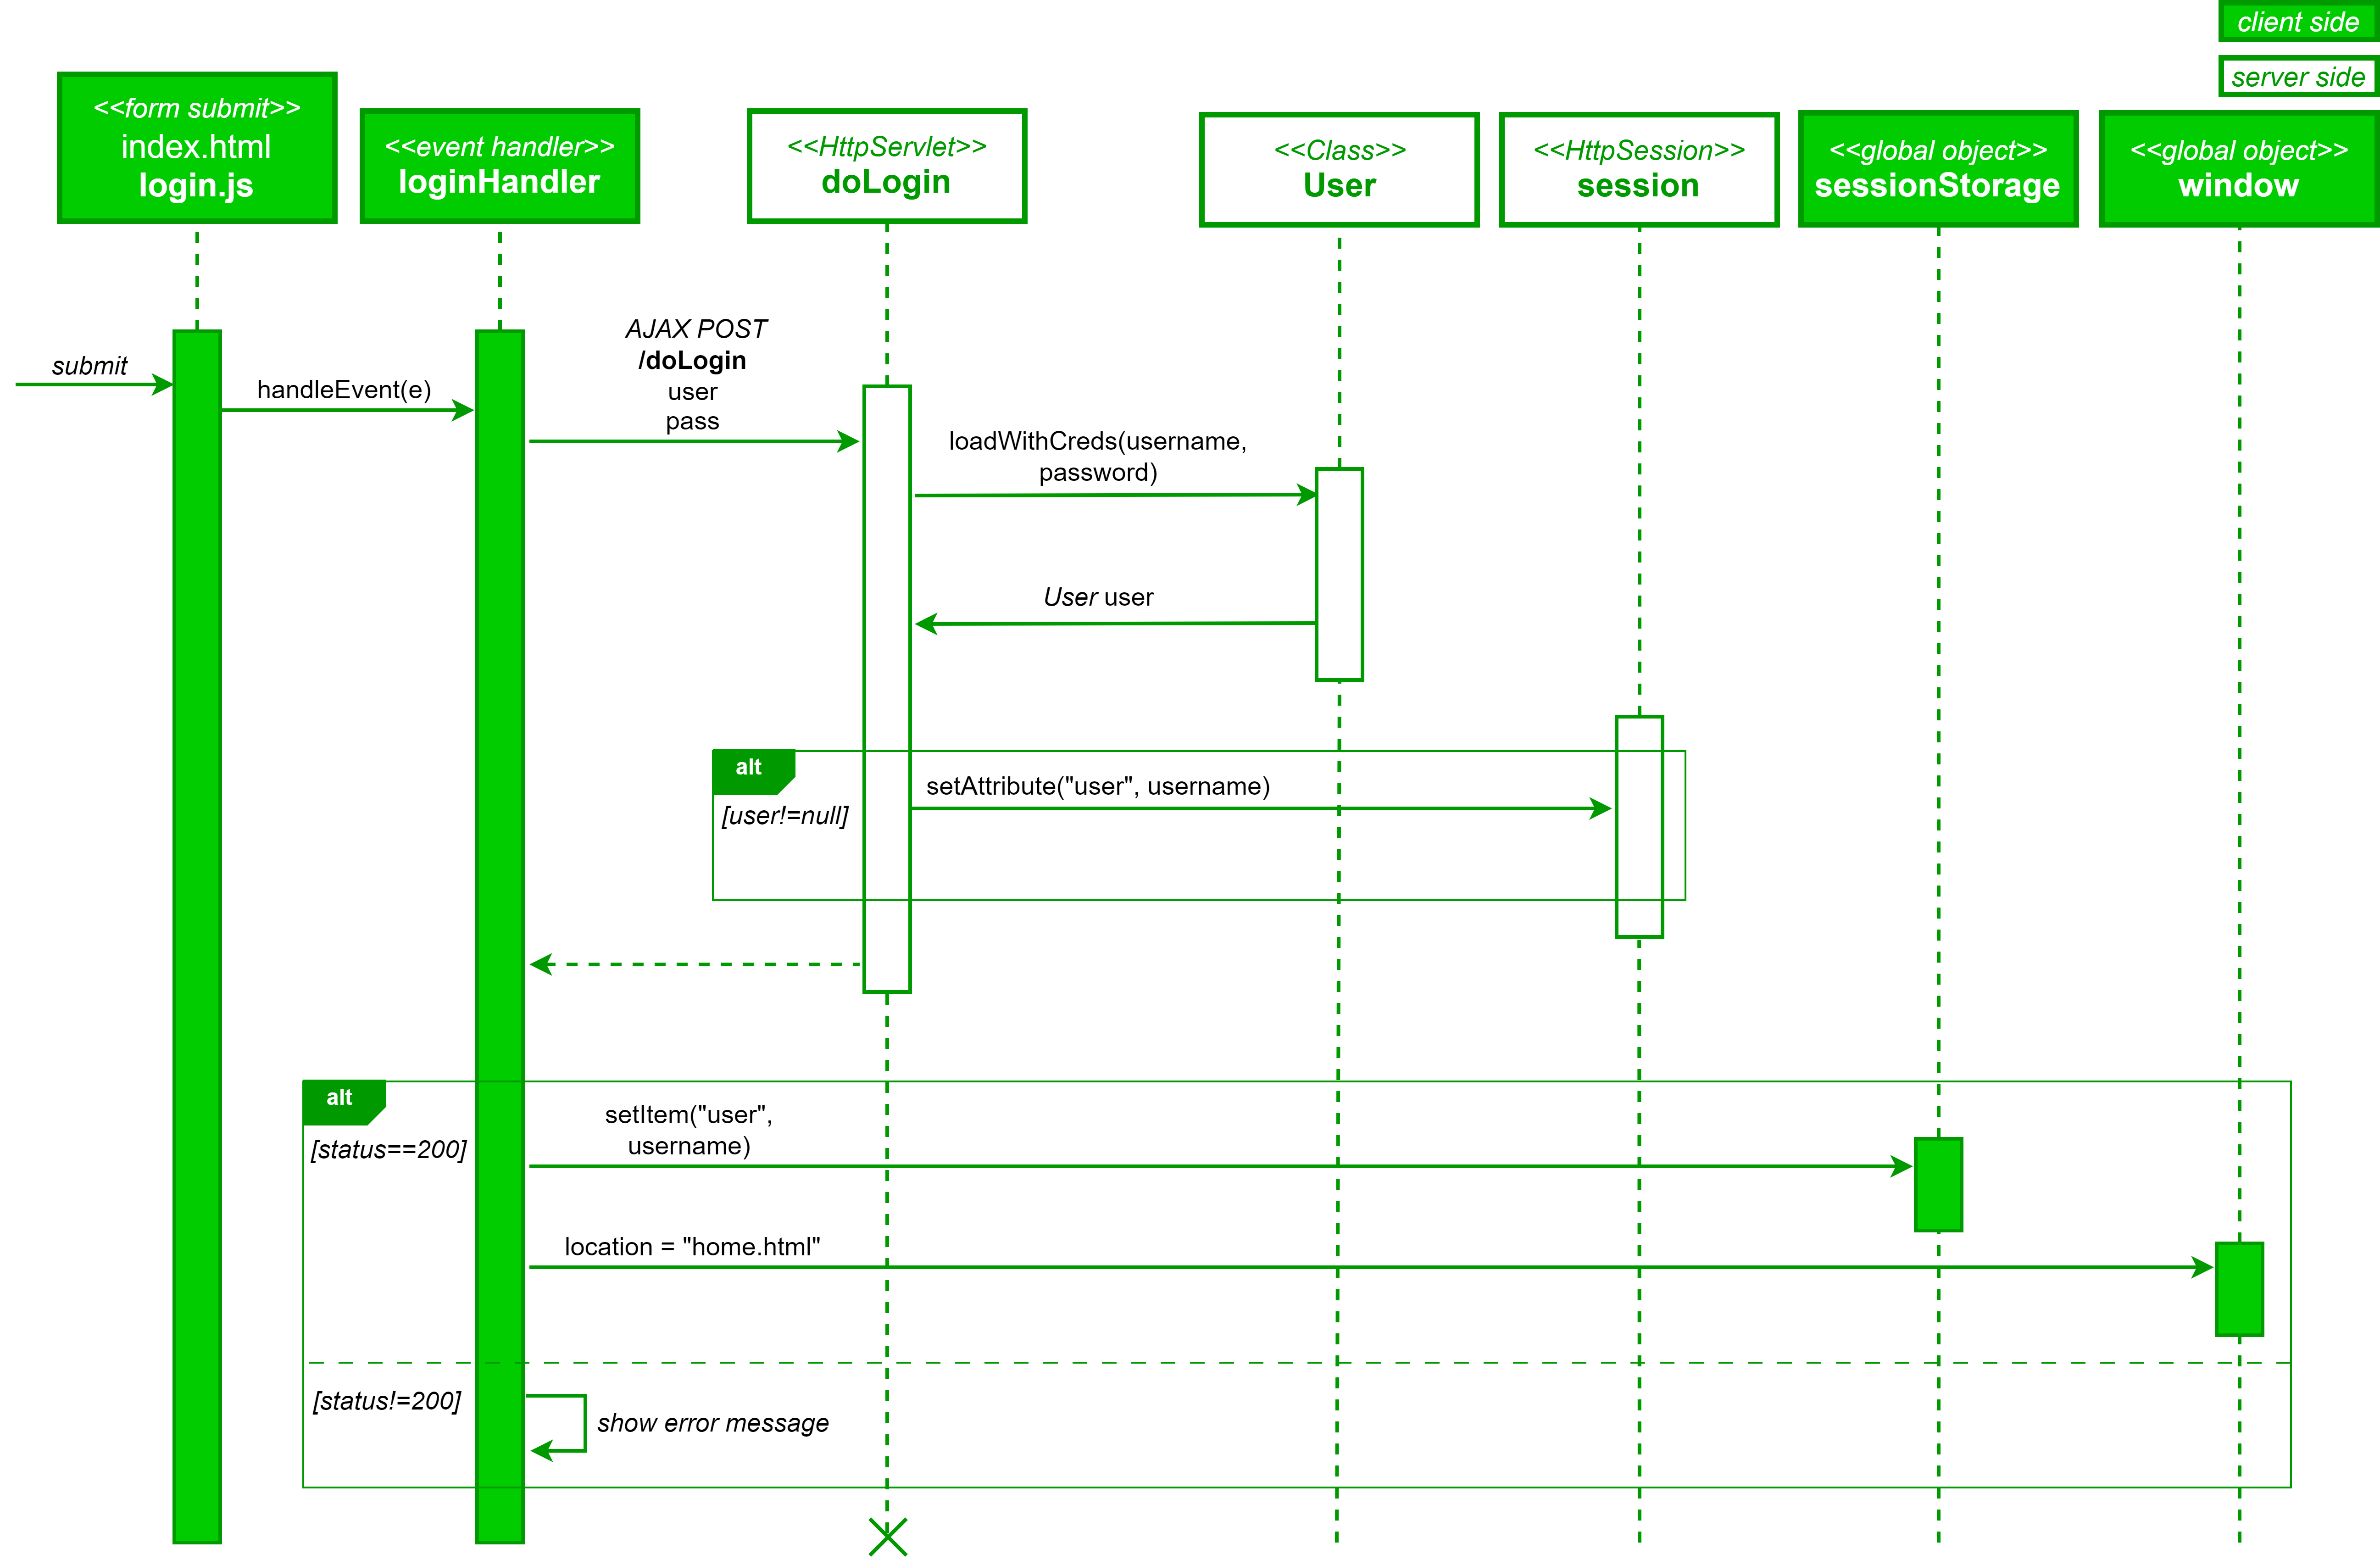
\includegraphics[width=1.25\textwidth]{RIA-SequenceDiagrams/TIWRIA-login.png}}
				\phantom{.}\\
				\newpage
			
			\subsubsection{The user requests the BUY functionality}
				\phantom{.}\\
				\noindent \makebox[\textwidth]{
					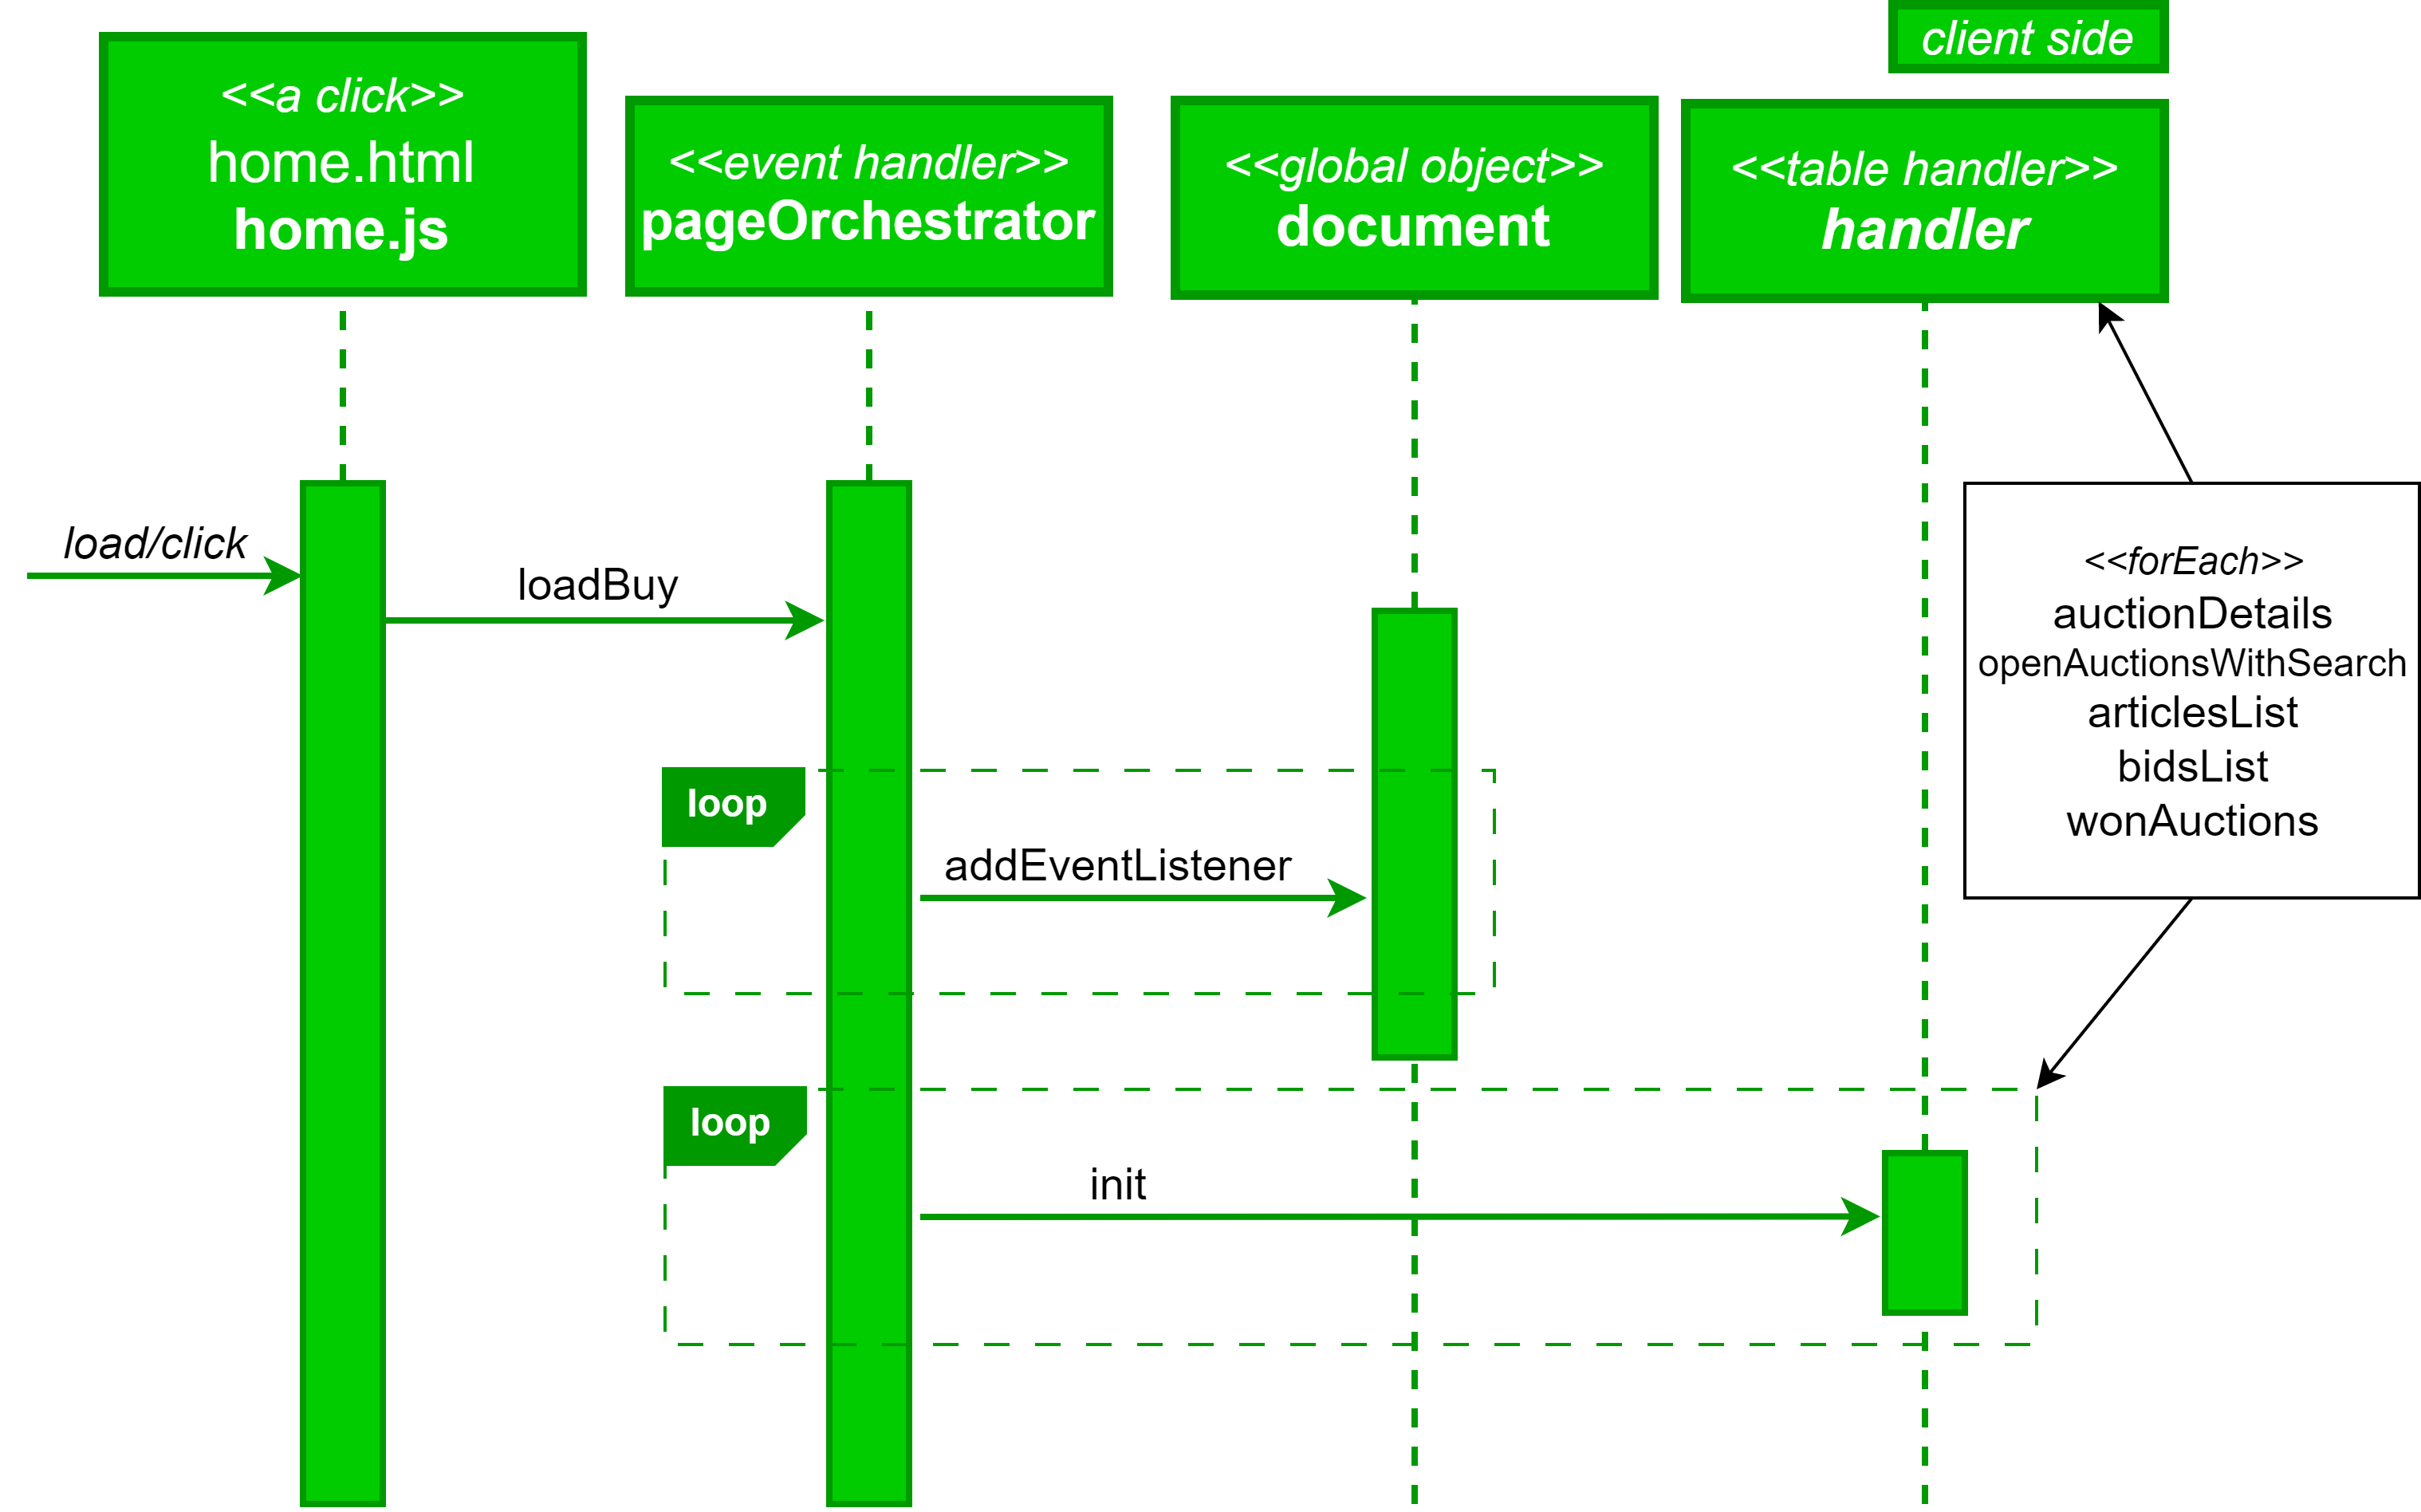
\includegraphics[width=0.85\textwidth]{RIA-SequenceDiagrams/TIWRIA-loadBuy.png}}			
				\phantom{.}\\
				\noindent \makebox[\textwidth]{
					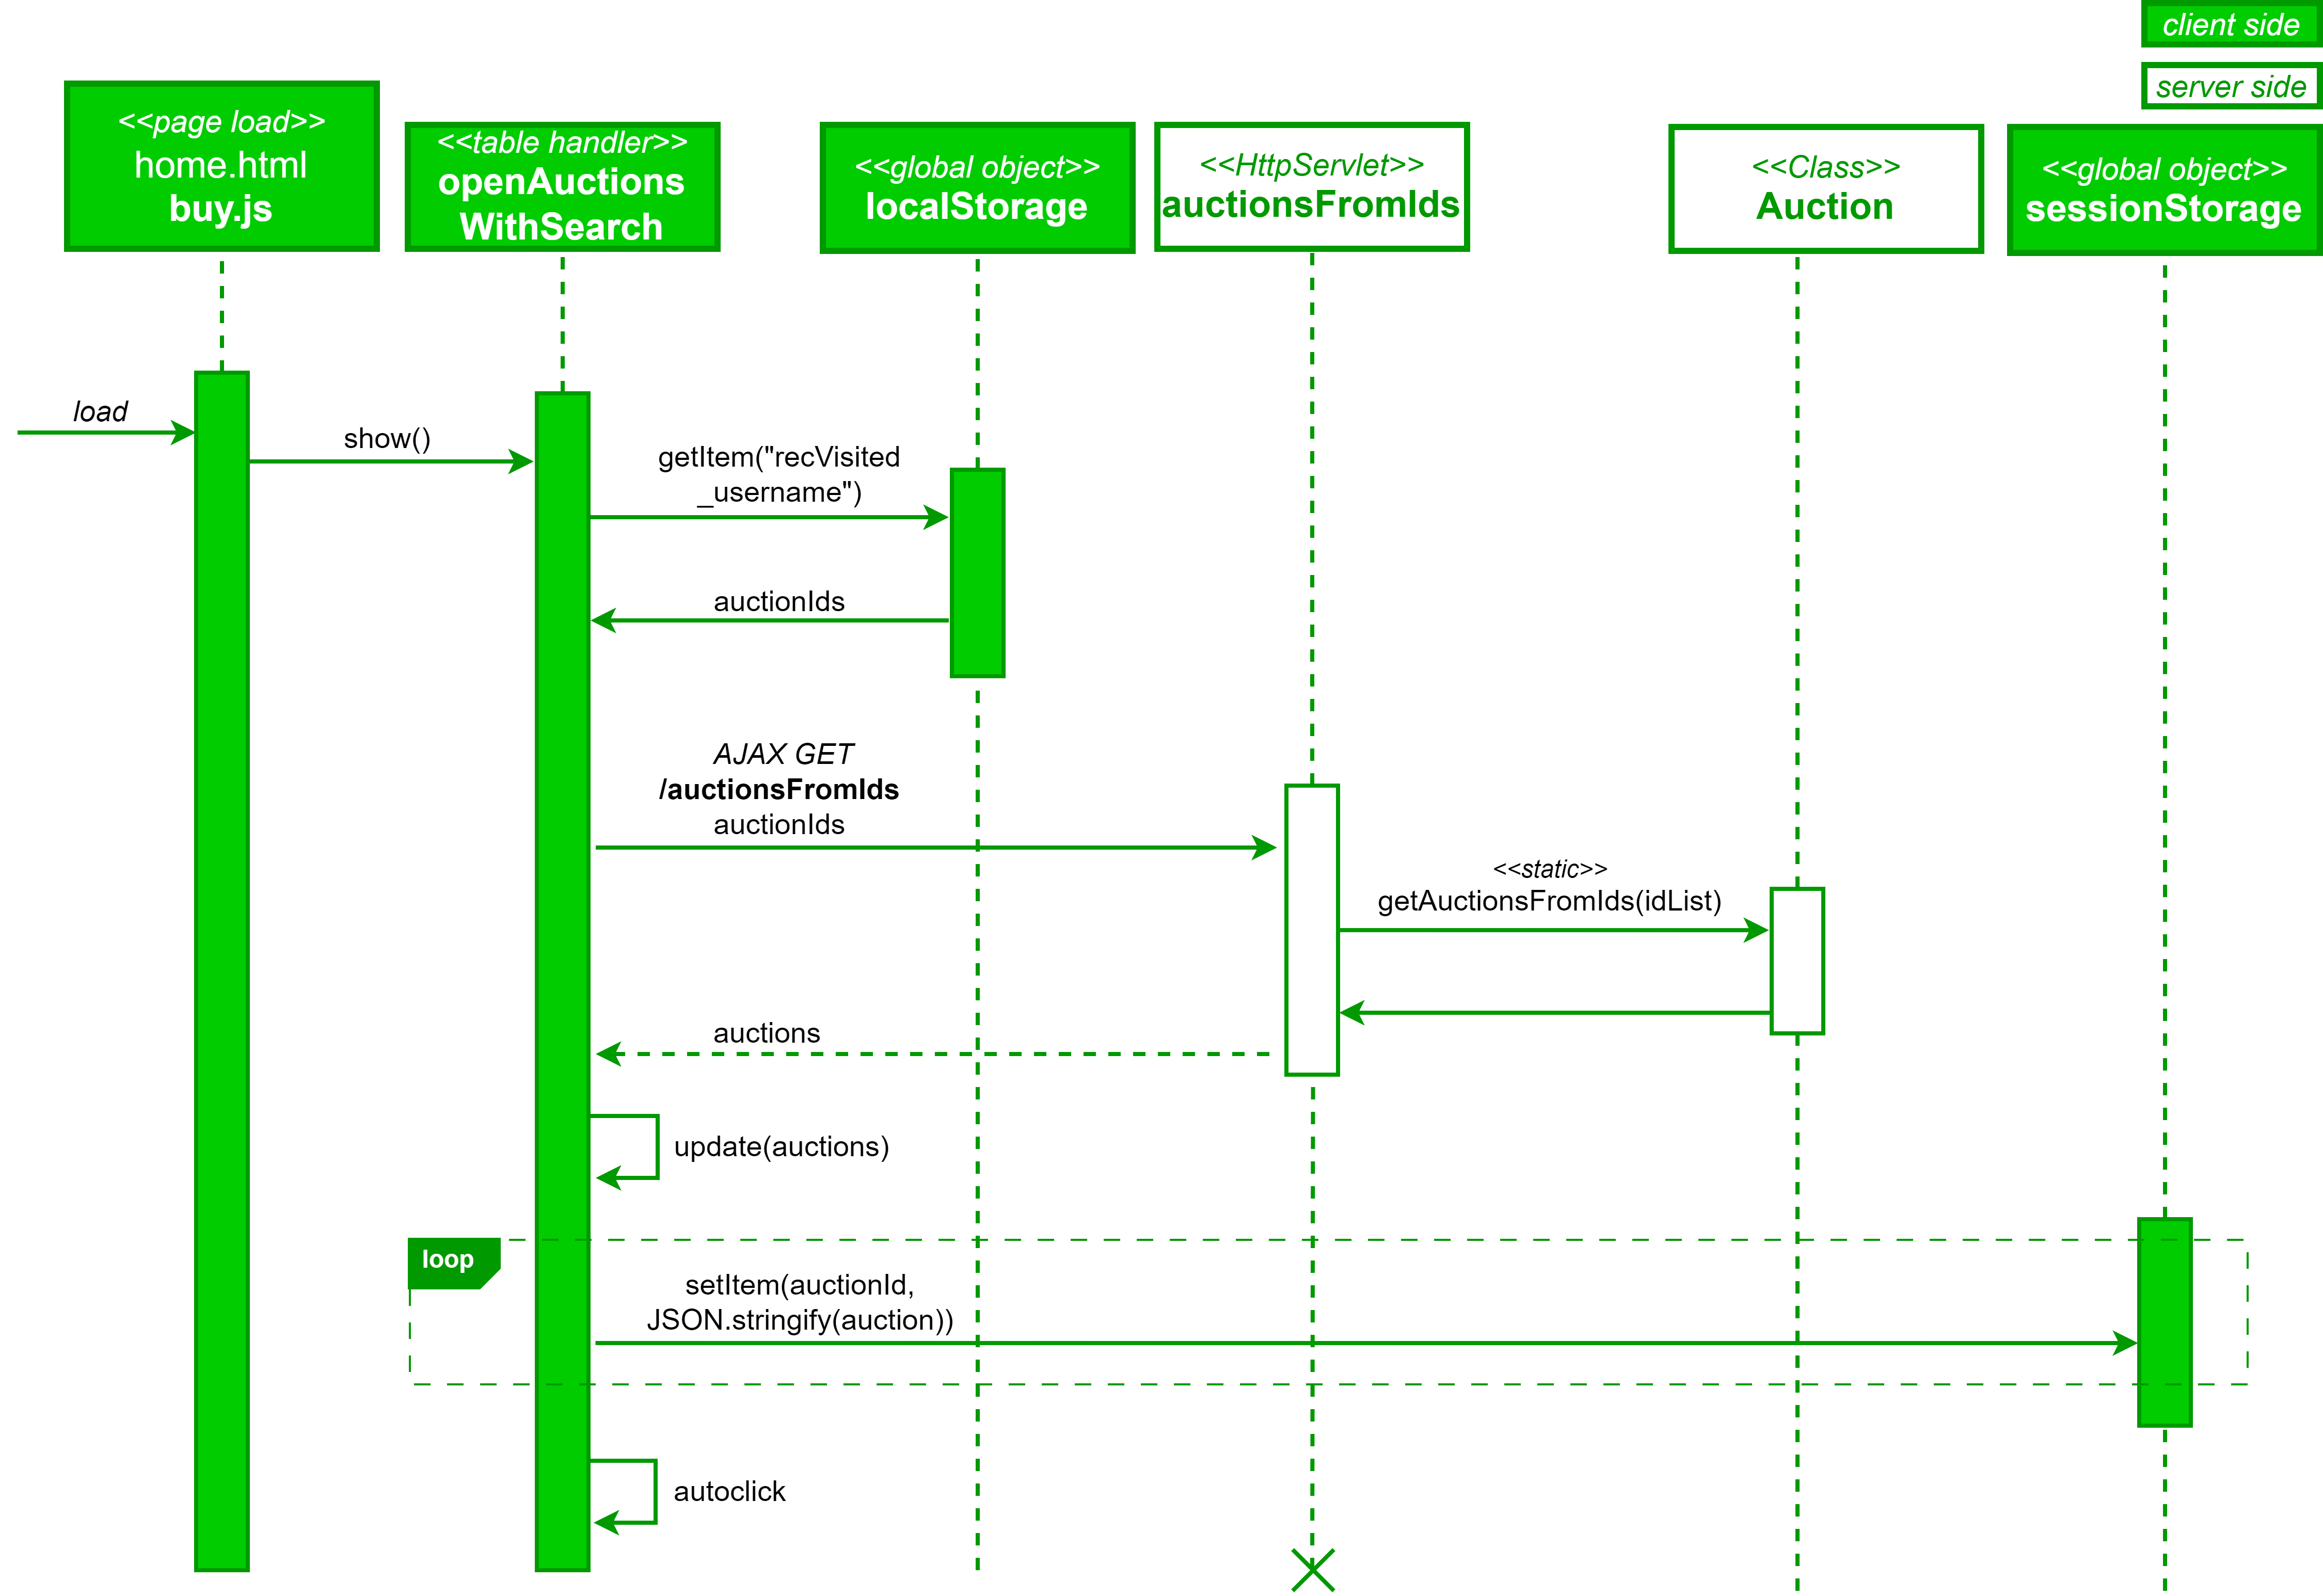
\includegraphics[width=1\textwidth]{RIA-SequenceDiagrams/TIWRIA-loadAuctionsWithSearch.png}}
				\newpage
				\phantom{.}\\
				\noindent \makebox[\textwidth]{
					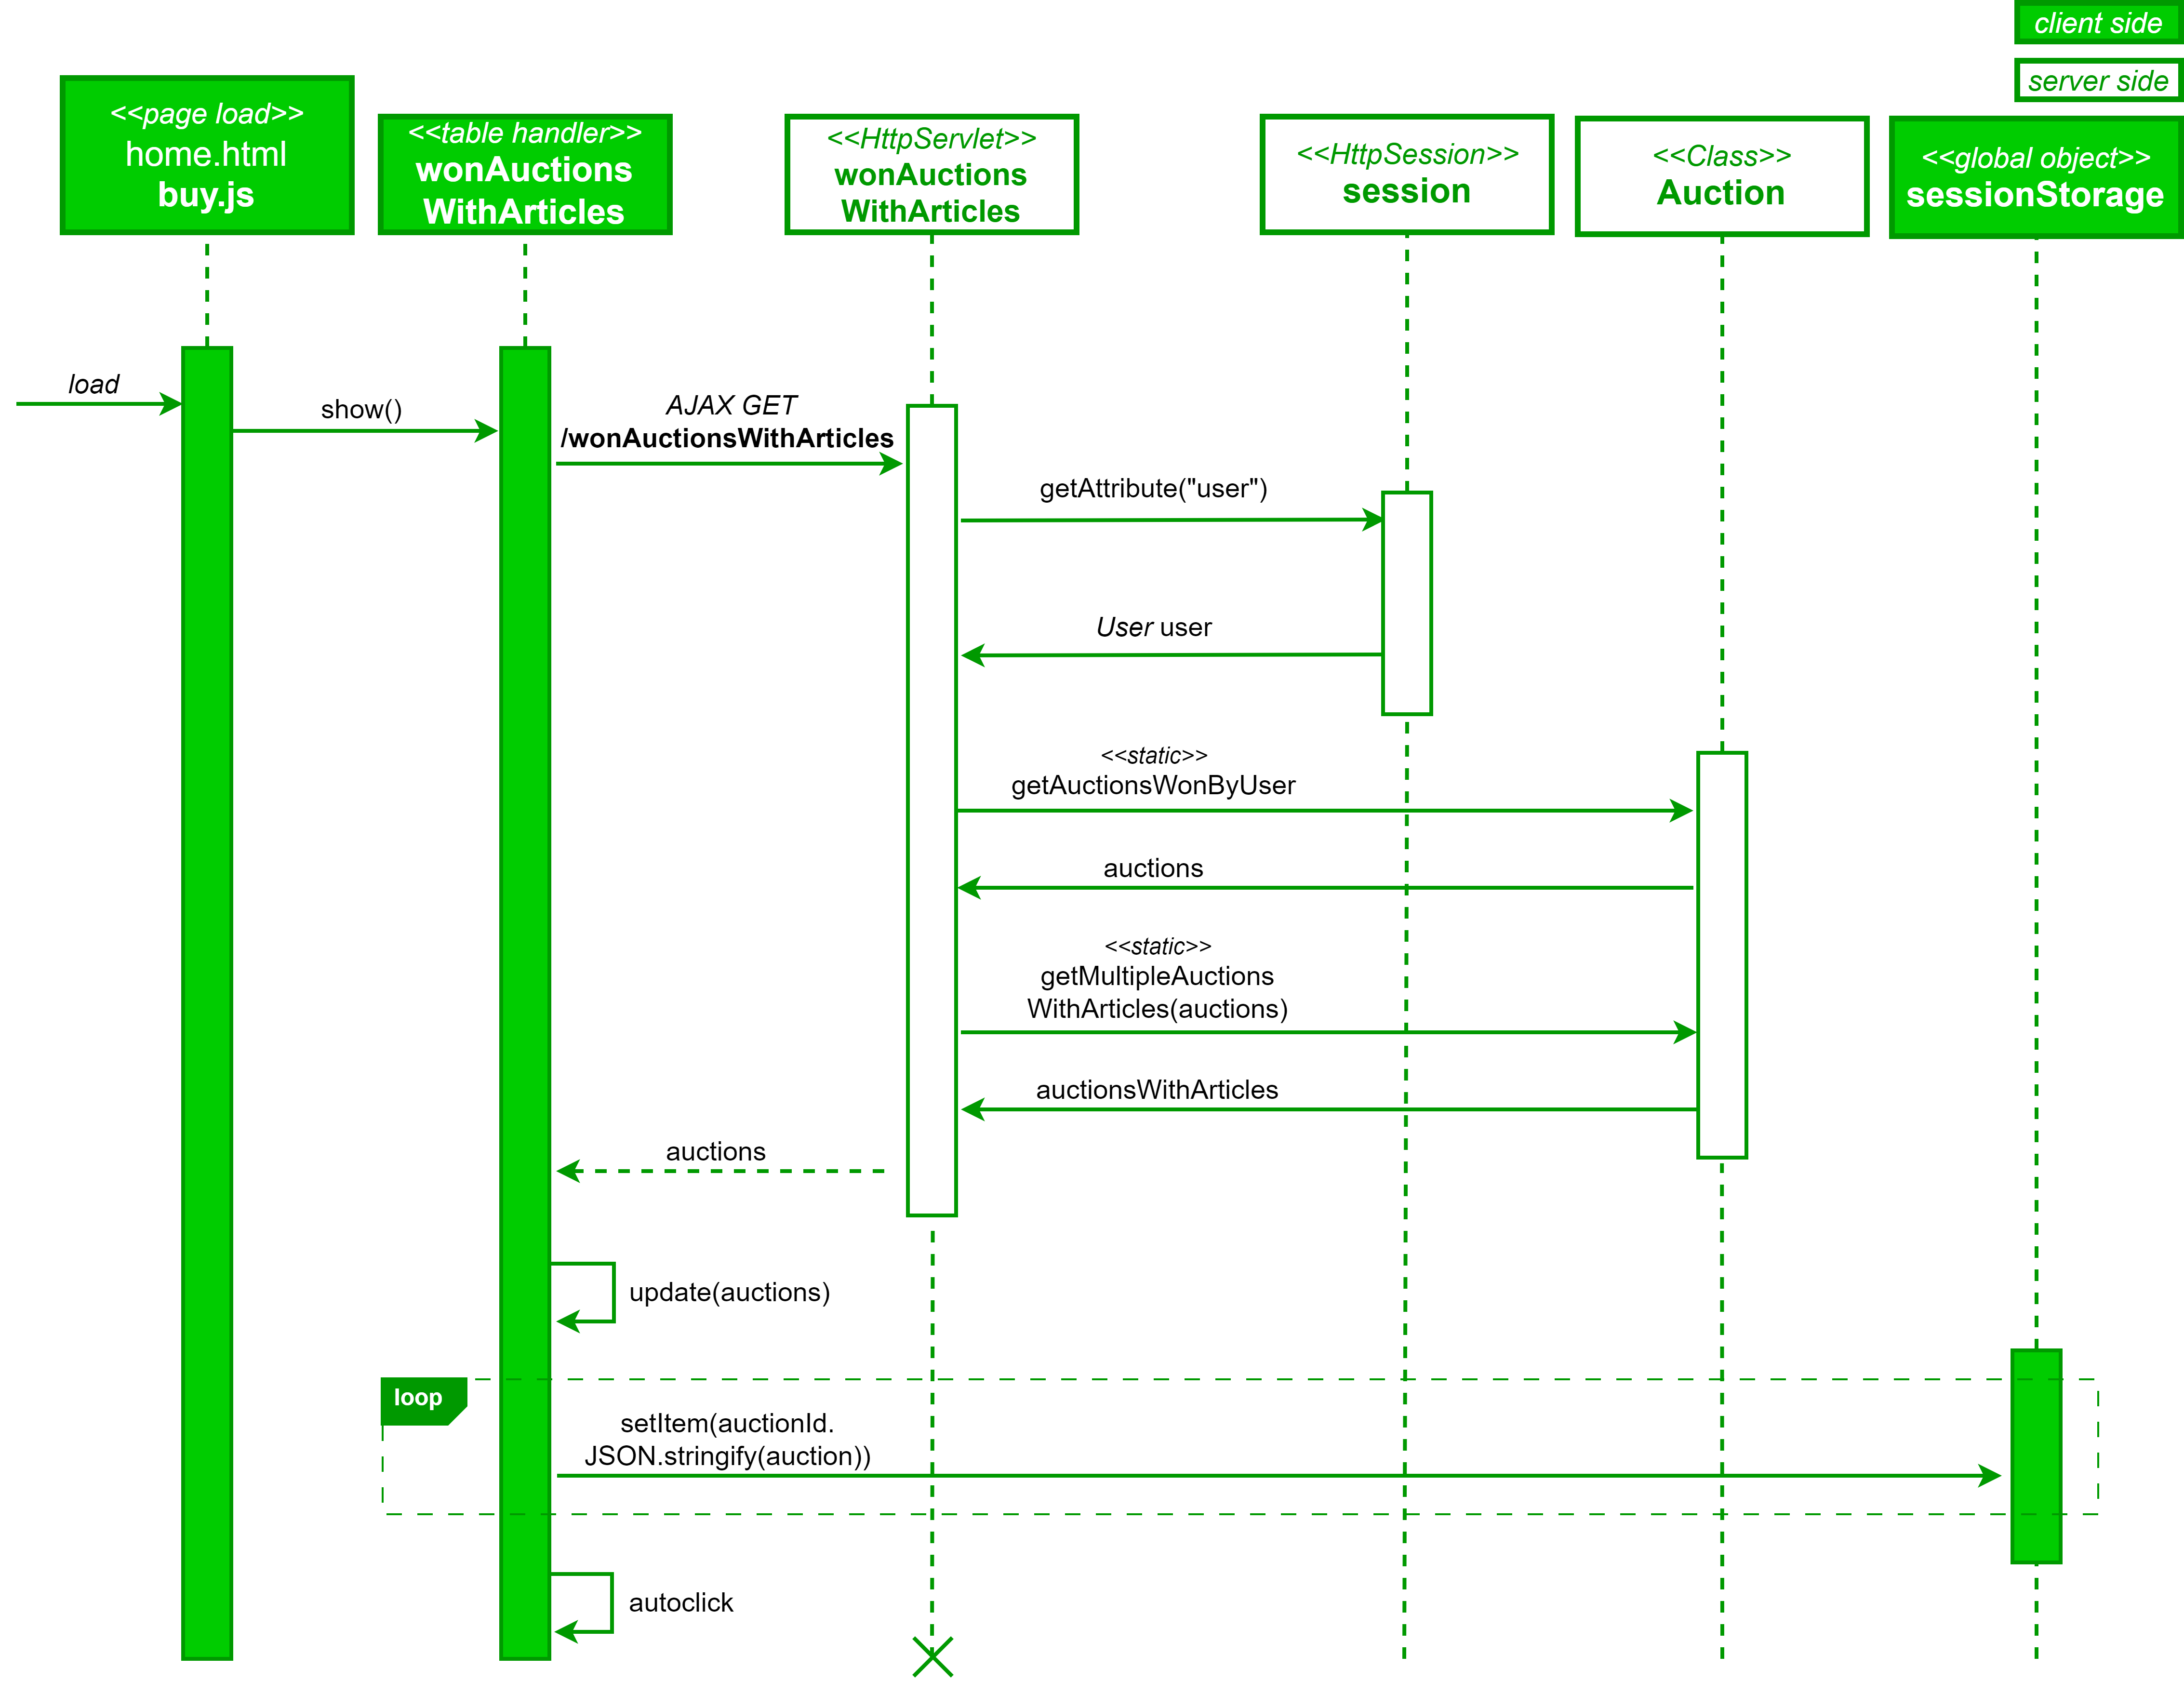
\includegraphics[width=1.1\textwidth]{RIA-SequenceDiagrams/TIWRIA-loadWonAuctions.png}}
			\subsubsection{The user enters a query to search among the auctions}
				\phantom{.}\\
				\noindent \makebox[\textwidth]{
					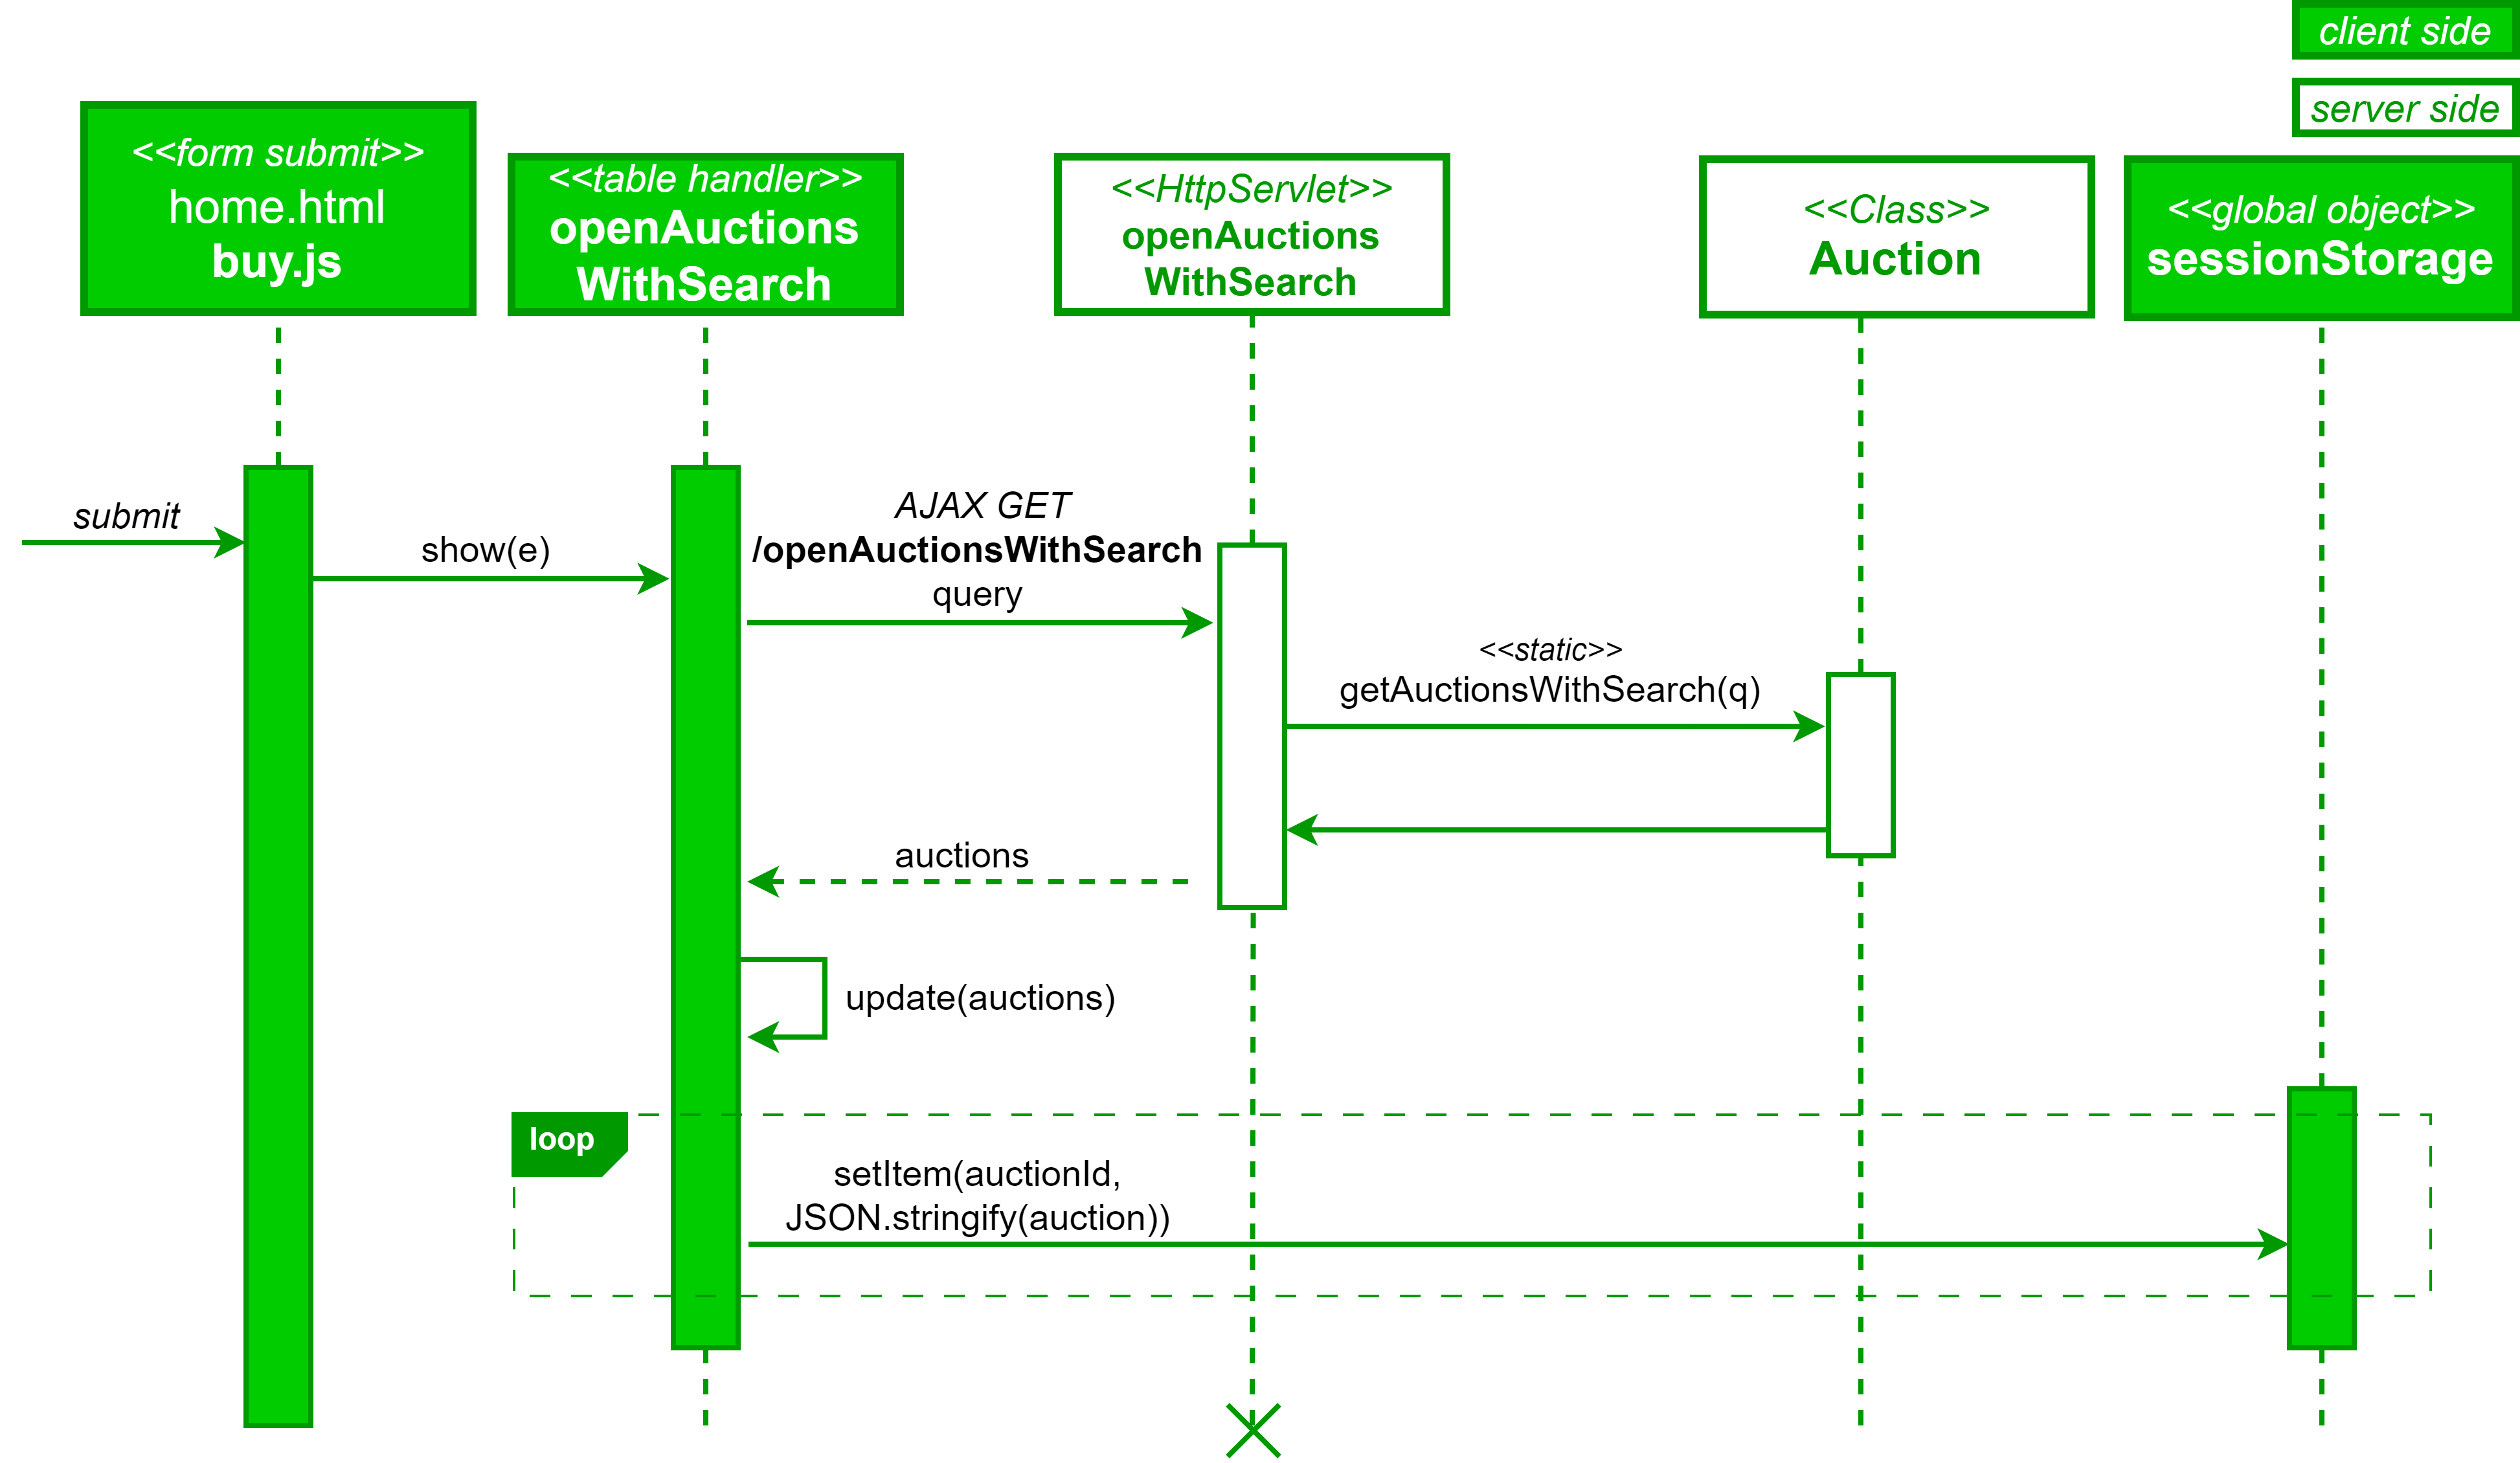
\includegraphics[width=1\textwidth]{RIA-SequenceDiagrams/TIWRIA-searchAuction.png}}				
				\newpage
			
			\subsubsection{The user clicks to view the details of an auction}
				\phantom{.}\\
				\noindent \makebox[\textwidth]{
					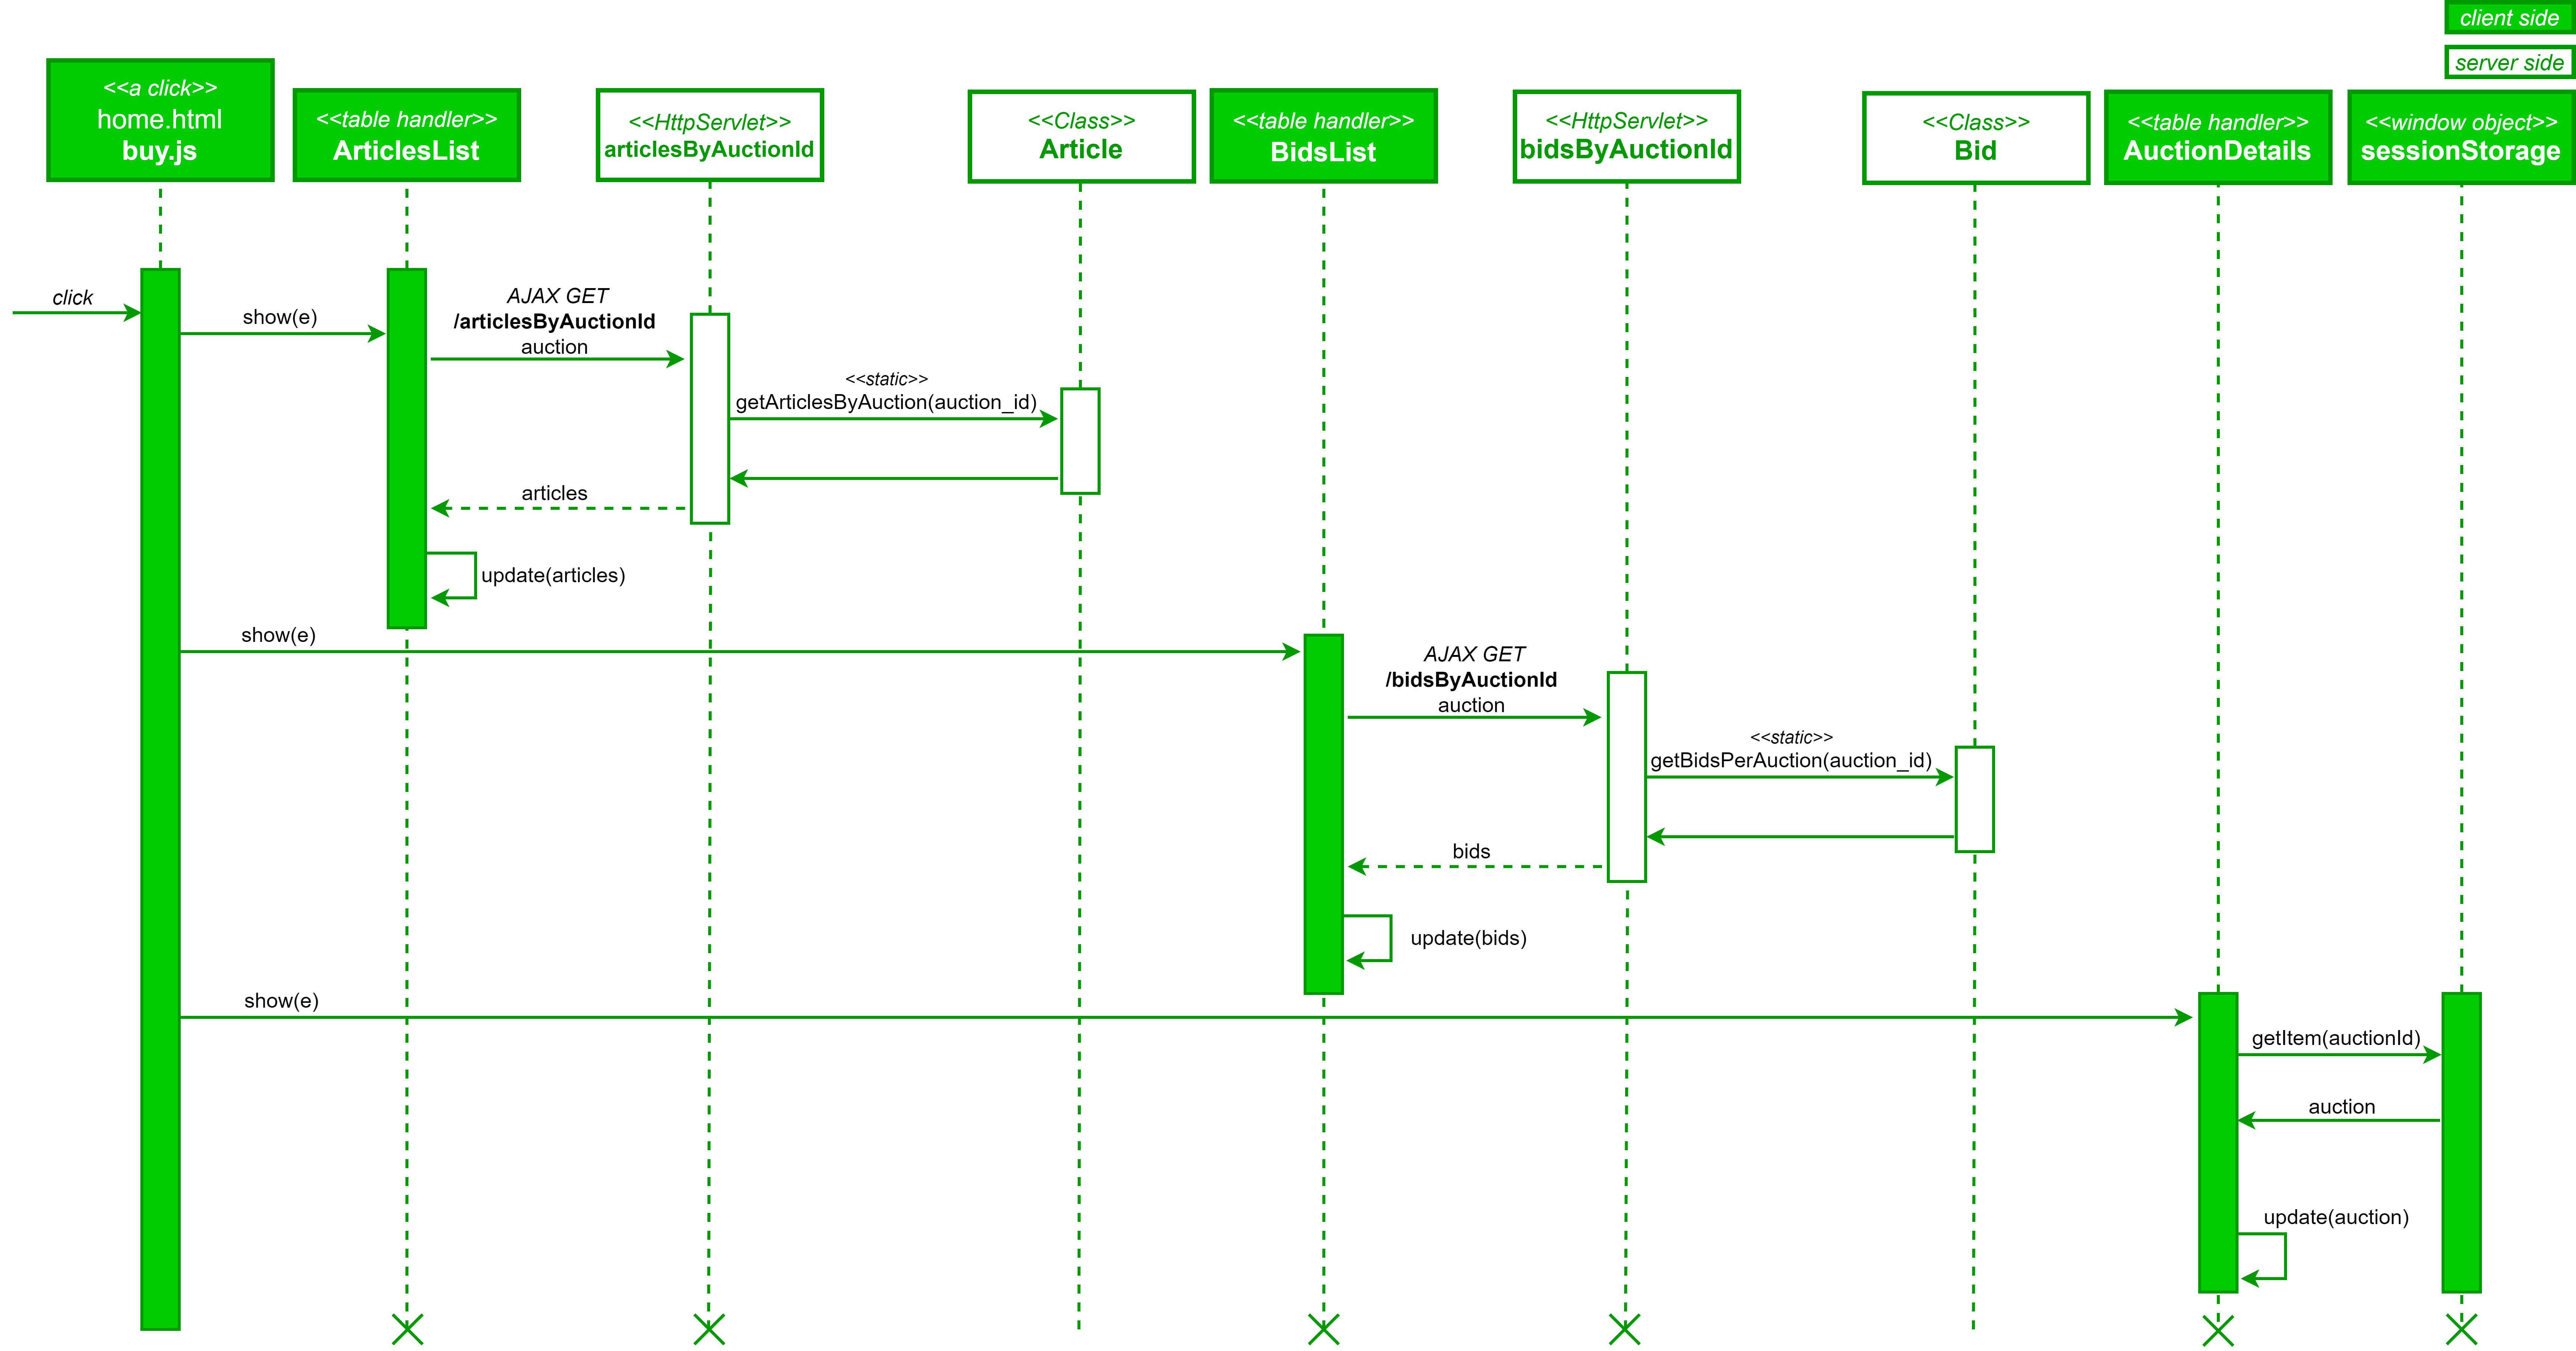
\includegraphics[width=1.2\textwidth]{RIA-SequenceDiagrams/TIWRIA-showDetails.png}}	
				\phantom{.}\\
			\subsubsection{The user places a new bid}
				\phantom{.}\\
				\noindent \makebox[\textwidth]{
					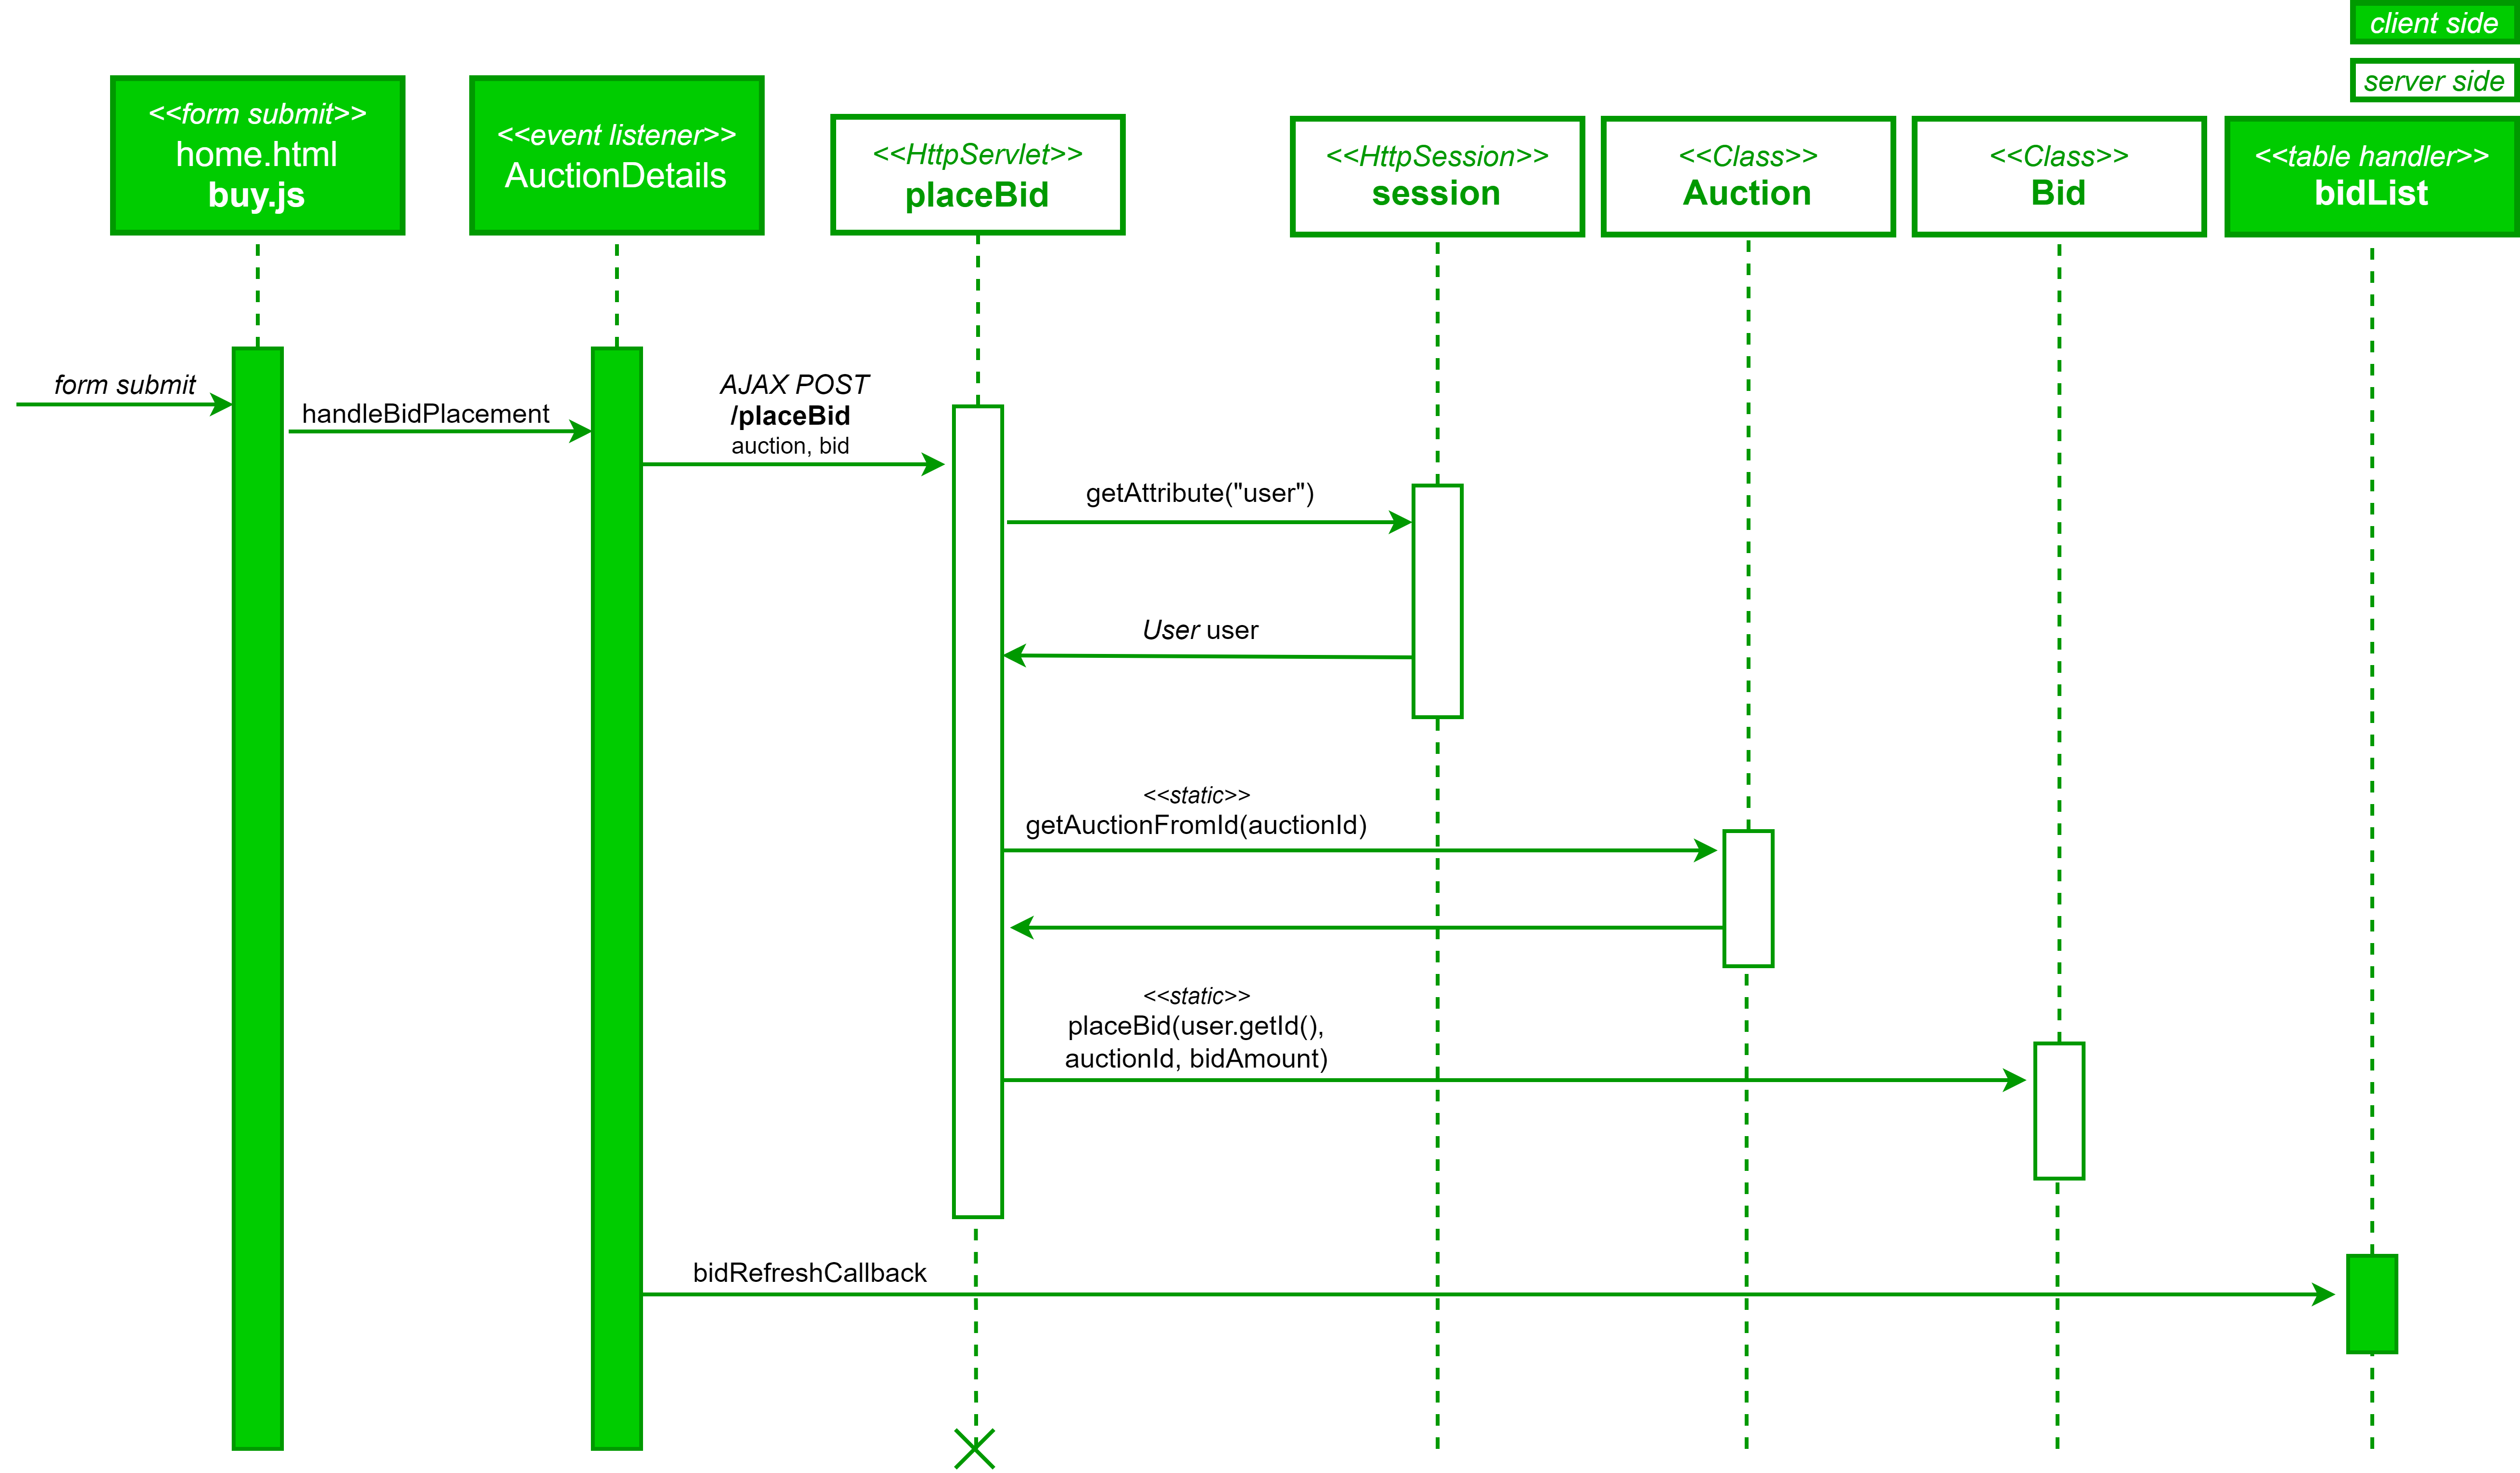
\includegraphics[width=1.25\textwidth]{RIA-SequenceDiagrams/TIWRIA-placeBid.png}}
				\newpage				
						
			\subsubsection{The user requests the SELL functionality}
				\phantom{.}\\
				\noindent \makebox[\textwidth]{
					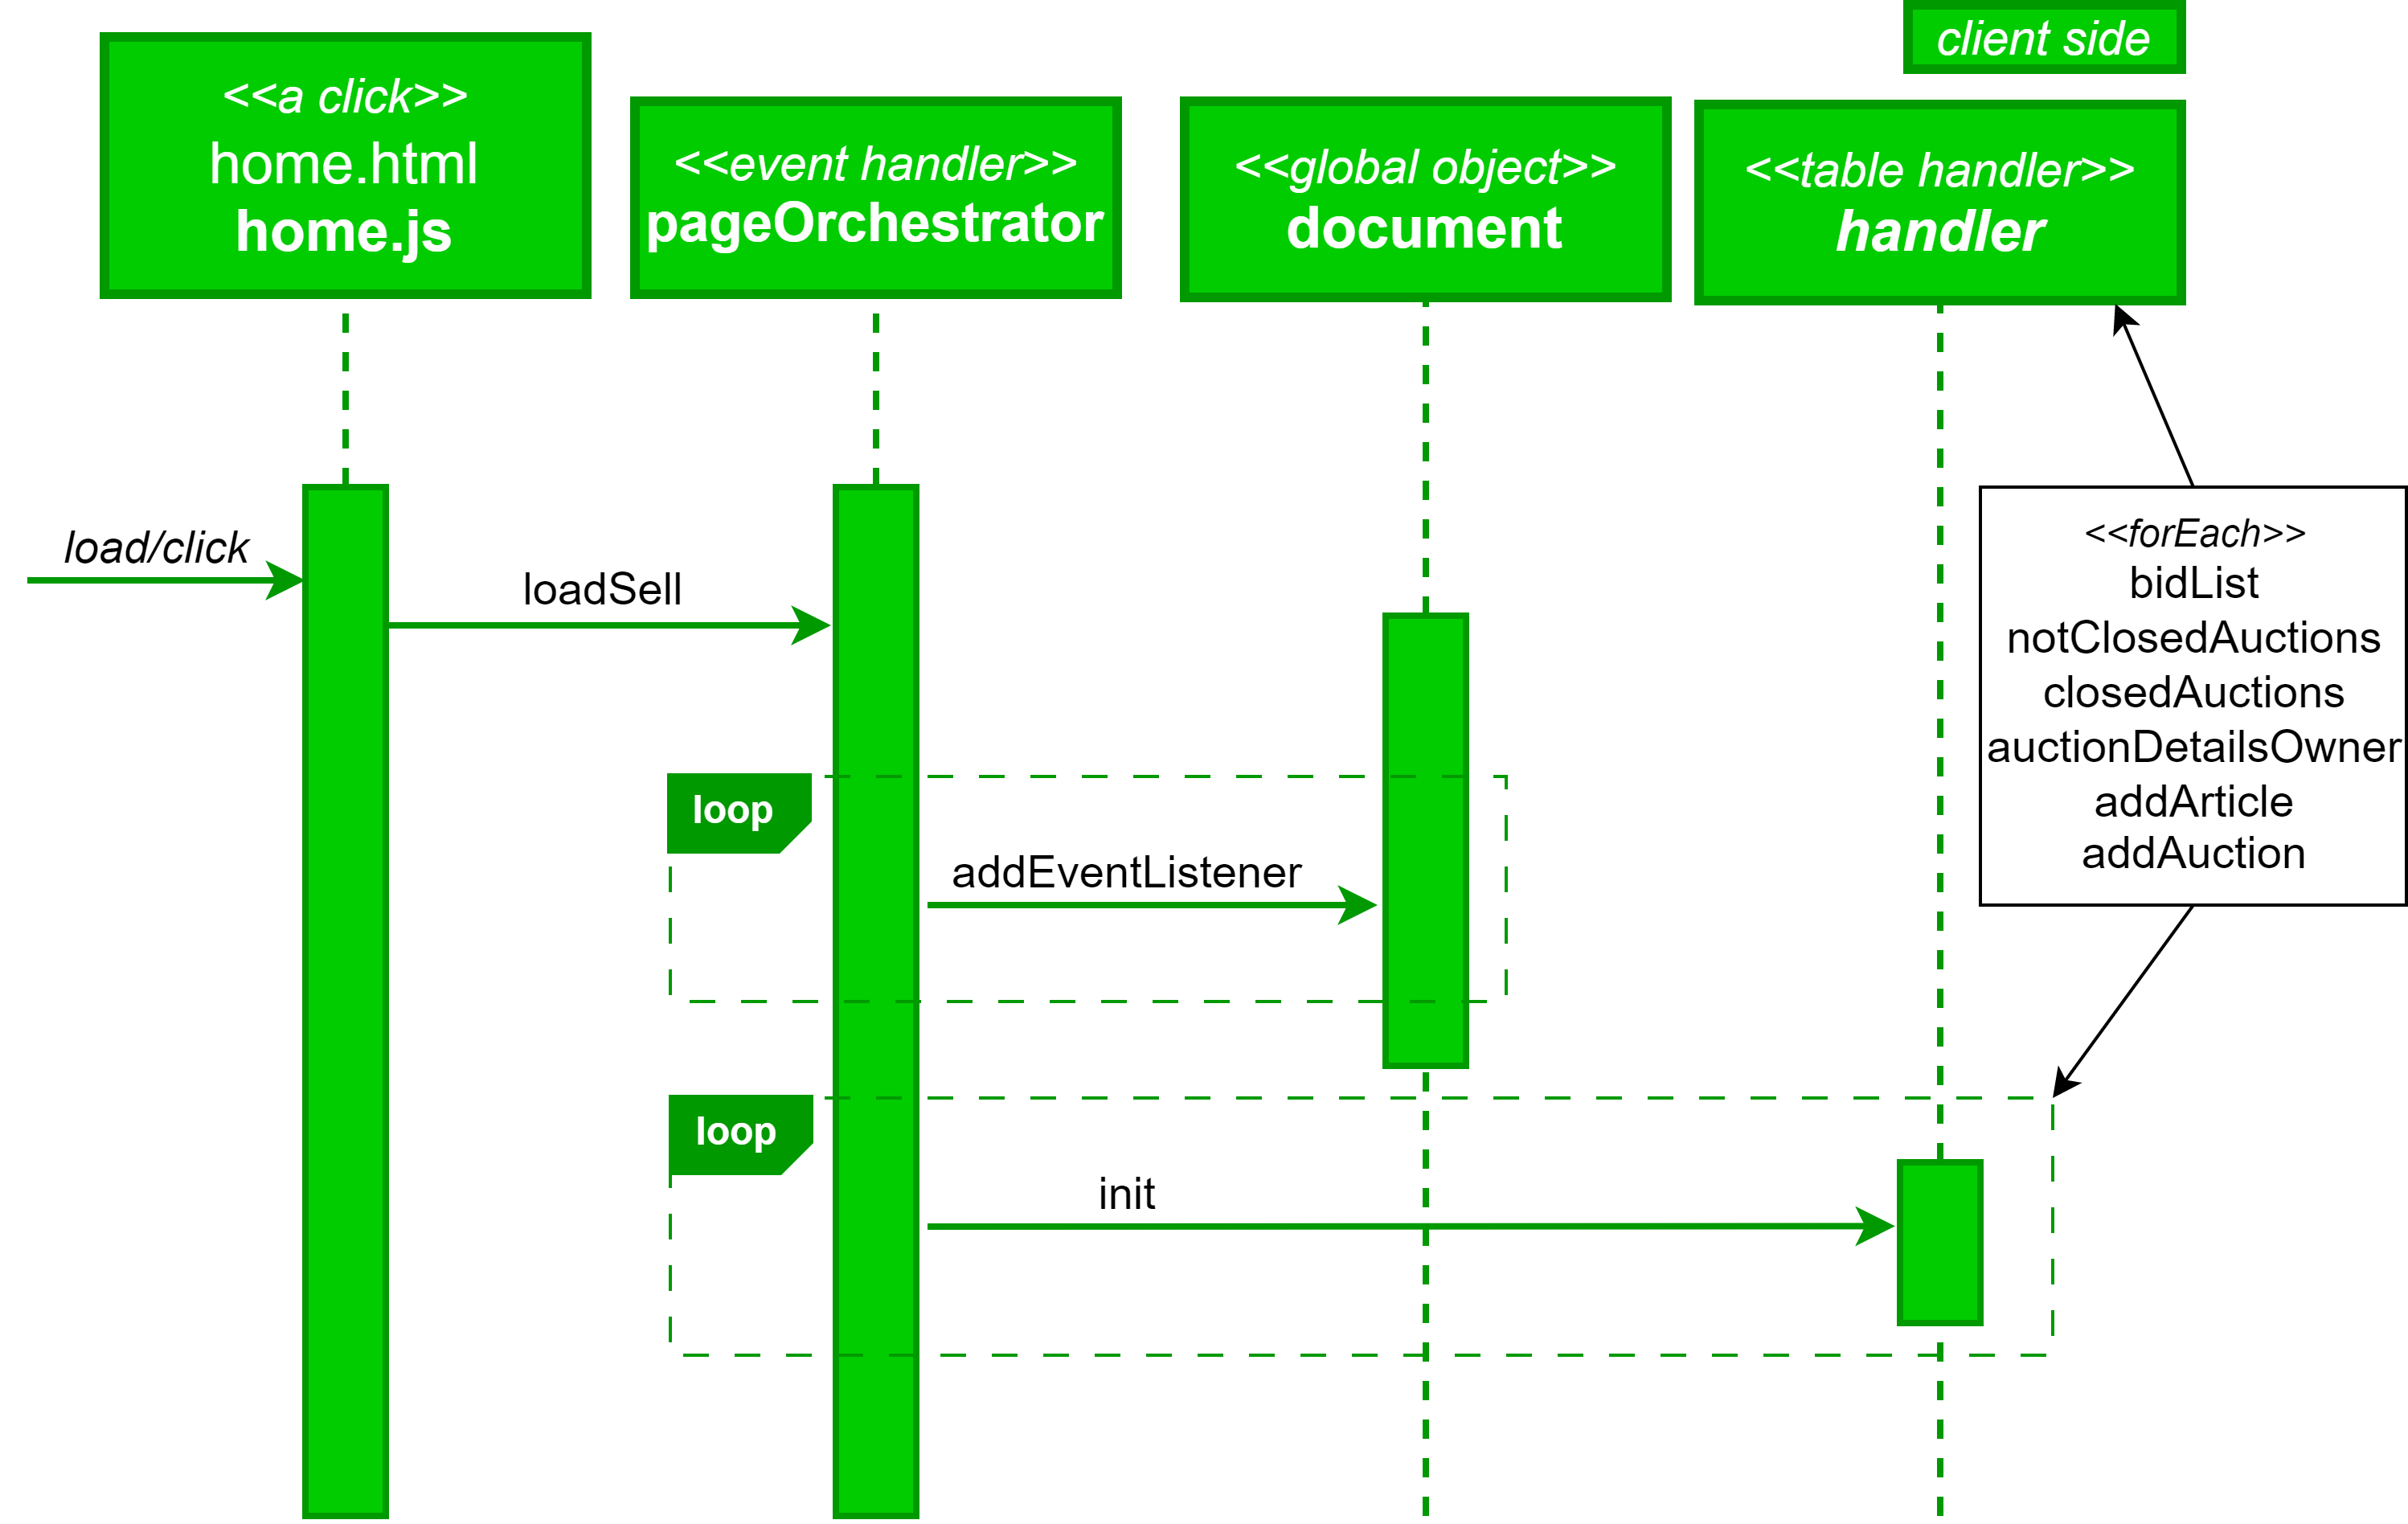
\includegraphics[width=0.9\textwidth]{RIA-SequenceDiagrams/TIWRIA-loadSell.png}}	
				\phantom{.}\\
				At the same time, both closed and open auctions are loaded. Since the sequence of operations is identical (except for one parameter, openVsClosed), only one of the two flows is shown here.
				\phantom{.}\\
				\noindent \makebox[\textwidth]{
					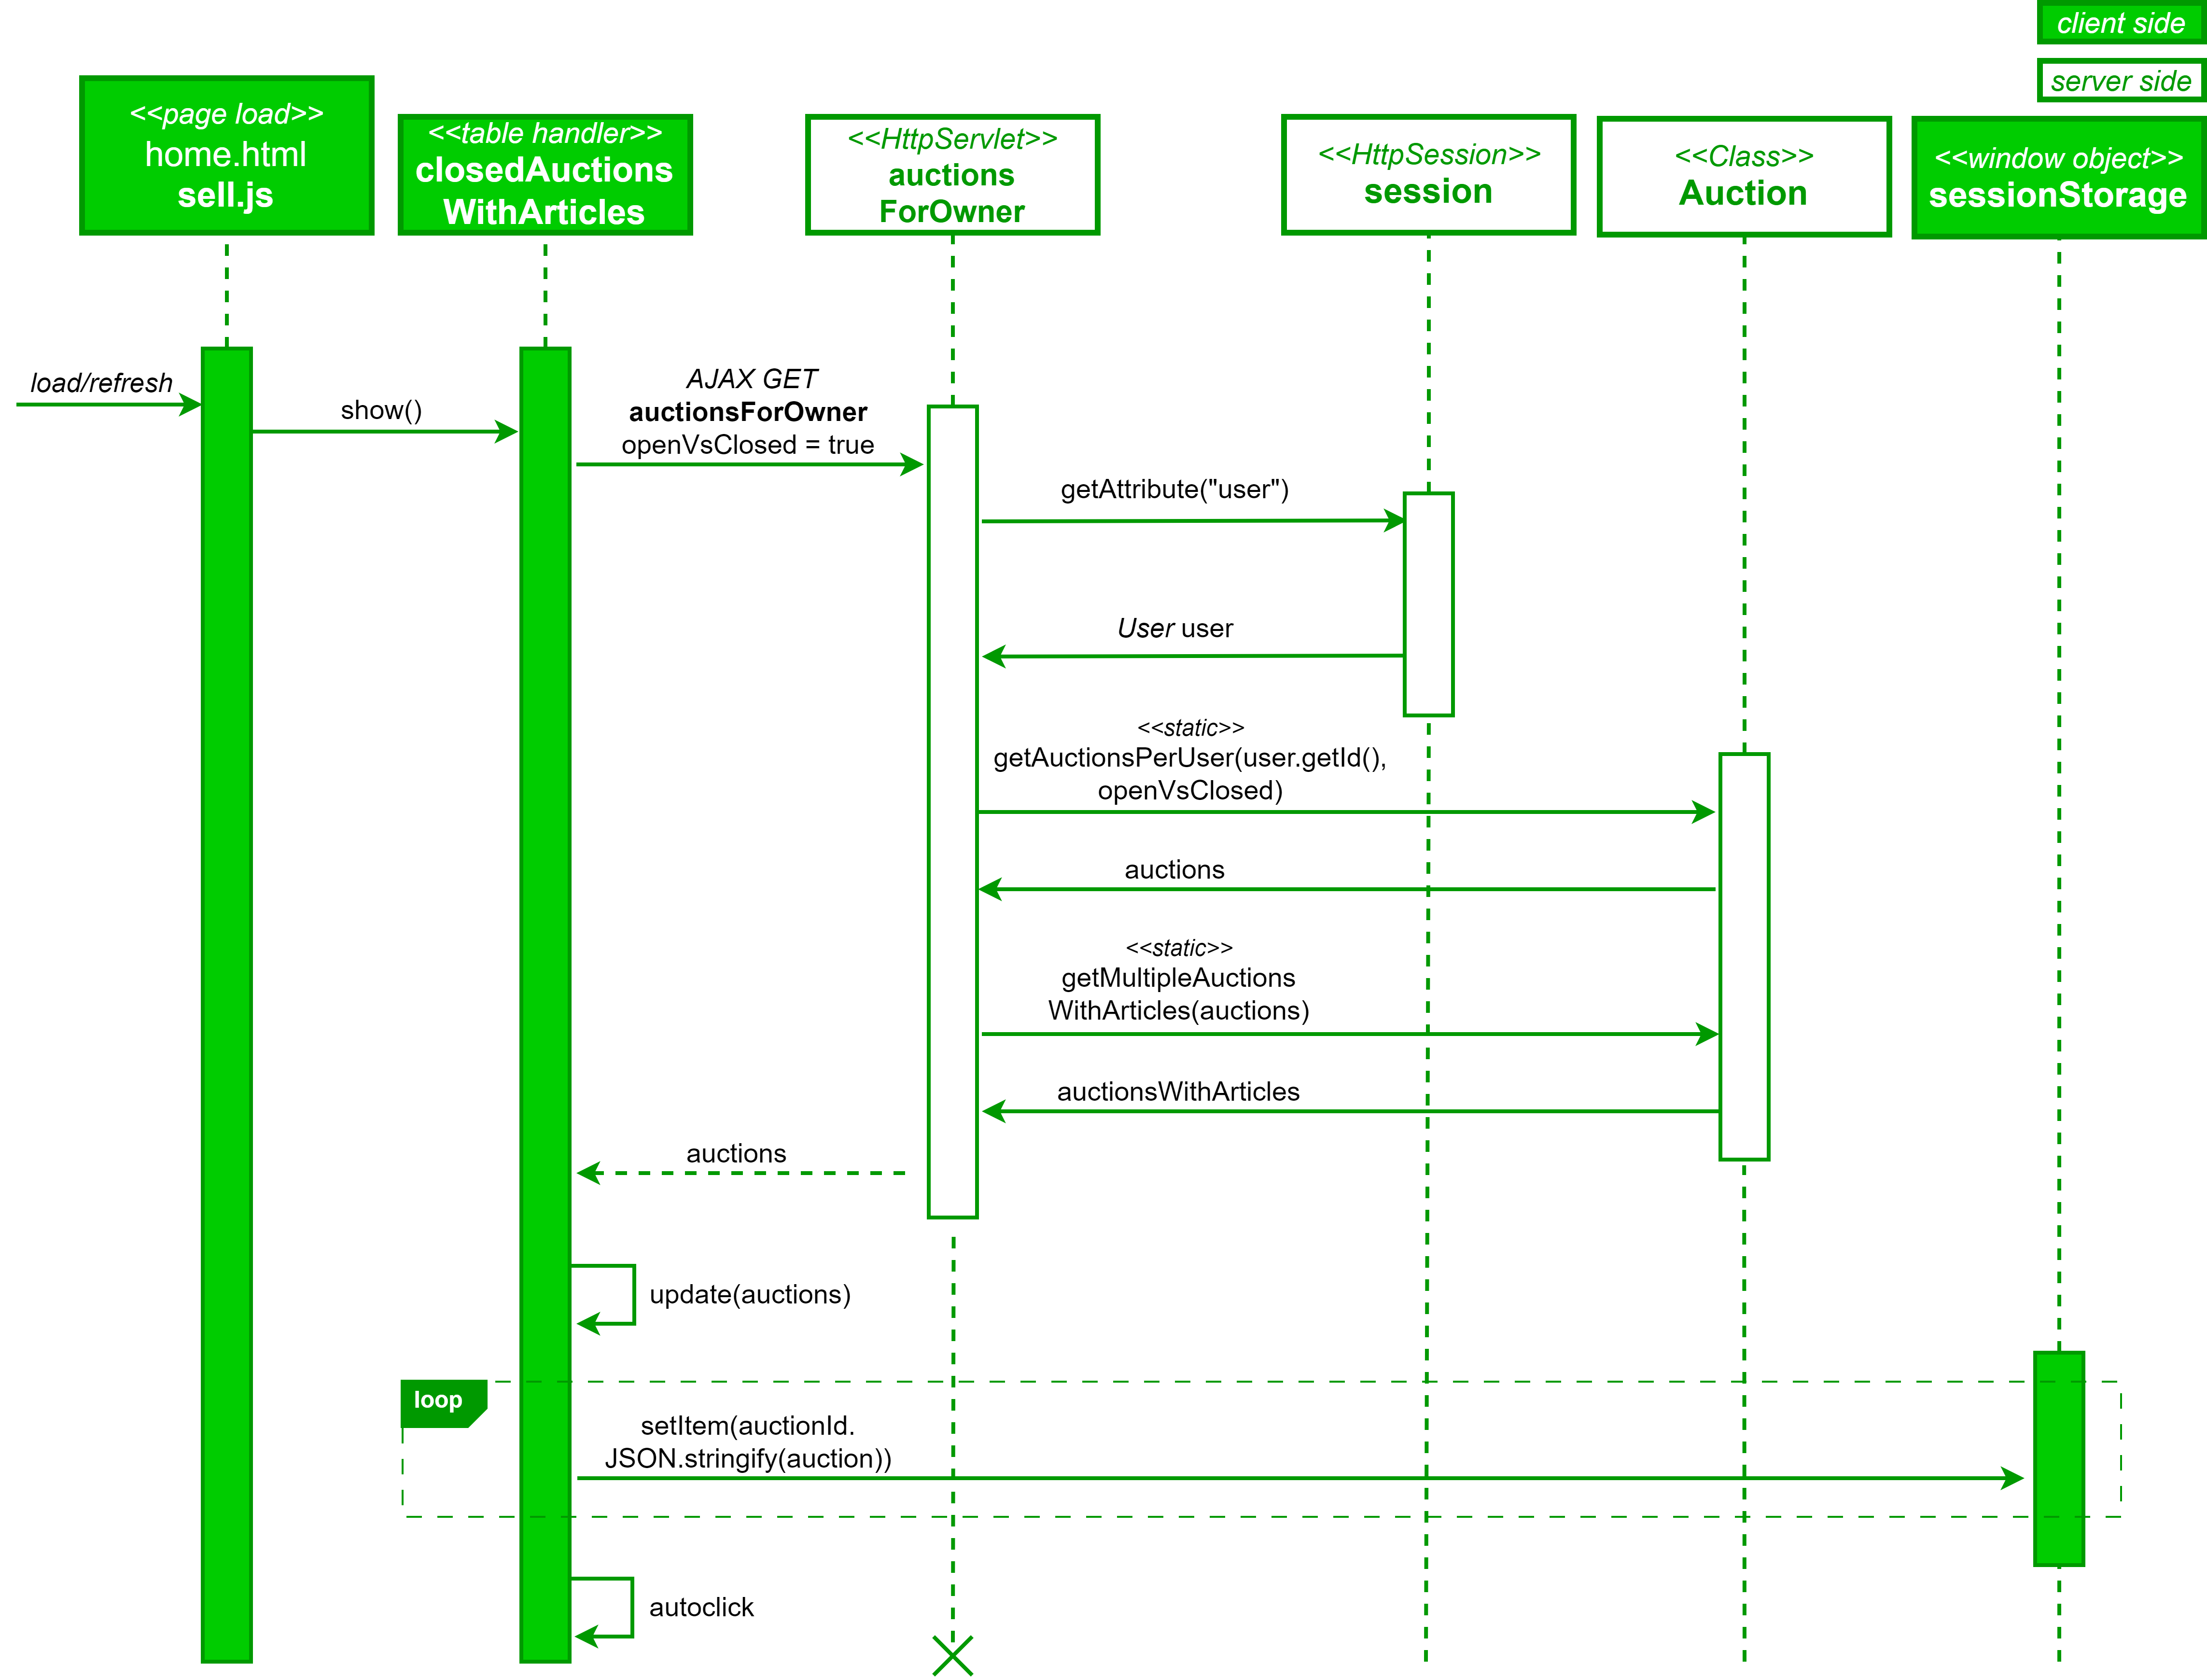
\includegraphics[width=1\textwidth]{RIA-SequenceDiagrams/TIWRIA-loadClosedAuctions.png}}	
				\phantom{.}\\
				\newpage
			\subsubsection{The user clicks to view the details of one of their auctions}
				\phantom{.}\\
				\noindent \makebox[\textwidth]{
					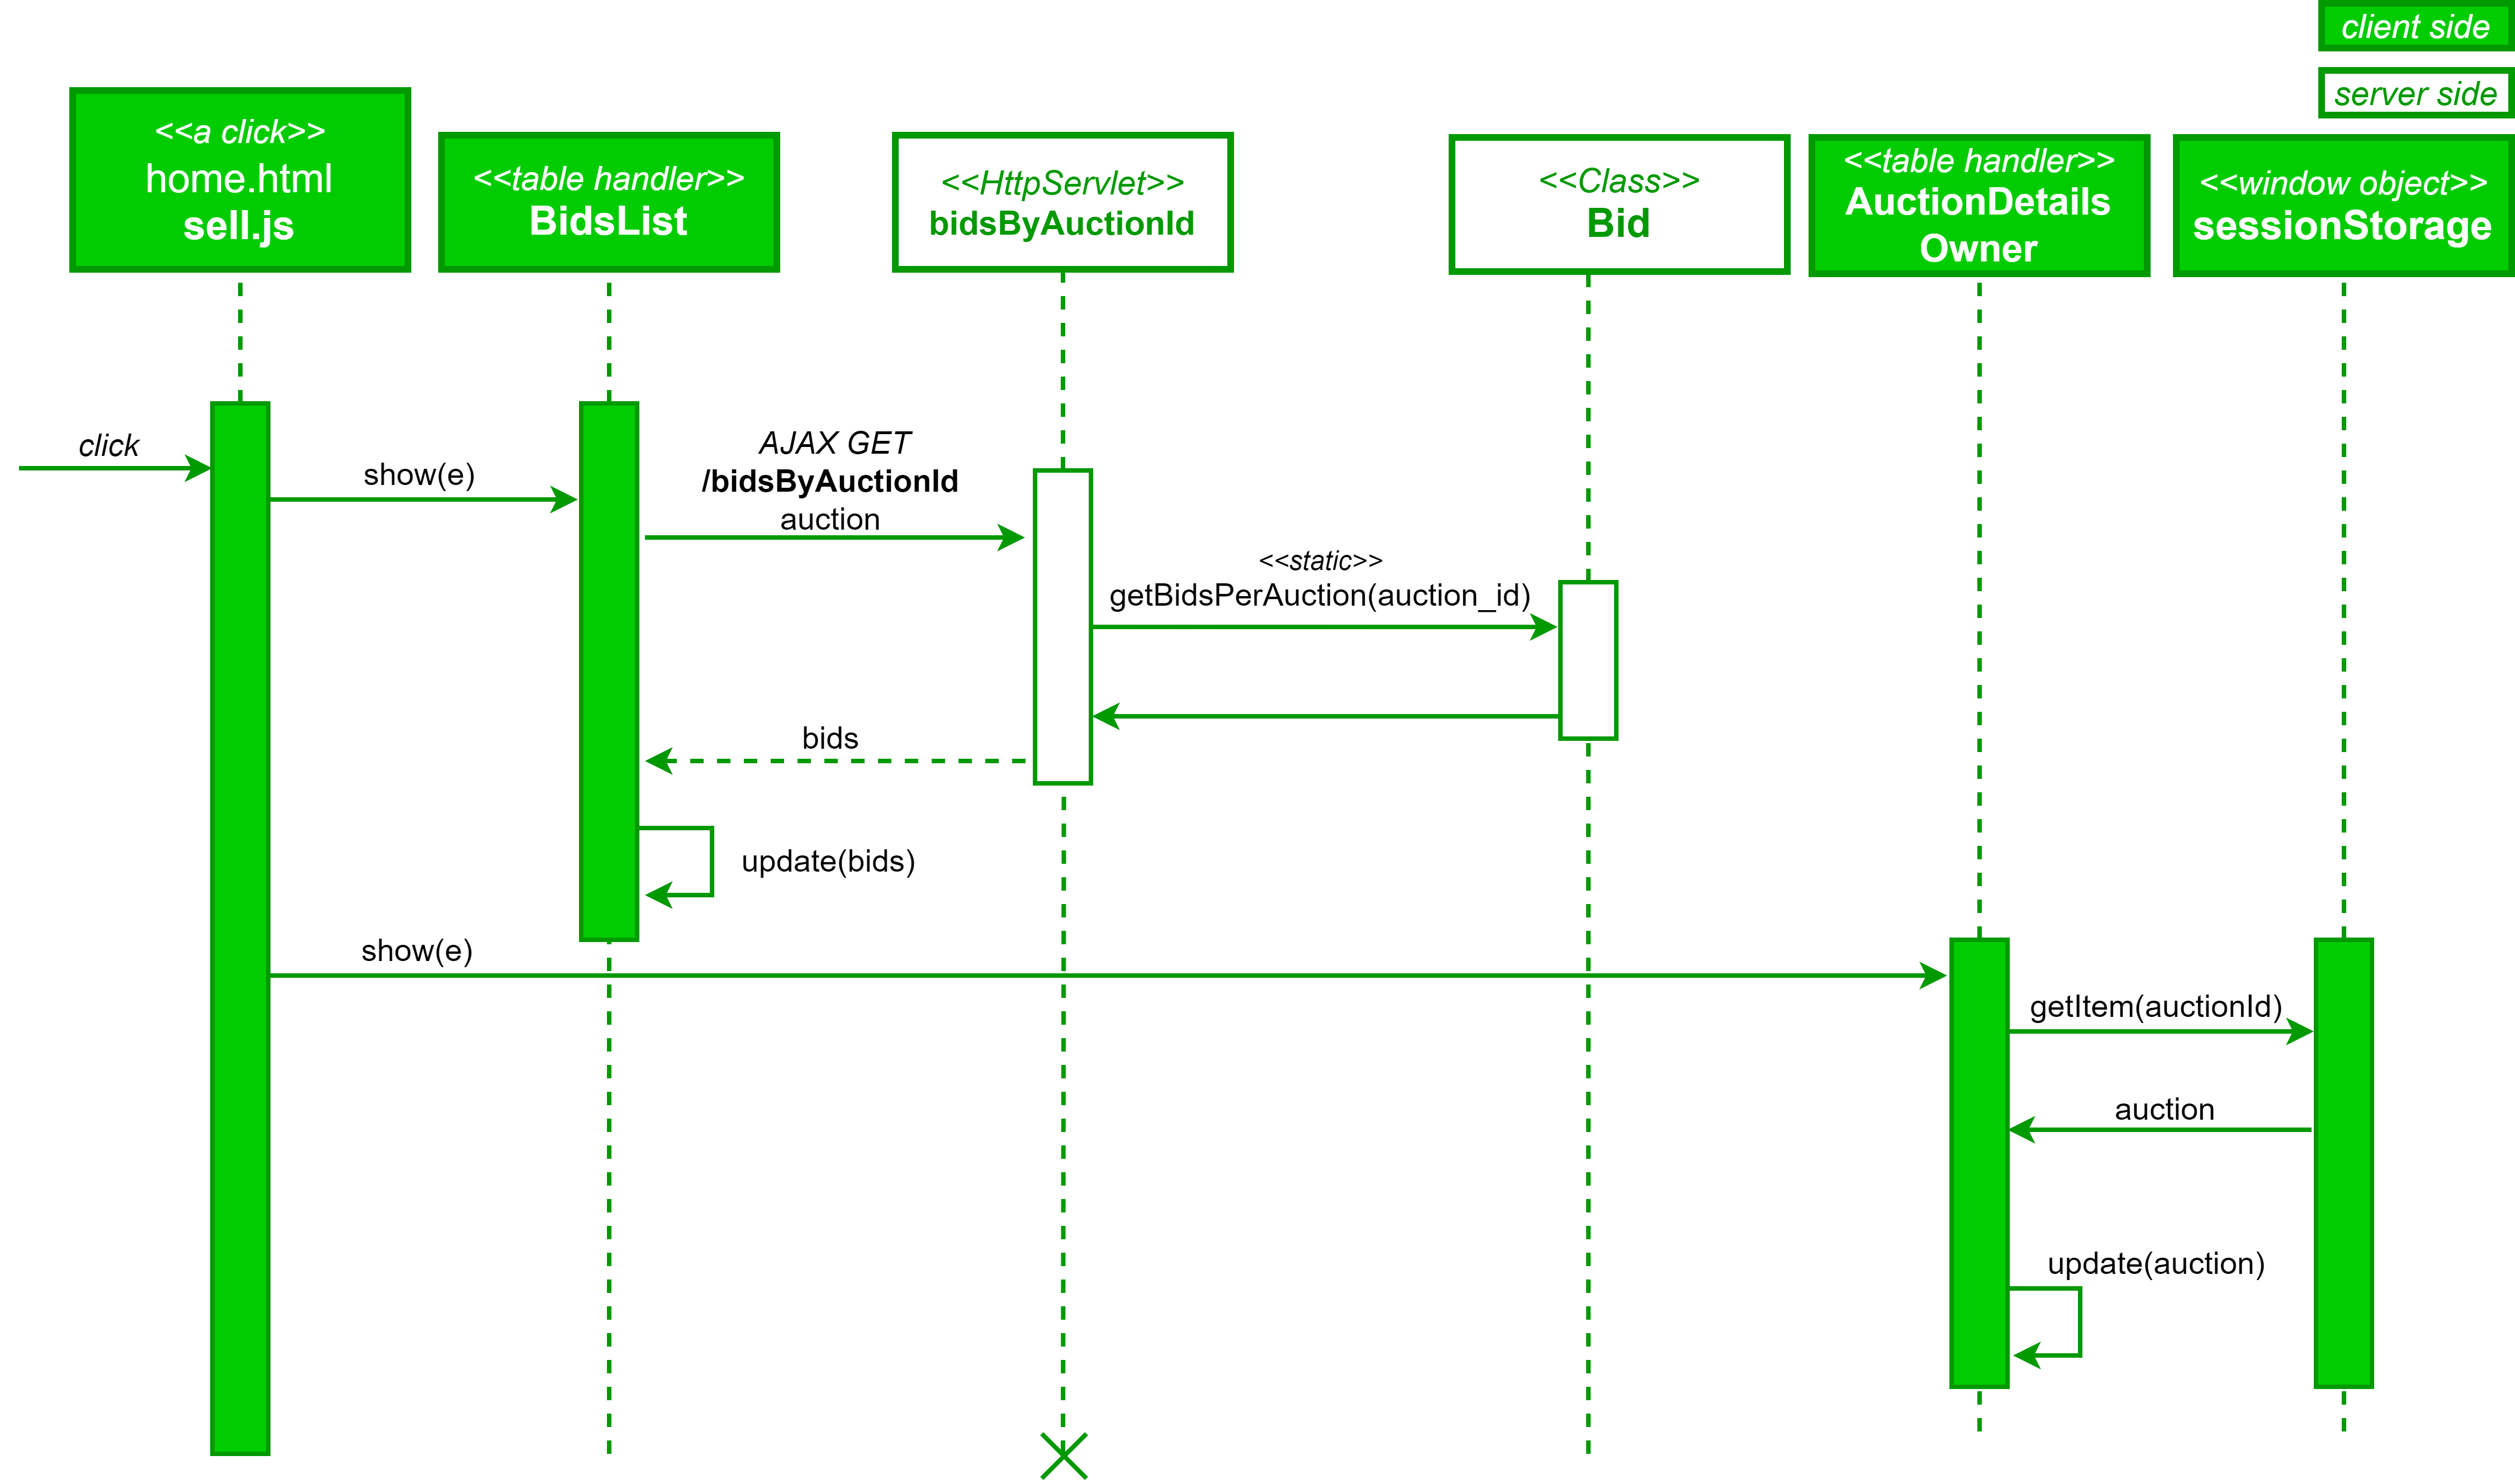
\includegraphics[width=1.25\textwidth]{RIA-SequenceDiagrams/TIWRIA-showDetailsOwner.png}}	
				\phantom{.}\\
			\subsubsection{The user uploads a new article}
				\phantom{.}\\
				\noindent \makebox[\textwidth]{
					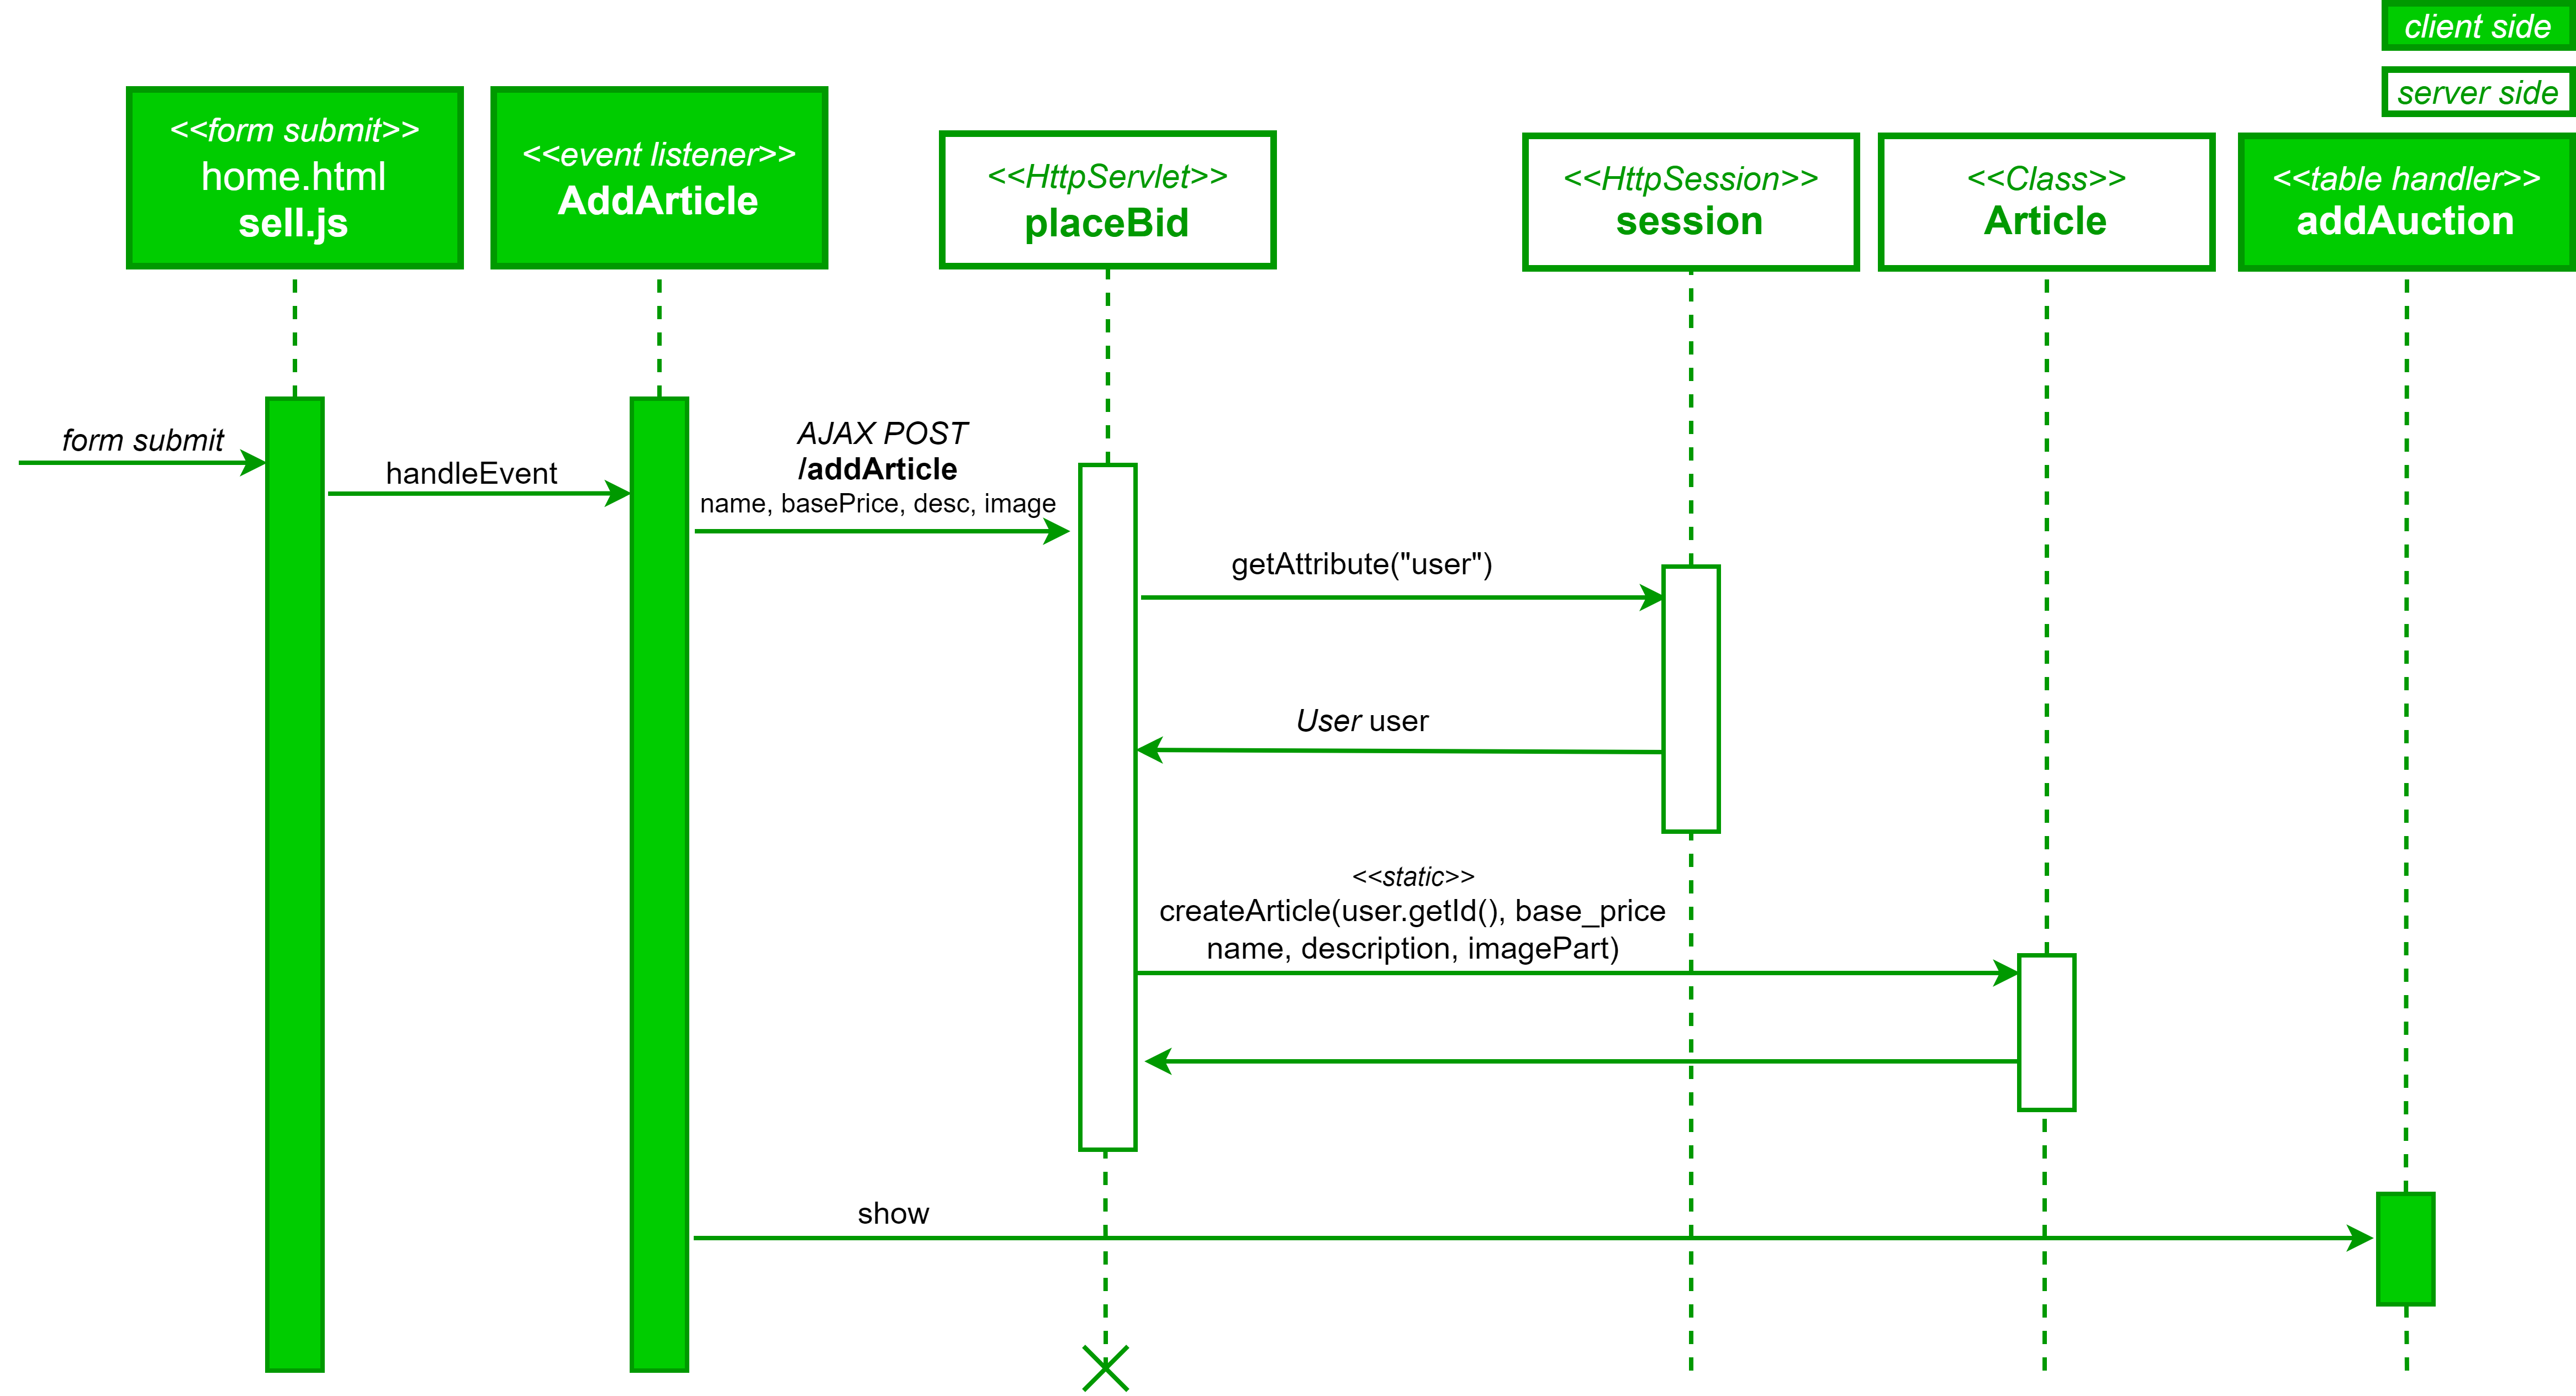
\includegraphics[width=1.1\textwidth]{RIA-SequenceDiagrams/TIWRIA-addArticle.png}}	
				\newpage
			\subsubsection{The user creates a new auction}
				\phantom{.}\\
				\noindent \makebox[\textwidth]{
					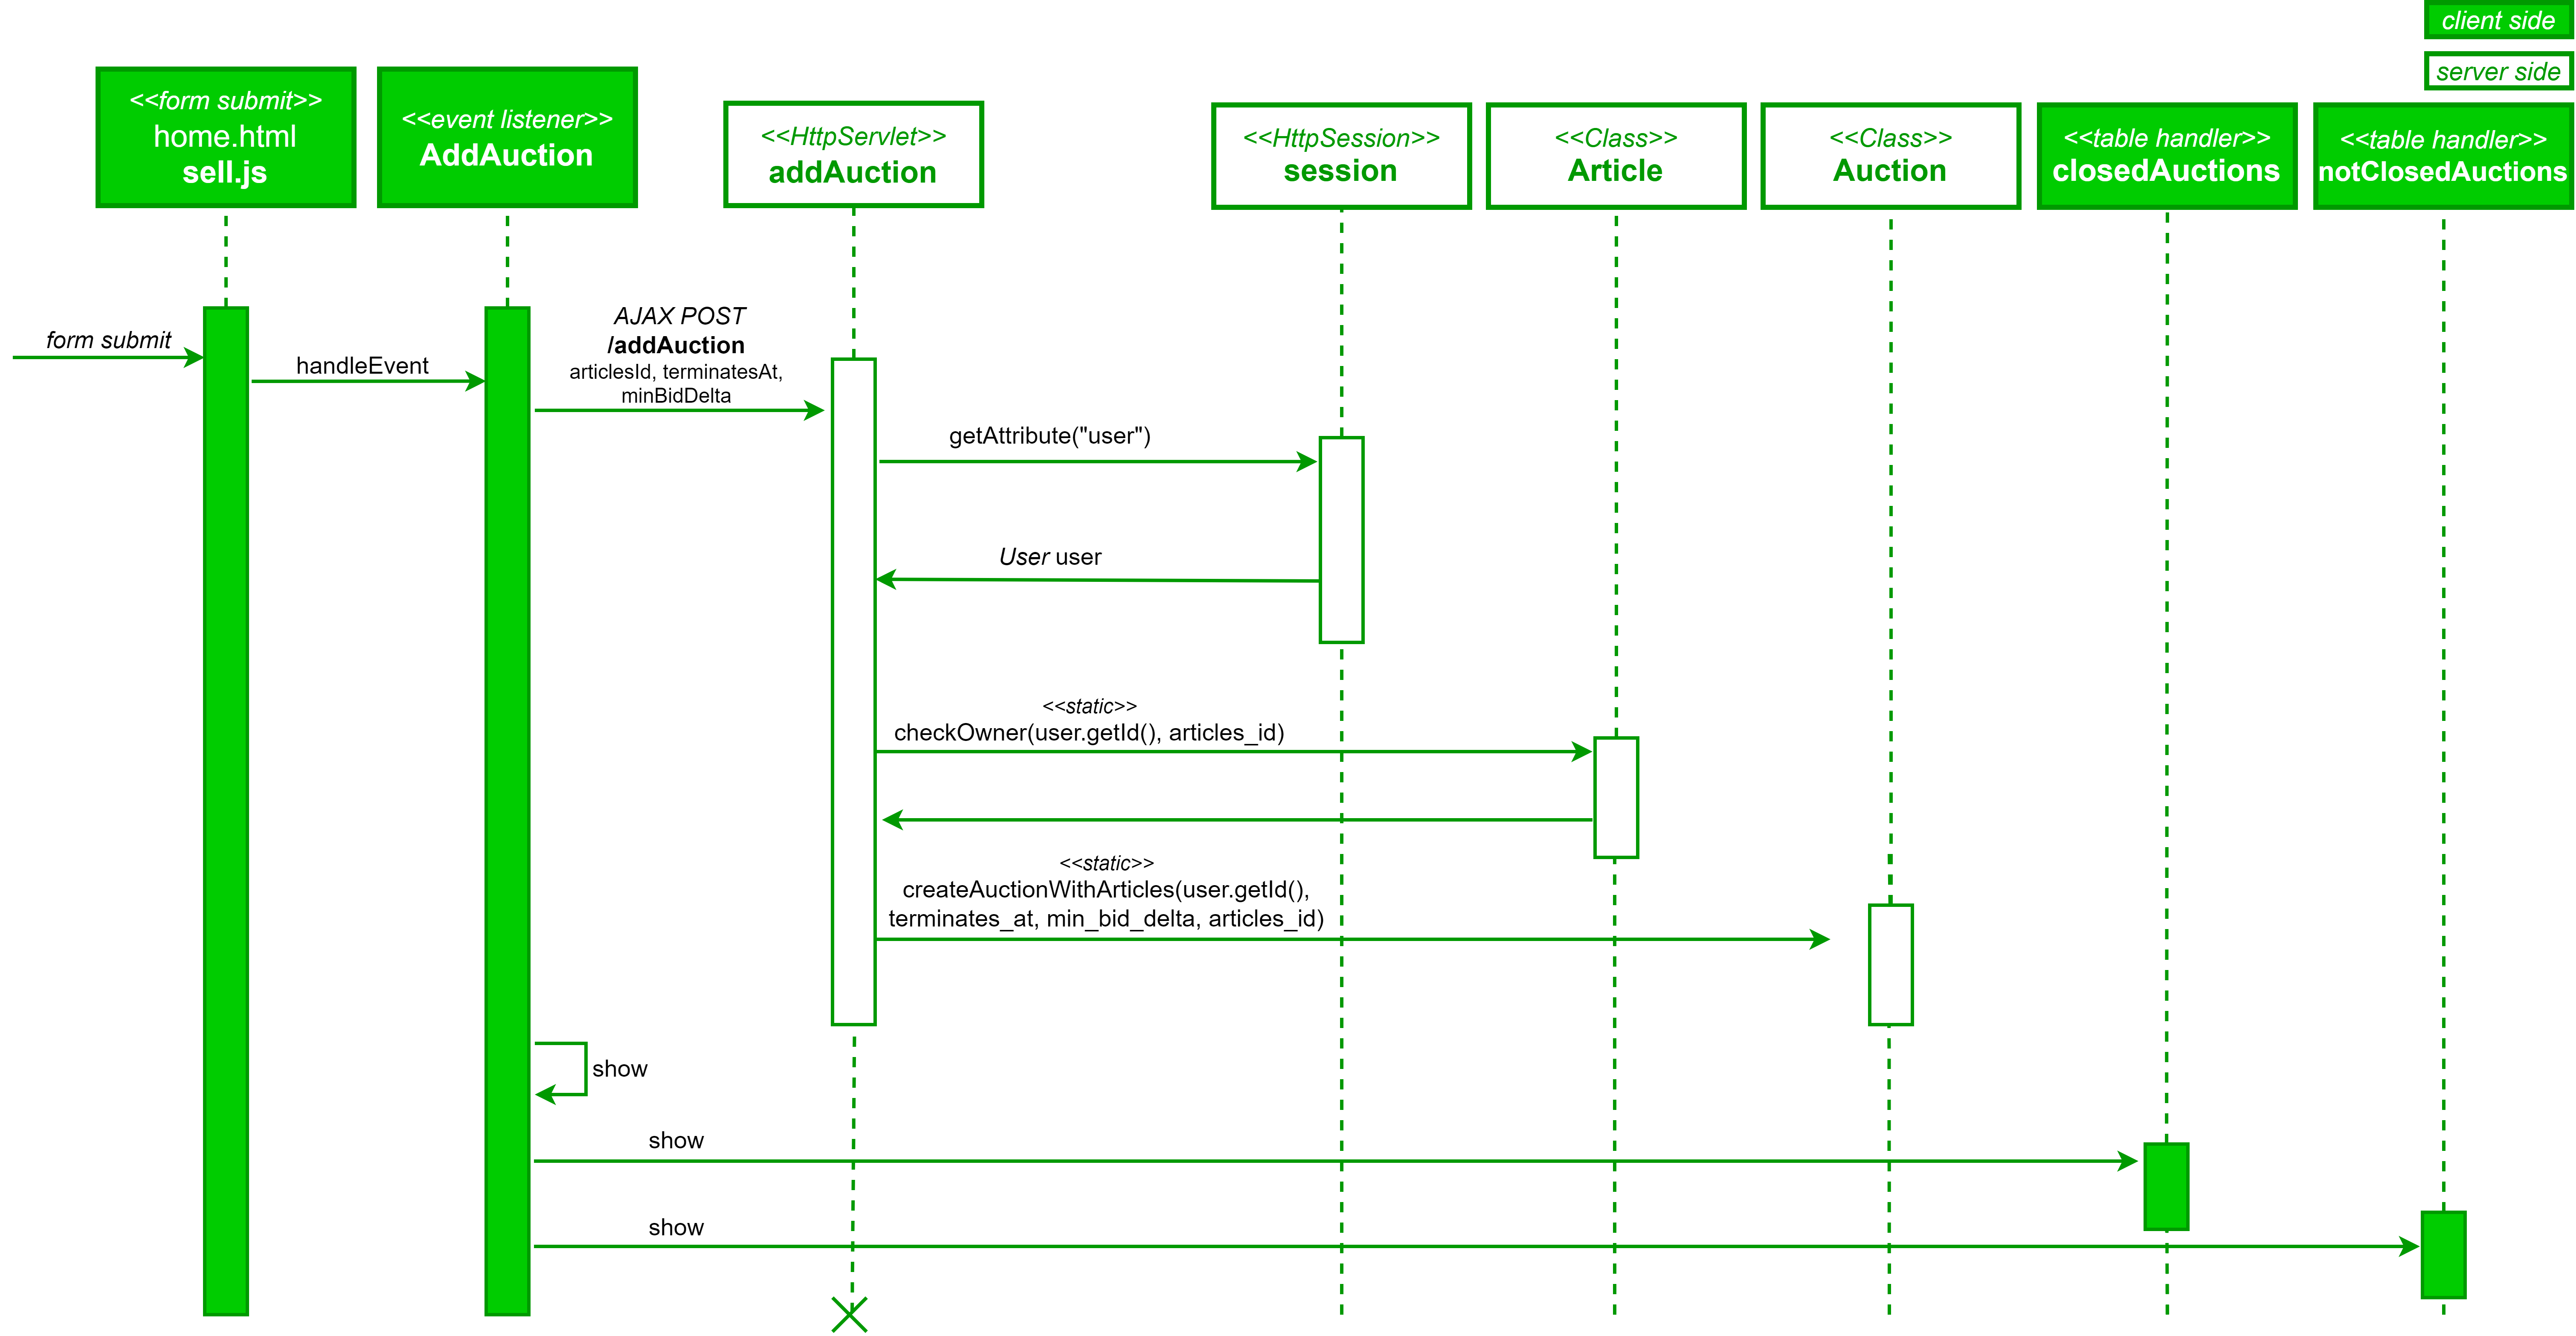
\includegraphics[width=1.25\textwidth]{RIA-SequenceDiagrams/TIWRIA-addAuction.png}}	
				\phantom{.}\\
			\subsubsection{The user closes one of their completed auctions}
				\phantom{.}\\
				\noindent \makebox[\textwidth]{
					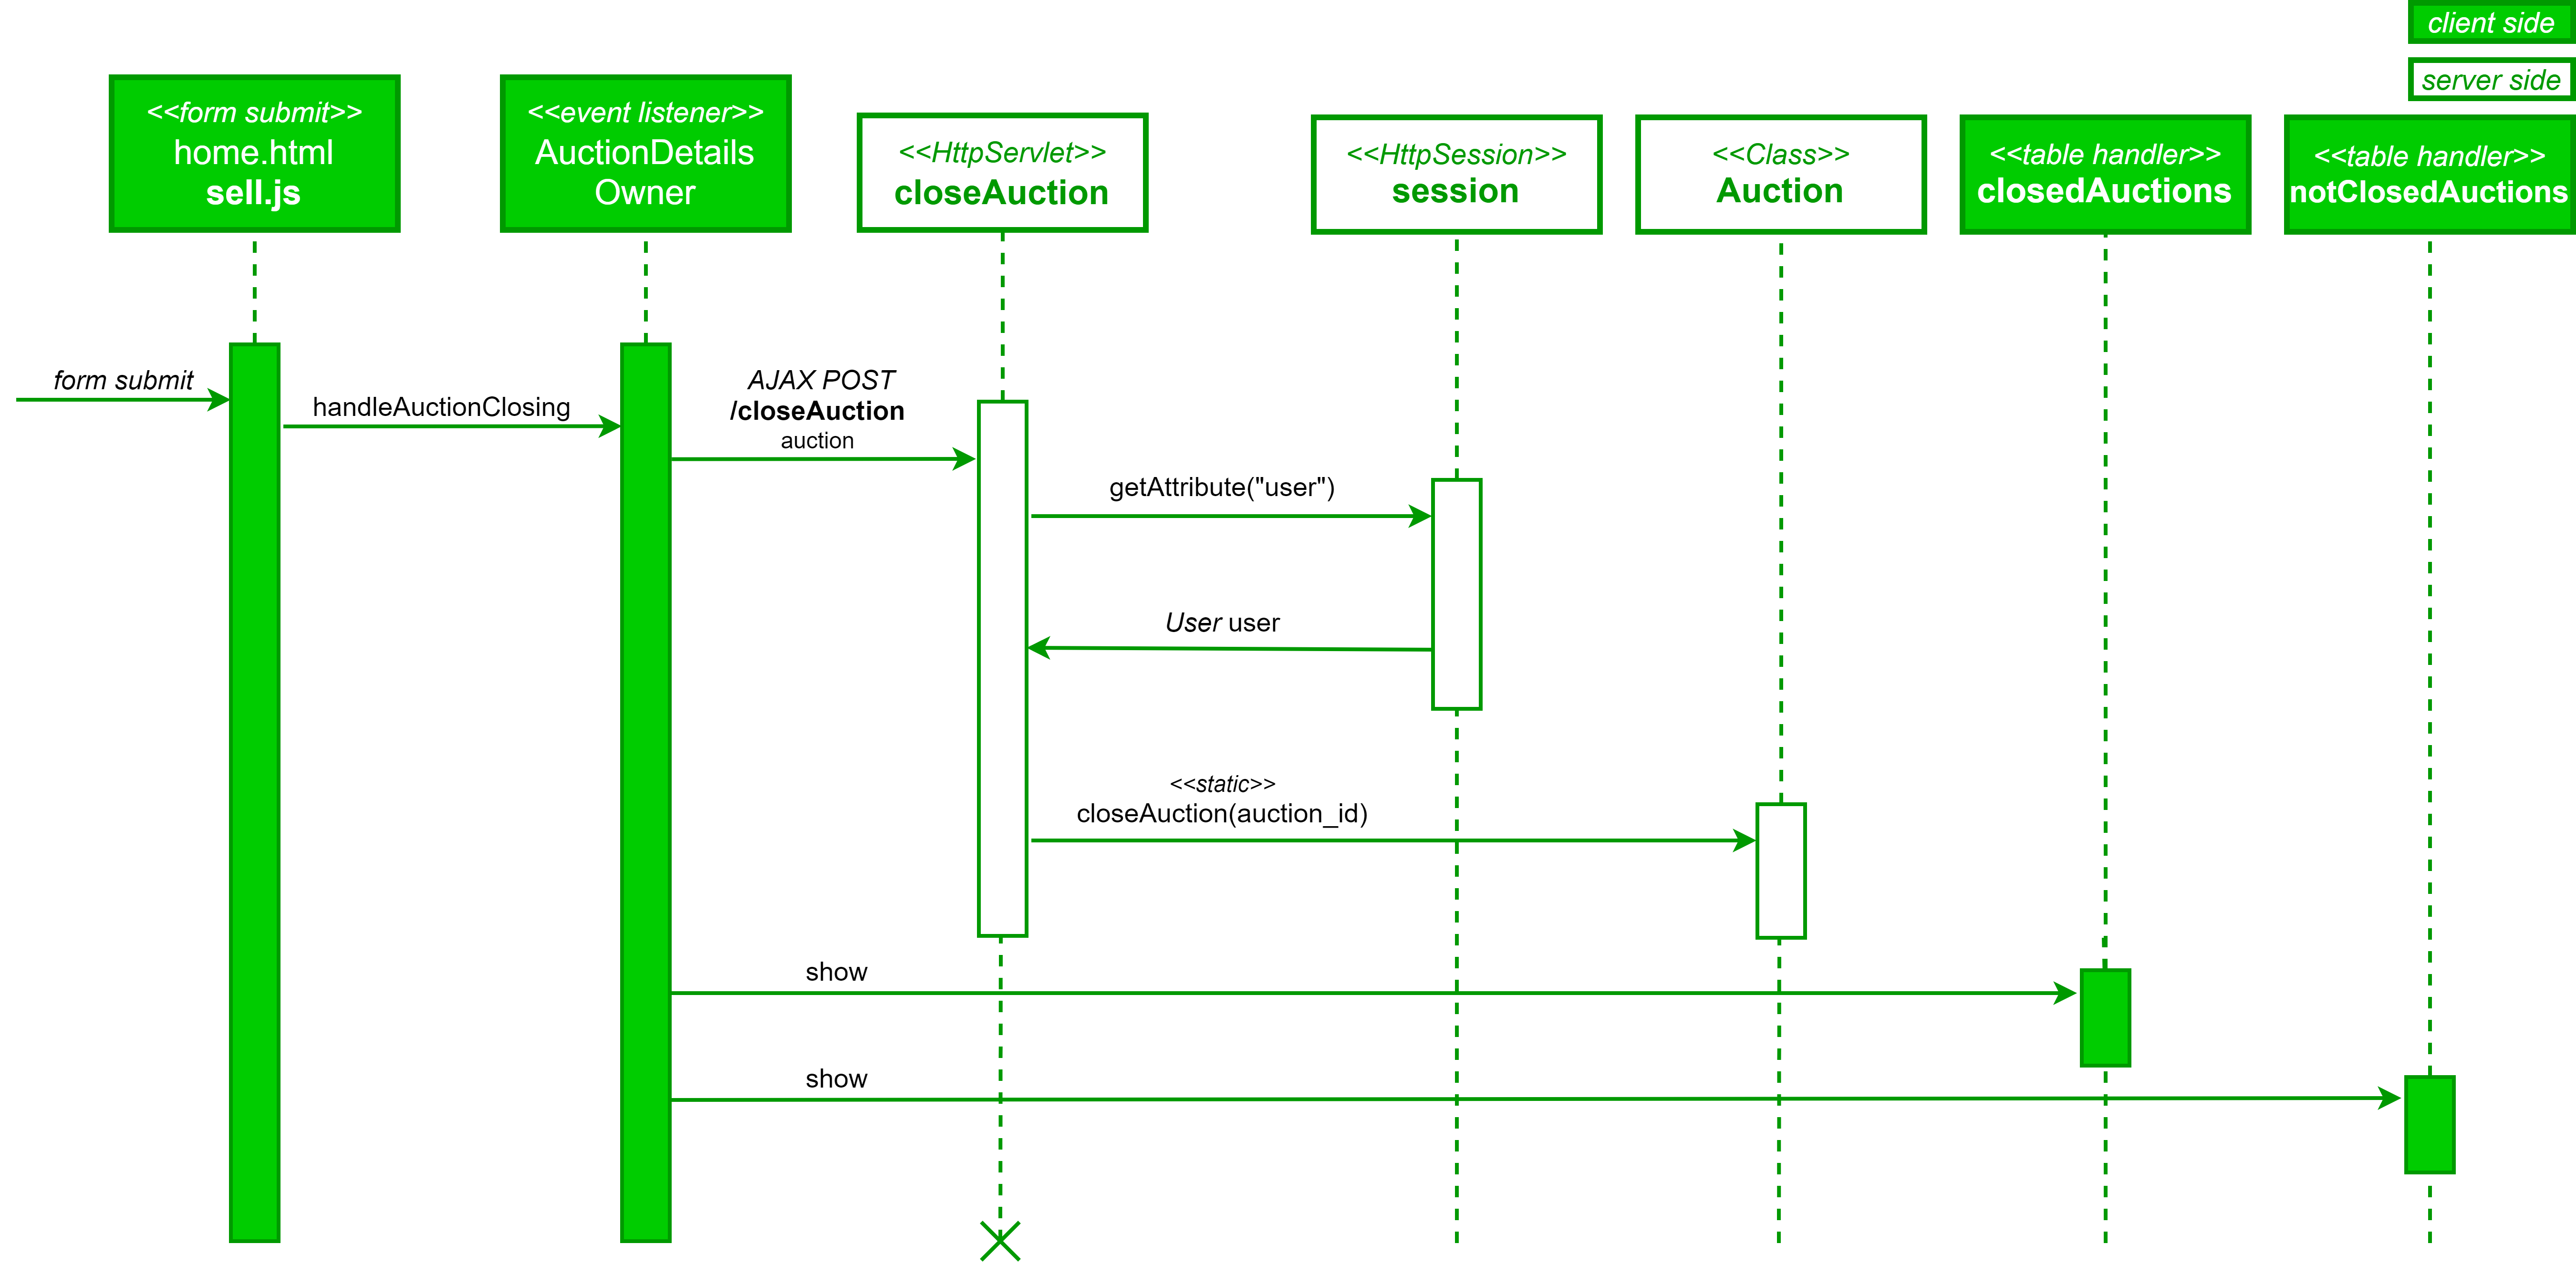
\includegraphics[width=1.2\textwidth]{RIA-SequenceDiagrams/TIWRIA-closeAuction.png}}					
				\newpage
		\section{Deployment in a Cluster with Docker and Kubernetes}
		\lstset{language=XML}
		For demonstration purposes, this project has been deployed in a Kubernetes (k8s) cluster to be publicly accessible on the web. This section outlines some of the key steps to achieve this goal, as well as some additional configurations required to support this type of deployment compared to a demo version.

		\subsection{Interactions with the Database}
		Interacting with a production database, as opposed to a local testing database, requires that:
		\begin{itemize}
		    \item Connections do not remain open beyond a certain timeout, managed by the DBMS;
		    \item Since opening connections is resource-intensive, connections should be requested as infrequently as possible and shared among servlets;
		    \item It should be verified that the active connections have not been closed unexpectedly;
		    \item The application must be robust against unexpected \textit{SQLException}s thrown due to network errors;
		    \item Database credentials should be stored as securely as possible, certainly not alongside the application code.
		\end{itemize}
		To meet the first three requirements, the connection management logic was delegated to a \hyperref[accessodb]{ConnectionHandler} class, as detailed in the corresponding section. Regarding credentials, they should be read through environment variables, enabling integration with Kubernetes Secrets and standard access mechanisms for protected resources within the cluster.

		\subsection{Caching of Content}
		To minimize network traffic, Tomcat has been configured so that static content is cached locally in the browser. 

		For the pure HTML version, only the CSS stylesheet can be cached since all HTML pages contain dynamically generated content. In the JavaScript version, this can be optimized much further: all the JavaScript code, HTML markup, and CSS can be requested only on the first connection and cached by the browser. Additionally, the use of session storage allows auction information to be requested only when strictly necessary.

		To properly instruct the browser on using the cache, some HTTP headers need to be set. This is handled by an \textit{ExpiresFilter} provided by Apache Catalina. The configuration for this filter, which is inserted in the web.xml file, is as follows:

		\begin{lstlisting}
		    <filter>
			<filter-name>ExpiresFilter</filter-name>
			<filter-class>org.apache.catalina.filters.ExpiresFilter</filter-class>
			<init-param>
			    <param-name>ExpiresDefault</param-name>
			    <param-value>access plus 30 minutes</param-value>
			</init-param>
			<init-param>
			    <param-name>ExpiresByType application/json</param-name>
			    <param-value>access plus 0 seconds</param-value>
			</init-param>
		    </filter>
		    <filter-mapping>
			<filter-name>ExpiresFilter</filter-name>
			<url-pattern>*</url-pattern>
			<dispatcher>REQUEST</dispatcher>
		    </filter-mapping>
		\end{lstlisting}

		\subsection{Protection Against Brute-Force Attempts}
		There are several configurations to protect the application from malicious access attempts. To integrate with the existing architecture in the used cluster, logs are utilized as an interface: each access attempt is logged in the Tomcat logs so that this information can be analyzed by an intrusion prevention system such as Crowdsec. Within a Kubernetes cluster, logs must be written to stdout so that they can be consulted and made available to other pods. Therefore, it is necessary to modify Tomcat's configuration to add stdout output to the default logging pipeline (which writes to file).

		\subsection{Protection of Passwords}
		It is always good practice not to store user credentials in plaintext, so the $SHA1$ hashing algorithm is used to store passwords in the database. This is slightly more robust than $MD5$ (and other even weaker algorithms) while still having an acceptable computational cost. Using more complex algorithms such as $SHA256$ or $SHA512$ would make the application more vulnerable to denial-of-service attacks on machines with lower computational power, and is deemed excessive for demonstration purposes.

		\subsection{Session Distribution Across Multiple Nodes}
		Within a k8s cluster, HTTP requests are managed by load-balancing mechanisms (partially provided by an external load balancer, partially by Kubernetes Services) and reach a different Tomcat process each time. To ensure the user is properly recognized, the session content used by the servlets must be replicated across each instance. Tomcat provides clustering functionality to support this need, allowing configuration of how each Tomcat process can reach others on different nodes and how replication should occur. For this demonstration, each time a modification is made to the session, the delta is sent to all nodes.

		By using the k8s StatefulSet resource to manage the pods, it is possible to address other containers in the set using Kubernetes' internal DNS resolution. The DNS name format is as follows: $nomePod-N.nomeSet.namespace.svc.cluster.local$. This is part of the necessary configuration, specifying how to reach Pod 1:

		\begin{lstlisting}
		    # Addressing other pods using internal DNS resolution
		    <Member className="org.apache.catalina.tribes.membership.StaticMember"
		    port="4000"					
		    host="tiw-project-0.tiw-project.default.svc.cluster.local"  # Pod 1			
		    uniqueId="{0,1,2,3,4,5,6,7,8,9,10,11,12,13,14,15}"/>  # Random
		\end{lstlisting}

		Alternatively, it would have been possible to store session content in the DB, associating a random string with each client, stored in the browser's cookies, and manually implementing the mechanism to reconstruct the session from the cookie.

		\subsection{Building the Docker Image and Deployment}
		For the application to be deployed, it is necessary to "build" a Docker image that contains Tomcat, the Java code, and the resources (configurations are inserted into the container at runtime). To do this, we use the base Tomcat image from DockerHub and add the .war file compiled by the IDE to this image. The following Dockerfile contains all the necessary instructions:

		\begin{lstlisting}
		    FROM tomcat:10.1.8
		    LABEL maintainer="dudoleitor@dudoleitor.com"
		    ADD tiw.war /usr/local/tomcat/webapps/ROOT.war
		    RUN chown 65210:65210 -R /usr/local/tomcat/
		    RUN mkdir /data
		    RUN chown 65210:65210 /data
		    EXPOSE 8080
		    USER 65210
		    CMD ["/usr/local/tomcat/bin/catalina.sh", "run"]
		\end{lstlisting}

		This image must then be uploaded to a Docker registry so that it can be downloaded by the cluster nodes. The operations for building the image, uploading it, and restarting the resources in the cluster are automated using Apache Maven.

		To complete the deployment, the following steps are taken:

		\begin{itemize}
		    \item Define the StatefulSet resource, which specifies the details of the containers (environment variables, mounted folders, hardware resource limits, privileges, etc.);
		    \item Add a Secret with database access credentials;
		    \item Add a ConfigMap for Tomcat configurations;
		    \item Prepare a persistent volume to store files (e.g., item images);
		    \item Define a Service to expose the pods to the reverse proxy of the cluster and ensure load balancing;
		    \item Define the necessary Ingress resources so that the reverse proxy manages requests for the appropriate domain names;
		    \item Add DNS records at the domain provider.
		\end{itemize}

					
		
\end{document}
